\documentclass[10pt,a4paper]{article}
\usepackage[utf8]{inputenc}
\usepackage[ngerman]{babel}
\usepackage[T1]{fontenc}
\usepackage{amsmath}
\usepackage{amsfonts}
\usepackage{amssymb}
\usepackage{enumitem}
    \newcommand{\subscript}[2]{$#1 _ #2$}
\usepackage{todonotes}
%funktioniert nur mit -shell-escape    
    \usetikzlibrary{external}
    \tikzexternalize[prefix=TikzPictures/]
    \makeatletter
        \renewcommand{\todo}[2][]{\tikzexternaldisable\@todo[#1]{#2}\tikzexternalenable}
    \makeatother
\usetikzlibrary{positioning,%
  fit,%
  arrows,%
  automata,%
  trees,%
  intersections,%
  mindmap,%
  shapes.geometric,%
  shapes.arrows,%
  decorations,%
  decorations.pathmorphing,%
  decorations.pathreplacing,%
  decorations.shapes,%
  matrix,%
  chains,%
  scopes,%
  circuits,%
  circuits.ee.IEC,%
  calc,%
  fadings,%
  lindenmayersystems,%
  decorations.markings%
}
\usepackage{extarrows}
\usepackage{physics}
\usepackage{csquotes}
\usepackage{cases}
% AMS-Pakete
\usepackage{amsmath}
\usepackage{amssymb}
\usepackage{amsfonts}


% Umgebungen für Sätze und Co. (verlegt in Struktur.tex)
%\usepackage{amsthm}
% Weitere Konventionen sollten einzeln geladen werden, da jeder
% Dozent seine eigenen Vorlieben zur Nummerierung hat.

% Weitere Pakete
%\usepackage{nicefrac}
			\usepackage{mathtools}
			%\usepackage{commath}
%				\DeclarePairedDelimiter{\abs}{\lvert}{\rvert}
%				\DeclarePairedDelimiter{\norm}{\lVert}{\rVert}
%				\DeclarePairedDelimiter{\set}{\{}{\}}
				
			\usepackage{dsfont}
			%\usepackage{mathrsfs}

\newcommand{\ZZ}{z.z.}

% Doppelt gestrichene Buchstaben. (fold)
\newcommand{\IA}{\ensuremath{\mathbb{A}}}
\newcommand{\IB}{\ensuremath{\mathbb{B}}}
\newcommand{\IC}{\ensuremath{\mathbb{C}}}
\newcommand{\ID}{\ensuremath{\mathbb{D}}}
\newcommand{\IE}{\ensuremath{\mathbb{E}}}
\newcommand{\IF}{\ensuremath{\mathbb{F}}}
\newcommand{\IG}{\ensuremath{\mathbb{G}}}
\newcommand{\IH}{\ensuremath{\mathbb{H}}}
\newcommand{\II}{\ensuremath{\mathbb{I}}}
\renewcommand{\IJ}{\ensuremath{\mathbb{J}}} % \IJ ist standardmäßig ein niederländischer Buchstabe.
\newcommand{\IK}{\ensuremath{\mathbb{K}}}
\newcommand{\IL}{\ensuremath{\mathbb{L}}}
\newcommand{\IM}{\ensuremath{\mathbb{M}}}
\newcommand{\IN}{\ensuremath{\mathbb{N}}}
\newcommand{\IO}{\ensuremath{\mathbb{O}}}
\newcommand{\IP}{\ensuremath{\mathbb{P}}}
\newcommand{\IQ}{\ensuremath{\mathbb{Q}}}
\newcommand{\IR}{\ensuremath{\mathbb{R}}}
\newcommand{\IS}{\ensuremath{\mathbb{S}}}
\newcommand{\IT}{\ensuremath{\mathbb{T}}}
\newcommand{\IU}{\ensuremath{\mathbb{U}}}
\newcommand{\IV}{\ensuremath{\mathbb{V}}}
\newcommand{\IW}{\ensuremath{\mathbb{W}}}
\newcommand{\IX}{\ensuremath{\mathbb{X}}}
\newcommand{\IY}{\ensuremath{\mathbb{Y}}}
\newcommand{\IZ}{\ensuremath{\mathbb{Z}}}
\newcommand{\Ind}{\ensuremath{\mathds{1}}}
% (end)

% Kaligraphische Buchstaben. (fold)
\newcommand{\cA}{\ensuremath{\mathcal{A}}}
\newcommand{\cB}{\ensuremath{\mathcal{B}}}
\newcommand{\cC}{\ensuremath{\mathcal{C}}}
\newcommand{\cD}{\ensuremath{\mathcal{D}}}
\newcommand{\cE}{\ensuremath{\mathcal{E}}}
\newcommand{\cF}{\ensuremath{\mathcal{F}}}
\newcommand{\cG}{\ensuremath{\mathcal{G}}}
\newcommand{\cH}{\ensuremath{\mathcal{H}}}
\newcommand{\cI}{\ensuremath{\mathcal{I}}}
\newcommand{\cJ}{\ensuremath{\mathcal{J}}}
\newcommand{\cK}{\ensuremath{\mathcal{K}}}
\newcommand{\cL}{\ensuremath{\mathcal{L}}}
\newcommand{\cM}{\ensuremath{\mathcal{M}}}
\newcommand{\cN}{\ensuremath{\mathcal{N}}}
\newcommand{\cO}{\ensuremath{\mathcal{O}}}
\newcommand{\cP}{\ensuremath{\mathcal{P}}}
\newcommand{\cQ}{\ensuremath{\mathcal{Q}}}
\newcommand{\cR}{\ensuremath{\mathcal{R}}}
\newcommand{\cS}{\ensuremath{\mathcal{S}}}
\newcommand{\cT}{\ensuremath{\mathcal{T}}}
\newcommand{\cU}{\ensuremath{\mathcal{U}}}
\newcommand{\cV}{\ensuremath{\mathcal{V}}}
\newcommand{\cW}{\ensuremath{\mathcal{W}}}
\newcommand{\cX}{\ensuremath{\mathcal{X}}}
\newcommand{\cY}{\ensuremath{\mathcal{Y}}}
\newcommand{\cZ}{\ensuremath{\mathcal{Z}}}
% (end)

% Skriptbuchstaben.
\newcommand{\sL}{\ensuremath{\mathscr{L}}}

% Fraktur. (fold)
\newcommand{\FA}{\ensuremath{\mathfrak{A}}}
\newcommand{\FB}{\ensuremath{\mathfrak{B}}}
\newcommand{\FC}{\ensuremath{\mathfrak{C}}}
\newcommand{\FD}{\ensuremath{\mathfrak{D}}}
\newcommand{\FE}{\ensuremath{\mathfrak{E}}}
\newcommand{\FF}{\ensuremath{\mathfrak{F}}}
\newcommand{\FG}{\ensuremath{\mathfrak{G}}}
\newcommand{\FH}{\ensuremath{\mathfrak{H}}}
\newcommand{\FI}{\ensuremath{\mathfrak{I}}}
\newcommand{\FJ}{\ensuremath{\mathfrak{J}}}
\newcommand{\FK}{\ensuremath{\mathfrak{K}}}
\newcommand{\FL}{\ensuremath{\mathfrak{L}}}
\newcommand{\FM}{\ensuremath{\mathfrak{M}}}
\newcommand{\FN}{\ensuremath{\mathfrak{N}}}
\newcommand{\FO}{\ensuremath{\mathfrak{O}}}
\newcommand{\FP}{\ensuremath{\mathfrak{P}}}
\newcommand{\FQ}{\ensuremath{\mathfrak{Q}}}
\newcommand{\FR}{\ensuremath{\mathfrak{R}}}
\newcommand{\FS}{\ensuremath{\mathfrak{S}}}
\newcommand{\FT}{\ensuremath{\mathfrak{T}}}
\newcommand{\FU}{\ensuremath{\mathfrak{U}}}
\newcommand{\FV}{\ensuremath{\mathfrak{V}}}
\newcommand{\FW}{\ensuremath{\mathfrak{W}}}
\newcommand{\FX}{\ensuremath{\mathfrak{X}}}
\newcommand{\FY}{\ensuremath{\mathfrak{Y}}}
\newcommand{\FZ}{\ensuremath{\mathfrak{Z}}}

\newcommand{\Fa}{\ensuremath{\mathfrak{a}}}
\newcommand{\Fb}{\ensuremath{\mathfrak{b}}}
\newcommand{\Fc}{\ensuremath{\mathfrak{c}}}
\newcommand{\Fd}{\ensuremath{\mathfrak{d}}}
\newcommand{\Fe}{\ensuremath{\mathfrak{e}}}
\newcommand{\Ff}{\ensuremath{\mathfrak{f}}}
\newcommand{\Fg}{\ensuremath{\mathfrak{g}}}
\newcommand{\Fh}{\ensuremath{\mathfrak{h}}}
\newcommand{\Fi}{\ensuremath{\mathfrak{i}}}
\newcommand{\Fj}{\ensuremath{\mathfrak{j}}}
\newcommand{\Fk}{\ensuremath{\mathfrak{k}}}
\newcommand{\Fl}{\ensuremath{\mathfrak{l}}}
\newcommand{\Fm}{\ensuremath{\mathfrak{m}}}
\newcommand{\Fn}{\ensuremath{\mathfrak{n}}}
\newcommand{\Fo}{\ensuremath{\mathfrak{o}}}
\newcommand{\Fp}{\ensuremath{\mathfrak{p}}}
\newcommand{\Fq}{\ensuremath{\mathfrak{q}}}
\newcommand{\Fr}{\ensuremath{\mathfrak{r}}}
\newcommand{\Fs}{\ensuremath{\mathfrak{s}}}
\newcommand{\Ft}{\ensuremath{\mathfrak{t}}}
\newcommand{\Fu}{\ensuremath{\mathfrak{u}}}
\newcommand{\Fv}{\ensuremath{\mathfrak{v}}}
\newcommand{\Fw}{\ensuremath{\mathfrak{w}}}
\newcommand{\Fx}{\ensuremath{\mathfrak{x}}}
\newcommand{\Fy}{\ensuremath{\mathfrak{y}}}
\newcommand{\Fz}{\ensuremath{\mathfrak{z}}}
% (end)

% Mengen-Modifier ;)
\newcommand{\oN}{\ensuremath{\setminus\{0\}}}	% ohne Null
\newcommand{\kreuz}[1]{#1^{\times}}				% Einheitengruppe
\newcommand{\stern}{ ^{*}}

\newcommand{\inv}{^{-1}}
\newcommand{\Pot}{\cP}

% Klammerbefehle
\DeclarePairedDelimiter{\spann}{\langle}{\rangle}
\DeclarePairedDelimiter{\gk}{\lbrace}{\rbrace}
\DeclarePairedDelimiter{\rk}{(}{)}
\DeclarePairedDelimiter{\sk}{\langle}{\rangle}

% Aufrecht zu schreibende Symbole. (fold)
\DeclareMathOperator{\Id}{Id}
\DeclareMathOperator{\id}{id}
%\DeclareMathOperator{\grad}{grad}
\DeclareMathOperator{\Ord}{Ord}
\DeclareMathOperator{\Aut}{Aut}
\DeclareMathOperator{\Ker}{Ker}
\DeclareMathOperator{\Img}{Img}
\DeclareMathOperator{\ggT}{ggT}
\DeclareMathOperator{\kgV}{kgV}
\DeclareMathOperator{\modd}{mod}
\DeclareMathOperator{\Quot}{Quot}
\DeclareMathOperator{\Char}{char}
\DeclareMathOperator{\Abb}{Abb}
\DeclareMathOperator{\GL}{GL}
\DeclareMathOperator{\SL}{SL}
\DeclareMathOperator{\End}{End}
\DeclareMathOperator{\opint}{int}
%\DeclareMathOperator{\rank}{rk}
\DeclareMathOperator{\Tor}{Tor}
\DeclareMathOperator{\Ann}{Ann}
\DeclareMathOperator{\esssup}{ess\,sup}
\DeclareMathOperator{\trdeg}{tr.deg}
\DeclareMathOperator{\Lt}{Lt}
\DeclareMathOperator{\Poi}{Poi}
\DeclareMathOperator{\cov}{Cov}
\DeclareMathOperator{\Cov}{Cov}
\DeclareMathOperator{\Db}{Db}
%\DeclareMathOperator{\tr}{tr}
\DeclareMathOperator{\ord}{ord}

\DeclareMathOperator{\wlim}{wlim}
\newcommand{\llim}[0]{\sL\text{-lim}}
%\DeclareMathOperator{\Fr}{Fr}
% (end)

% Eine Abkürzung für \varepsilon.
\newcommand{\eps}{\varepsilon}

% Funktionen.
\newcommand{\conj}[1]{\ensuremath{\overline{#1}}}
\newcommand{\Gal}[2]{\ensuremath{\text{Gal} (#1 | #2)}}

% Relationen.
\newcommand{\nt}{\ensuremath{\triangleleft}}

% Logische Symbole.
\newcommand{\und}{\ensuremath{\,\land\,}}
\newcommand{\oder}{\ensuremath{\,\lor\,}}
\newcommand{\folge}{\ensuremath{\,\Rightarrow\,}}
\newcommand{\gdw}{\ensuremath{\,\Leftrightarrow\,}}
\newcommand{\iso}{\overset{\sim}{\longrightarrow}}

\newcommand{\Hinrichtung}{``$\Rightarrow$''\,\,}
\newcommand{\Rueckrichtung}{``$\Leftarrow$''\,\,}




	%\newcommand{\op}{\operatorname}
	\newcommand{\MM}{\mathds}

	\DeclarePairedDelimiter{\ceil}{\lceil}{\rceil}
	\DeclarePairedDelimiter{\gauss}{\lfloor}{\rfloor}
	\DeclarePairedDelimiter{\floor}{\lfloor}{\rfloor}
	\DeclarePairedDelimiter{\menge}{\{}{\}}
	\DeclarePairedDelimiter{\angular}{\langle}{\rangle}
	\DeclarePairedDelimiter{\interv}{[}{]}
	\newcommand\folgt\Rightarrow
	\newcommand{\mymod}[1]{\;\text{(mod #1)}}
	
	\newcommand\blitz{\tikz \draw[->,>=stealth] (0,0)--++(-0.25,-0.25)--++(0.25,0)--++(-0.25,-0.25);}
	\newcommand{\RM}[1]{\MakeUppercase{\romannumeral #1}}	%schöne Römische Zahlen
	\DeclareMathOperator\ran{ran}
	\DeclareMathOperator\lin{lin}
	\DeclarePairedDelimiter\onterv{(}{)}
	\DeclareMathOperator\diag{diag}
	\newcommand{\bigmid}{\;\middle\vert\;}	%since mid is often to small
	
%	\DeclarePairedDelimiter{\sabs}{\lvert}{\rvert}
%	\DeclarePairedDelimiter{\snorm}{\lVert}{\rVert} %smallnorm
	\newcommand{\anfue}[1]{``#1''}
	
	\newcommand{\dx}[1][\empty]{\ensuremath{
			\ifthenelse		{\equal{#1}{\empty}}
						{\,\mathrm d}
						{\,\mathrm d#1}}
	}
	
	\newcommand\limfty[1][\empty]{\ensuremath{
		\ifthenelse	{\equal{#1}{\empty}}
					{\lim_{n\to \infty}}
					{\lim_{#1\to \infty}}}
	}

	\newcommand\toinfty[1][\empty]{
		\ifthenelse	{\equal{#1}{\empty}}
					{\xrightarrow{n\to\infty}}
					{\xrightarrow{#1\to\infty}}
	}
	
	\newcommand\restr[1]{{\Big |}_{#1}}
	%\newcommand\gradient\nabla		%triangledown
	
	\newcommand\limze[1][\empty]{\ensuremath{
		\ifthenelse	{\equal{#1}{\empty}}
					{\lim_{t\to 0}}
					{\lim_{#1\to 0}}}
	}
	

\newcommand\ii{\mathrm{i}}
\newcommand\ee{\mathrm{e}}
	
\DeclarePairedDelimiter{\noorm}{\lvert\!\lvert\!\lvert}{\rvert\!\rvert\!\rvert}
\DeclareMathOperator\RE{Re}
\DeclareMathOperator\Imag{Im}
\DeclareMathOperator\dist{dist}

\usepackage{mathtools}

%\usepackage{ifthen}
%\newcommand{\abc}[2][\empty]{%%% \empty: Standardwert des optionalen Parameters
%  \ifthenelse{\equal{#1}{\empty}}
%    {no opt, mand.: \textbf{#2}}
%    {opt: \textbf{#1}, mand.: \textbf{#2}}
%}
%\abc{bla}\par
%\abc[huup]{bla}\par
%\abc[]{blupp}\par



%nicht kanonisches
		\DeclareMathOperator{\absmu}{\lvert\mu\rvert}
		\newcommand\ang\angular
		\newcommand\ov\overline
		\newcommand\ovlin{\overline\lin}
		\newcommand\la\lambda
		\newcommand\sig\sigma
		\newcommand\siga{$\sigma$-Algebra }
		\DeclareMathOperator{\ess}{ess}
		\newcommand\nat{\in\IN}
		
		\newcommand{\closedsubseteq}{\overset{\text{\tiny cl}}{\subseteq}}
		\newcommand{\closedsubsetneq}{\overset{\text{\tiny cl}}{\subsetneq}}
		\newcommand{\opensubseteq}{\overset{\text{\tiny op}}{\subseteq}}
		\newcommand{\opensupseteq}{\overset{\text{\tiny op}}{\supseteq}}
		\newcommand{\affinesubseteq}{\overset{\text{\tiny aff}}{\subseteq}}
		\newcommand{\projsubseteq}{\overset{\text{\tiny proj}}{\subseteq}}
		\newcommand{\densesubseteq}{\overset{\text{\tiny dense}}{\subseteq}}
		
		\newcommand{\opensubsetneq}{\overset{\text{\tiny op}}{\subsetneq}}
		\newcommand{\ovirr}{\overset{\text{\tiny irr}}}
		\DeclareMathOperator\Spec{Spec}
		\DeclareMathOperator\Max{Max}
		\newcommand{\affsubseteq}{\overset{\text{\tiny aff}}\subseteq}
		\newcommand{\affsubset}{\overset{\text{\tiny aff}}\subset}
		\DeclareMathOperator	\height	{ht}
		\DeclareMathOperator	\Zproj	{Z_{\text{proj}}}
		\DeclareMathOperator	\Iproj	{I_{\text{proj}}}
		\DeclareMathOperator	\Zaff	{Z_{\text{aff}}}
		\DeclareMathOperator	\algVar	{Var}
		\newcommand{\modulo}[1]{\;(\modd #1)}
		\DeclareMathOperator\Var{Var}
		
		\newcommand{\mpty}{\emptyset}
		
		
		%{\DejaSans ☺😐☹😁😂😃😇😉😈😋😍😱} and even cats: {\DejaSans 😺}!
		%antididactical sponge
		%totally misleading picture
		
		
		%%sehr hässlich
		\DeclareMathOperator{\clos}{clos}
		\DeclareMathOperator{\spanQ}{span}
		\newcommand{\closspan}{\clos\spanQ}

%\author{Merle Gänßinger}

\usepackage{amsthm} 
%\usepackage[standard]{ntheorem}                            % Theorem-Umgebung
    \newtheorem{theorem}{Theorem}[section]
    
    \newtheorem*{Einschub}{Einschub}

    \newtheorem{Definition}{Definition}[section]
    \theoremstyle{definition}

    \newtheorem{Beispiel}{Beispiel}[section]
    \theoremstyle{definition}

    \newtheorem{Satz}{Satz}[section]
    \theoremstyle{plain}

    \newtheorem*{Bemerkung}{Bemerkung}
    \theoremstyle{plain}

    \newtheorem{Proposition}{Proposition}[section]
    \theoremstyle{definition}

    \newtheorem{Korollar}{Korollar}[section]
    \theoremstyle{definition}
    \newtheorem{Lemma}{Lemma}[section]
    \theoremstyle{plain}

    \newtheorem*{Beispiel*}{Beispiel}

    %\newtheorem*{Beweis}{Beweis}
    %\theoremstyle{proof}

\renewcommand{\qedsymbol}{\ensuremath{\blacksquare}}

\usepackage{makeidx}
    \makeindex
    % Hervorhebung für wichtige Begriffe, insbesondere Definitionen.
    % Sofort verknüpft mit dem Index.
    \newcommand*{\highl}[2][]{\textbf{\boldmath{#2}}%
	    \ifthenelse{\equal{#1}{}}{\index{#2}}{\index{#1}}%
    }
    \newcommand*{\nenne}[2][]{#2%
	    \ifthenelse{\equal{#1}{}}{\index{#2}}{\index{#1}}%
    }


\usepackage{hyperref}	%should be loaded last
\hypersetup{%
	unicode=true,%
	pdftitle=Analysis 2 MLG,%
	pdfauthor=Merle Gänssinger,%
	pdfkeywords=Analysis Lehramt,%
	pdfsubject=Skript zur Vorlesung Analysis 2 für Lehramtsstudenten für das Gymnasium,%
	pdflang=DE%
}


% Befehle um die Integrale angenehmer zu schreiben
\newcommand{\obint}[4][x]{\overline{\int_{#2}^{#3}} #4 \dd{#1}}
\newcommand{\unint}[4][x]{\underline{\int_{#2}^{#3}} #4 \dd{#1}}
% Verwendung:
% Optionales Argument mit [x]
% 1. Argument untere Grenze
% 2. Argument obere Grenze
% 3. Argument Funktion, die zu integrieren ist
% Beispiel mit Integration nach dy: \unint[y]{a}{b}{f(y)}
% oder kurz \unint[y] ab {f(y)}
\newcommand{\riemann}[2]{\mathcal{R}_{[{#1},{#2}]}}
% \riemann{1}{2} = \mathcal{R}_{[a,b]}

\newcommand{\skp}[2]{<{#1},{#2}>}
\newcommand{\skpc}{\skp \cdot \cdot}

\title{Skript zur Vorlesung Analysis 2 für Lehramtsstudenten für das Gymnasium}

\begin{document}
\maketitle
\cleardoublepage
\tableofcontents
\cleardoublepage
\section*{Klausur}
\textcolor{red}{Beweis können.}
\textcolor{blue}{Aussage können.}
\begin{itemize}
	\item \textcolor{red}{\hyperref[vl_07_MWS]{Mittelwertsatz} (\hyperref[satz_9]{verallgemeinerter Mittelwertsatz})}
	\item \textcolor{blue}{\hyperref[regel_von_hospital]{Regel von l'Hospital}}
	\item \textcolor{red}{\hyperref[satz_von_taylor]{Satz von Taylor}}
	\item \textcolor{red}{\hyperref[vl_12_satz_01]{Hauptsatz der Differential- und Integral-Rechnung}}
	\item \textcolor{red}{\hyperref[def:glm_konv]{Gleichmäßiger Limes stetiger Funktionen ist stetig}}
	\item \textcolor{blue}{Satz von Heine-Borel}
	\item \textcolor{blue}{Banach'scher Fixpunktsatz}
\end{itemize}
\textcolor{cyan}{Keine Hilfsmittel!}\\
\textcolor{cyan}{Definitionen werden abgefragt.}
~6 Aufgaben, 50\% Bestehensgrenze.\\
120 Minuten. $10^{\underline{00}}h - 12^{\underline{00}}h \rightarrow$\textcolor{red}{$9^{\underline{45}}h$ da sein}\\

\textcolor{red}{Konsultation zur Prüfung : Freitag 20.07.2018, 
ab $9^{\underline{00}}$ Uhr, SR 384 CZ 3}
\cleardoublepage
%!TEX root = ../gesamt.tex

\section{Differentiation}
\begin{Definition}{
	Sei $f: D \left( f \right) \subseteq \mathbb{R} \rightarrow \mathbb{R}$ 
	und $x_0 \in D \left( f \right)$ ein Punkt, 
	um den ein offenes Intervall $B_{\epsilon} \left( x \right)$ 
	(für geeignetes $\epsilon > 0$) komplett 
	in $D \left( f \right)$ enthalten ist $\left( B_{\epsilon} \left( x \right)
	 \subseteq D \left( f \right) \right) $. Dann heißt $f$ an der Stelle $x_0$ 
	 \emph{differenzierbar}, wenn der Grenzwert
	\begin{equation*}
		Df\left(x_0\right) := \frac{df}{dx} 
		\left( x_0 \right) := f'\left( x_0 \right) 
	\end{equation*}
	\begin{equation*}
	\lim\limits_{x \rightarrow x_0}{\frac{f 
	\left( x \right) - f \left( x_0 \right) }{x - x_0} }
	\end{equation*} 
	existiert. \\
	Wir meinen mit $f'\left(x_0\right)$ die \emph{Ableitung} 
	(seltener \emph{Differentialquotient}) von $f$ an der Stelle $x_0$. \\
	Ist $f: D\left(f \right) \rightarrow \mathbb{R}$ in jedem $x \in D\left(f\right)
	$ differenzierbar, dann heißt $f$ schlechthin \emph{differenzierbar}. 
	Etwas irreführend wird auch die Abbildung  
	\begin{equation*}
		f': D\left(f\right) \subseteq \mathbb{R} \rightarrow \mathbb{R}
	\end{equation*}
	\begin{equation*}
		x \mapsto f'(x)
	\end{equation*}
	als Ableitung von $f$ bezeichnet.
}\end{Definition}

\begin{Satz}{
	Sei $I \subseteq \mathbb{R}$ ein offenes Intervall und $f: I \rightarrow \mathbb{R}$ und $x_0 \in I$. Dann sind äquivalent:
	\begin{enumerate}
		\item \label{satz1:i}Es gibt ein $c \in \mathbb{R}$ und $\phi: I \rightarrow \mathbb{R}$, so dass
		\begin{equation*}
		f\left(x\right) = f\left(x_0\right) + c\left(x-x_0\right) + \phi\left(x\right)
		\end{equation*} 
		und 
		\begin{align} 
			\lim\limits_{x \rightarrow x_0}{\frac{\phi\left(x\right)}{x-x_0}}  = 0
			\label{gleichung:i}
		\end{align}
		\item Es gibt ein $ \tilde{c} \in \mathbb{R}$ und $
		u: I \rightarrow \mathbb{R}$, so dass 
	\begin{equation*}		
		f\left(x\right) = f\left(x_0\right) + \tilde{c}\left(x-x_0\right) + u\left(x
		\right)\left(x-x_0\right)
		\end{equation*}
		und 
		\begin{equation*}
		\lim\limits_{x \rightarrow x_0}{u\left(x\right) = 0}
		\end{equation*}
		\item $f$ ist in $x_0$ differenzierbar
	\end{enumerate}
	Gelten die obigen Aussagen, so gilt 
	\begin{equation*}
		f''\left(x_0\right) = c = \tilde{c}
	\end{equation*}
	Das heißt insbesondere $c$ und $\tilde{c}$ sind eindeutig bestimmt

}\end{Satz}

\begin{Bemerkung}{
	\begin{itemize}
		\item[ ]
		\item Der springende Punkt in \ref{gleichung:i} ist 
		Gleichung~\ref{gleichung:i}. Ohne Gleichung~\ref{gleichung:i} 
		kann man sich ein beliebiges $c \in \mathbb{R}$ wählen und setzt 
	\begin{equation*}
	\phi\left(x\right) := f\left(x\right) - f\left(x_0\right) - c\left(x-x_0\right)
	\end{equation*}			
	\item Vergisst man die Funktion $\phi$, versteht man mit der Geradengleichung \todo{Hier ist der Satz unvollständig}
		\begin{equation*}
		x \mapsto f\left(x_0\right) + c\left(x-x_0\right)
		\end{equation*}
		Das ist per Definition die Gleichung der Tangente an $f$ in $x_0$
	\end{itemize}
}\end{Bemerkung}

\begin{proof}{
	\begin{itemize}
		\item[ ]
		\item[]$1 \leftrightarrow 2$ Man setzte einfach $u\left(x\right) = \frac{\phi\left(x\right)}{x-x_0}$ und $\tilde{c} = c$ \\
		(in $x = x_0$ setze man $u\left(x_0\right) = 0$)
		\item[]$1 \rightarrow 2$ ZZ $\lim\limits_{x \rightarrow x_0}{\frac{f\left(x\right)-f\left(x_0\right)}{x-x_0}}$ existiert
		\begin{align*}
			\lim\limits_{x\rightarrow x_0}
			{\frac{f\left(x\right) - f\left(x_0\right)}{x-x_0}} 
			= & \lim\limits_{x \rightarrow x_0}
			{\frac{f\left(x_0\right) + c\left(x-x_0\right)+\phi
			\left(x\right)-f\left(x_0\right)}{x-x_0}} \\
			 = & \lim\limits_{x\rightarrow x_0}
			{c + \frac{\phi \left(x\right)}{x-x_0}} = c
		\end{align*}
		\item[]$3\rightarrow 1$ Wir setzten $ c = f'\left(x_0\right)$ und 
		\begin{equation*}
			\phi\left(x\right) = f\left(x\right) - f\left(x_0\right) - f'\left(x_0\right)\left(x-x_0\right)
		\end{equation*}
		offensichtlich gilt dann:
		\begin{equation*}
			f\left(x\right) = f\left(x_0\right) 
			+ f'\left(x_0\right)\left(x-x_0\right) + \phi\left(x\right)
		\end{equation*}
		\begin{align*}
			\lim\limits_{x\rightarrow x_0}
			{\left\vert \frac{\phi\left(x\right)}{x-x_0}\right\vert} 
			= & \lim\limits_{x \rightarrow x_0}
			{\left\vert \frac{f\left(x\right)-f\left(x_0\right)-
			f'\left(x_0\right)\left(x-x_0\right)}{x-x_0}\right\vert} \\
			= & \lim\limits_{x\rightarrow x_0}{\frac{f\left(x\right)-
			f\left(x_0\right)}{x-x_0} - f'\left(x_0\right)} \\
			= & f'\left(x_0\right) - f\left(x_0\right) 
			=0
		\end{align*}
	\end{itemize}
	\qedhere
}\end{proof}

\setcounter{Satz}{1} 
\setcounter{Definition}{5}

\begin{Satz}{
	Es sind äquivalent: $f : I \rightarrow \mathbb{R}$
	\begin{enumerate}
		\item $f(x) = f(x_0) + f'(x_0) \cdot (x-x_0) + \phi(x) $\\
		 mit: $\lim\limits_{n \rightarrow \infty}{\frac{\phi(x)}{|x-x_0|}} = 0$
	\item $ f(x) = f(x_0) + f'(x_0) \cdot (x-x_0) + \phi(x) + u(x)  \cdot (x-x_0)$ \\
	mit: $\lim\limits_{n \rightarrow \infty}{u(x)} = 0$
	\item Der Grenzwert 
	$f'(x_0) = \lim\limits_{n \rightarrow \infty}{\frac{f(x)-f(x_0)}{x-x_0}}$ 	
	existiert
	\end{enumerate}
}\end{Satz}

\begin{Satz}{\label{satz:satz_3}
	Sei $ I \subseteq \mathbb{R}$ ein Intervall, $f: I \rightarrow \mathbb{R}$ 
	differenzierbar in $x_0 \in I$. Dann ist f in $x_0$ stetig. \\
	\textbf{Beweis:} \\
		\noindent\hspace*{5mm}
		\textit{ZZ}  ist: $\lim\limits_{x \rightarrow x_0}{f(x) = f(x_0)}$ \\
		\noindent\hspace*{10mm}
		Äquivalent dazu: $\lim\limits_{x \rightarrow x_0}{f(x)-f(x_0) = 0}$. \\
		\noindent\hspace*{10mm}
		Nun gilt: $\lim\limits_{x \rightarrow x_0}{f(x) - f(x_0)} = 
	 \lim\limits_{x \rightarrow x_0}{\frac{f(x)-f(x_0)}{\frac{x-x_0}{x-x_0}}}
	 = f'(x_0) \cdot 0 = 0 $
}\end{Satz}
\begin{Bemerkung}{
	 \begin{itemize}
	 	\item[ ]
	 	\item Die Umkehrung dieser Aussage ist im Allgemeinen falsch! \\
	 	Es gibt sogar Funktionen, die überall stetig aber nirgends 
	 	differenzierbar sind. \\
	 	(\textit{Beispiel:} Weierhaus-Fkt: $\sum_{n \in \mathbb{N}} cos(b_n \pi x)$
	 	mit $a_n \in (0,1)$ und $a_n b_n >1$)
	 	\item Jede nicht stetige Funktion ist nicht differenzierbar
	 \end{itemize}	 
}\end{Bemerkung}

\begin{Satz}{
	Seien $f,g : I \rightarrow \mathbb{R}$ in $x \in I$ differenzierbar, 
	$ I \subseteq \mathbb{R}$ ein Intervall. Dann sind $f +g$, $f \cdot g$ und 
	$\frac{f}{g}$ (sofern $g(x) \neq 0 $)  in $x$ differenzierbar. \\
	Es gilt:
	\begin{enumerate}
		\item $(f + g)' = f'(x) + g'(x)$ (Summenregel)
		\item $(f \cdot g)' = f'(x)g(x) + f(x) \cdot g'(x) $ (Produktregel)
		\item $ (\frac{f}{g})' = \frac{f'(x)g(x) - f(x)g'(x)}{g^2(x)}$ 	
		(Quotientenregel) 
	\end{enumerate}
	\textbf{Beweis:}
	\begin{enumerate}
		\item $(f+g)'(x) = 
		\lim\limits_{y \rightarrow x}{\frac{f(y)+g(y) - (f(x) + g(x))}{y- x}} = 
		\lim\limits_{y \rightarrow x}{\frac{f(y) - f(x)}{y-x} + \frac{g(y) -g(x)}
		{y-x}}  \\ \noindent\hspace*{17mm}
		= \lim\limits_{y \rightarrow x}{\frac{f(y)-f(x)}{y-x}} + 
		\lim\limits_{y \rightarrow x}{\frac{g(y)-g(x)}{y-x}} 
		= f'(x) + g'(x)$
		
		\item $\lim\limits_{y \rightarrow x}{\frac{f(y)g(y) - f(x)g(x)}{y-x}} = 
		\lim\limits_{y \rightarrow x}{\frac{f(y)g(y) - f(y)g(x) 
		+ f(y)g(x)-f(x)g(x)}{y-x}} \\ \noindent\hspace*{17mm}
		= \lim\limits_{y \rightarrow x}{f(y) \frac{g(y)-g(x)}{y-x} + g(x) 
		\frac{f(x)-f(x)}{y-x}} \\ \noindent\hspace*{17mm}
		=\lim\limits_{y \rightarrow x}f(y) 
		\lim\limits_{y \rightarrow x}{\frac{g(y) - g(x)}{y-x}} + g(x) 
		\lim\limits_{y \rightarrow x}{\frac{f(y)-f(x)}{y-x}} 
		\\ \noindent\hspace*{17mm}
		\overset{Satz~\ref{satz:satz_3}}{=} f(x)g'(x) + g(x)f'(x)$
		
		\item $
		\lim\limits_{y \rightarrow x}
			{\frac{\frac{f(y)}{g(y)} - \frac{f(x)}{g(x)}}{y-x}}
		= \lim\limits_{y \rightarrow x}{\frac{\frac{f(y)}{g(y)}\frac{g(x)}{g(x)} -
			\frac{f(x)}{g(x)}\frac{g(y)}{g(y)}}{y-x}}
		= \lim\limits_{y \rightarrow 	x}{\frac{1}{g(y)g(x)} 
			\frac{f(y)g(x)-f(x)g(y)}{y-x}} \\ \noindent\hspace*{17mm}
		=\frac{1}{g^2(x)} \lim\limits_{y \rightarrow x}
			{\frac{f(y)g(x) -f(y)g(y) + f(y)g(y) -f(x)g(y)}{y-x}} 
		\\	\noindent\hspace*{17mm}
		= \frac{1}{g^2(x)} \lim\limits_{y \rightarrow x} 
		{f(y) \cdot \frac{g(x)-g(y)}{y-x} + g(y) \frac{f(y)-f(x)}{y-x}} 
		\\ \noindent\hspace*{17mm}
		= \frac{1}{g^2(x)} \cdot \left( \lim\limits_{y \rightarrow x}
			{f(y) \frac{g(x) - g(y)}{y-x}} + \lim\limits_{y \rightarrow x}
			{g(y) \frac{f(y) - f(x)}{y-x} } \right) \\ \noindent\hspace*{17mm}
		= \frac{1}{g^2(x)}(f(x)\cdot(-g(x)) + g(x)f'(x)) 
		= \frac{g(x)f'(x) - f(x)g'(x)}{g^2(x)}$
	\end{enumerate}	 
}\end{Satz}

\begin{Beispiel}{
	\begin{itemize}
	\item[]
		\item[•\label{punkt_1}]$f(x) = c \in \mathbb{R} (x \in \mathbb{R})$ \\
		$\rightarrow f'(x) = \lim\limits_{x \rightarrow y}{\frac{f(y)-f(x)}{y-x}}
		= \lim\limits_{x \rightarrow y}{\frac{c - c}{y-x}} = 0$
		
		\item[•\label{punkt_2}]  $f(x) = x (x \in \mathbb{R}) \\
		f'(x) = \lim\limits_{x \rightarrow y}{\frac{y-x}{y-x}} = 1$
		
		\item $f(x) = x^n, (x\in\mathbb{R})$ wobei $n \in \mathbb{N}$ \\
		$f'(x) = n x^{n-1}$ per Induktion: \\
		\noindent\hspace*{5mm} \textbf{$n = 1$} Stichpunkt 2 $\checkmark$ \\
		\noindent\hspace*{5mm} \textbf{$n \rightarrow n+1$}: 
		Sei also $f(x) = x^{n+1}$. Das gibt mit der Produktregel: \\
		\noindent\hspace*{5mm} $f'(x) = (x \cdot x^n)' = (x)' \cdot (x^n)' 
		= 1\cdot x	n + x \cdot n \cdot 
		x^{n-1} = x^n + nx^n = (n+1)x^n$
	\end{itemize}
}\end{Beispiel}

Damit sind alle Polynome differenzierbar und für 
$p(x) = \sum_{l=0}^{n} a_l x^l$ gilt (Summenregel):
\begin{equation*}p'(x) = \sum_{l = 0}^n l \cdot a_l \cdot x^{l-1} 
= \sum_{l=1}^n l \cdot a_l x^{l-1}
\end{equation*}

\begin{itemize}
	\item Seien $P_1$ und $P_2$ Polynome. \\
	Dann nennt man die Abbildung \\
	\noindent\hspace*{5mm}$Q : \mathbb{R}\setminus\{x|P_2(x) = 0\}
	\rightarrow \mathbb{R} \\
	\noindent\hspace*{6mm}x \mapsto \frac{P_1(x)}{P_2(x)}$ 
	eine rationale Funktion. \\
	Mit obiger sehen wir: rationale Funktionen sind auf dem kompletten
	 Definitionsbereich differenzierbar.
	 
	\item Die Funktion $|\circ | \cdot x \mapsto |x| = \begin{cases}x  & \textit{für } x\geq 0 \\ - x & sonst \end{cases}$
	ist nicht in 0 differenzierbar. Denn:
	\begin{equation*}
	\lim\limits_{y \searrow 0}{\frac{|y|-|0|}{y-0}}
	= \lim\limits_{y \searrow 0}{\frac{y-0}{y-0}} = 1 
	\end{equation*}
	\begin{equation*}
	\lim\limits_{y \nearrow 0}{\frac{|y| -|0|}{y-0}} = \lim\limits_{y 
	\nearrow 0}{\frac{-y-0}{y-0}} = -1
	\end{equation*}
\end{itemize}

\begin{Satz}[Kettenregel]{
	Seien $I_f$ und $I_g$ Intervalle, $x_0 \in I_f$ und 
	$f : I_f \rightarrow \mathbb{R}$ in $x_0$ differenzierbar und 
	$g: I_g \rightarrow \mathbb{R}$ sei in $f(x_0)$ differenzierbar und 
	$f(I_f) \subseteq I_g$. Dann gilt:
	\begin{equation*}
	\frac{d g \circ f}{dx}(x_0) = \frac{dg}{dx}(f(x_0)) \cdot \frac{df}{dx}(x_0)
	\end{equation*}
	
	\textbf{Beweis:}
	Da f in $x_0$ differenzierbar ist, gilt für alle 
	$x \in I_f$:
	\begin{equation*}
		f(x) -f(x_0) = (x-x_0) \cdot(f'(x_0) + u(x))
	\end{equation*}
	$($Wobei $\lim\limits_{x \rightarrow x_0}{u(x) = 0})$ \\
	Analog gilt für alle $y \in I_g$:
	\begin{equation*}
		g(y) -g(f(x_0)) = (y-f(x_0)) \cdot (g'(f(x_0)) + v(y)),
	\end{equation*}		
	\noindent\hspace*{5mm}wobei $\lim\limits_{y \rightarrow f(x_0)}{v(y) = 0}$ \\
	\noindent\hspace*{5mm}Damit haben wir für alle $x \in I_f$:
	\begin{align*}
	g(f(x)) - g(f(x_0)) = & (f(x)-f(x_0)) \cdot (g'(f(x_0)) + v(f(x)) \\
	= & (x-x_0)(f'(x_0) + u(x)) (g'(f(x_0)) + v(f(x))
	\end{align*}
	\noindent\hspace*{5mm}Damit gilt:
	\begin{align*}
	\lim\limits_{x \rightarrow x_0}
	{\frac{g(f(x))-g(f(x_0))}{x-x_0} } 
	= & \lim\limits_{x \rightarrow x_0}{(f'(x_0) + u(x)) (g'(f(x)) + v(f(x))} \\
	= & \lim\limits_{x \rightarrow x_0}{(f'(x_0) + u(x))} 
	\lim\limits_{x \rightarrow x_0}{(g'(f(x_0)) + v(f(x)))} \\
	= & (f'(x_0) + 0) (g'(f(x_0)) + 0)
	= f'(x_0) g'(f(x_0))
	\end{align*}
}\end{Satz}

\begin{Definition}{
	Ist $I \subseteq \mathbb{R}$ ein Intervall und 
	$f: I \rightarrow \mathbb{R}$ differenzierbar und $f':I \rightarrow \mathbb{R}$
	stetig. Dann heißt f \textbf{stetig differenzierbar}. 
	Wir definieren weiterhin induktiv die 
	k-te Ableitung (für $k \in \mathbb{N}$) durch:
	\begin{align*}
		f^{(0)} := & f \\
		f^{(k+1)} := & f^{(k+1)'}
	\end{align*}
	sofern die Ableitungen definiert sind.\\
	Ist $f^{(k)}: I \rightarrow \mathbb{R}$ für alle $k \in \mathbb{N}$ definiert, 
	so heißt f \textbf{beliebig oft} bzw. \textbf{unendlich oft differenzierbar}.
}\end{Definition}

\begin{Bemerkung}{Wir haben bereits gesehen: Polynome sind beliebig oft
	 differenzierbar.
}\end{Bemerkung}
\setcounter{Satz}{6} 
\begin{Satz}{
	Sei $p \left( x\right) = \sum_{k=0}^{ \infty}
	{ a_k \left( x-x_0\right)^k}, a_k \in 
	\mathbb{R} ,x_0 \in \mathbb{R}$ eine Potenzreihe vom Konvergenzradius 
	$R >0 $. Dann ist $p : x \mapsto p\left(x\right)$ auf ganz 
	$\left( x_0-R, x_0+R \right)$ differenzierbar mit 
	$p'\left( x \right) = \sum_{k=0}^\infty {\left( k+1\right) 
	a_{k+1} \left(x-x_0\right)^k}$.\\
	Insbesondere ist $p'$ auch wieder eine Potenzreihe 
	(die man durch gliedweises differenzieren erhält) mit	Konvergenzradius R.
}\end{Satz}

\begin{Bemerkung}{
	\begin{enumerate}
		\item[ ]
		\item Damit erhalten wir: 
		\begin{equation*}
			exp'\left(x\right) = \left( \sum_{l=0}^{\infty} \frac{x^l}{l!}\right)' 
			= \sum_{l=0}^{\infty} \left(l+1\right) \frac{x^l}{(l+1)!} 
			= \sum_{l=0}^{\infty} \frac{x^l}{l!} = exp(x)
		\end{equation*}
		\item Damit sind Potenzreihen $\infty$ oft differenzierbar
	\end{enumerate}
}\end{Bemerkung}

\begin{proof}
Wir zeigen zunächst die Aussage über den Konvergenzradius. 
	Beachte, dass: 
	\begin{equation*}
		\left(\sum_{k=0}^{\infty} \left( k+1 \right) a_{k+1} \left( x -x_0 \right)^k \right)
		\left(x-x_0\right) = \sum_{k=0}^{\infty} \left(k+1\right) 
		a_{k+1} \left(x-x_0\right)^{k+1}
	\end{equation*}
	Ergo, für den Konvergenzradius der obigen Potenzreihe ergibt sich nach Cauchy-
	Hadamard:
	\begin{equation*}
		R_{\phi'} = \left(\limsup \sqrt[k+1]{\left(k+1\right)a_{k+1}}\right)^{-1}
		= R \left(\textit{da} \sqrt[k]{k} \rightarrow 1\right)
	\end{equation*}
	Damit ist $p'$ wohldefiniert.\\
	 Wir zeigen nun, dass $p'$ tatsächlich die Ableitung von $p$ darstellt. 
	 ohne Beschränkung der Allgemeinheit sei $x_0 = 0$. \\
	Dann gilt für $y \in \left(-R,R\right)$:
	\begin{equation*}
		p\left(x\right)-p\left(y\right) - p'\left(y\right)\left(x-y\right) 
		= \sum_{k= \sigma}^{\infty} a_k \left(x^k -y^k\right) - \left(k+1\right) 
		a_{k+1} y^k\left(x-y\right)
	\end{equation*}
	Wir setzen $\Delta\left(x,y\right) = \sum_{n=\sigma}^{\infty} a_n 
	\frac{x^n - y^n}{x-y} - \sum_{n = 1}^{\infty}n a_n y^{n-1}$. \\
	Man sieht leicht (Teleskopsumme), dass:
	\begin{equation*}
		\frac{x^n-y^n}{x-y} = \begin{cases}\sum_{k=0}^{n-1}x^{n-1-k}y^k & n \geq 1 
		\\ 0 & sonst \end{cases}
	\end{equation*}
	Also folgt: 
	\begin{align}
		\Delta\left(x,y\right) = \sum_{n=1}^{\infty} a_n \left[ \sum_{k=0}^{n-1} 
		x^{n-1-k}y^k -ny^{n-1}\right]
	\end{align}
	Für $n=1$ ist $\left[...\right] = 0$ und für $n\geq 2$: \todo{Hier nicht ... 
	sondern Gleichungsnummer ?}
	\begin{align}
		\left[...\right]  = & \sum_{k=0}^{n-2} x^{n-1-k}y^k - (n-1)y^{n-1} \\
		 = & \sum_{k=0}^{n-2} (k+1) x^{n-1-k}y^k - \sum_{k=0}^{n-2}kx^{n-1-k}y^k 
		.(n-1)y^{k-1} \notag \\
		= & \sum_{k=0}^{n-2} (k+1) x^{n-1-k}y^k - \sum_{k=0}^{n-1}kx^{n-1-k}y^k 	
		\notag \\
		= & \sum_{k=0}^{n-1} k x^{n-k} y^{k-1} - \sum_{k=1}^{n-1}kx^{n-1-k}y^k 
		\notag \\
		= &(x -y) \sum_{k=1}^{n-1}kx^{n-1-k}y^{k-1} \notag
	\end{align}
	Sein nun $\vert y\vert < r < R$ und $|x| \leq r$. Dann gilt:
	\begin{align*}
		\vert \Delta(x,y)\vert \leq & 
		\sum_{n=2}^{\infty} |a_n| |x-y| \cdot \sum_{k=1}^{n-1} 
		k|x|^{n-1-k}|y|^{k-1} \\
		\leq & \sum_{n=2}^{\infty} |a_n| |x-y|r^{n-2} \cdot \sum_{k=1}^{n-1}k 
		\leq |a_n|r^{n-2}n^2|x-y|
	\end{align*}
	Nach Cauchy-Hadamard hat diese Reihe $q(z) = \sum_{n=2}^{\infty} |a_n|n^2z^n$ 
	den Konvergenzradius $R$, weshalb 
	\begin{align*}	
		\sum_{n=2}^{\infty} |a_n| r^{n-2} n^2 
		= \frac{1}{r^2}\sum_{n=2}^{\infty} |a_n|n^2r^n
	\end{align*}
	konvergiert.	Damit folgt aber $\lim\limits_{x \rightarrow y}{\Delta(x,y) = 0}$
\end{proof}

\begin{Proposition}{
	Sei $f: \left(a,b\right) \rightarrow \mathbb{R}$ streng monoton und 
	differenzierbar in $p \in \left(a, b\right)$ mit $f'\left(p\right) \neq 0$.
	Dann ist die Umkehrfunktion $f^{-1}: f\left(a,b\right) \rightarrow \mathbb{R}$
	differenzierbar in $q = f(p)$ und es gilt: 
	\begin{equation*}
		\left( f^{-1}\right)'\left(q\right) = \frac{1}{f'(p)} =
		 \frac{1}{f'(f^{-1}(q))}
	\end{equation*}
}\end{Proposition}

\begin{proof}
	Da $f$ streng monoton ist, ist $f^{-1}$  stetig. \\
	Insbesondere gilt $f^{-1}(y) \rightarrow f^{-1}(q)$ für $y \rightarrow q$.\\
	Damit gilt:
	\begin{align*}		
	 \lim\limits_{y \rightarrow q}
		{\frac{1}{y-q} \left( f^{-1}(y) - f^{-1}(q) \right) }
		= & \lim\limits_{y \rightarrow q}
		{\frac{f^{-1}(y) - f^{-1}(q)}{f(f^{-1}(y)) - f(f^{-1}(q)) }} \\
		= &\left( \lim\limits_{y \rightarrow q}
		{\frac{f(f^{-1}(y)) - f(f^{-1}(q))}
		{f^{-1}(y) - f^{-1}(q)} } \right)^{-1} \\
		= & \left(f'(f^{-1}(q))\right)^{-1}
		=  \frac{1}{f'\left( f^{-1}(q) \right)}		
	\end{align*}
\end{proof}

\begin{Beispiel}{
	\begin{itemize}
		\item[]
		\item k-te Wurtel $g: (0,\infty) \rightarrow \mathbb{R} : 
		y \mapsto y^{\frac{1}{k}}$ ist differenzierbar mit 
		$g'(y) = \frac{1}{k}y^{\frac{1}{k}-1}$
		\textbf{Denn} g ist Umkehrfunktion zu $f(x) = x^k$ \\
		Damit gilt: 
		\begin{equation*}g'(y) = \frac{1}{f'(g(y))} = \frac{1}{k(\sqrt[k]{y})^{k-1}}
		= \frac{1}{k}y^{\frac{1}{k} -1}
		\end{equation*}
		\item Logarithmus $\ln: (0,\infty) \rightarrow \mathbb{R}: 
		y \mapsto \ln y$. Es ist 
		$\ln'(y) = \frac{1}{y}$, \textbf{denn:}
		\begin{equation*}\ln'(y) = \frac{1}{exp'(\ln y)}
		= \frac{1}{exp(\ln y)} = \frac{1}{y}
		\end{equation*}
	\end{itemize}
}\end{Beispiel}

\begin{Bemerkung}{
	Für $\alpha \in \mathbb{R}$ und $x > 0$ ist $x^\alpha := exp(\alpha \ln(x))$ \\
	\textbf{Anwendung:} Die Funktion $\left( \circ \right)^\alpha : 
	(0, \infty) \rightarrow (0, \infty): x \mapsto \alpha x^{\alpha}$ hat die Ableitung 
	$((\circ)^{\alpha})' : (0, \infty) \rightarrow (0, \infty) : 
	x \mapsto \alpha x^{\alpha-1}$
	\textbf{denn} 
	\begin{align*}
	(x^{\alpha})' = & exp'(\alpha \ln(x)) = exp(\alpha\ln x) \frac{\alpha}{x} \\
	= & \alpha exp(\alpha \ln x) exp (-\ln x) =  \alpha exp ((\alpha -1 ) \ln x)) \\
	= & \alpha x^{\alpha-1}
	\end{align*}
	Es folgen die bekannten Rechenregeln $x^{\alpha}x^{\beta} = x^{\alpha+\beta} $
	und $x^\alpha \cdot y^\alpha = (xy)^\alpha$
}\end{Bemerkung}
\cleardoublepage
\section{Differenzierbare Funktionen auf Intervallen}
Sei $I \subseteq \mathbb{R}$ ein Intervall
\begin{Definition}{
	Sei $f: I \rightarrow \mathbb{R}$ Wir sagen, f hat in $x_0 \in I$ ein 
	\emph{lokales Maximum (lokales Minimum)}, falls ein $\delta > 0$ gibt,
	so dass 
	\begin{equation*}
	\forall x \in B_\delta(x_0) : f(x) \leq f(x_0) (f(x) \geq f(x_0)) \text{ gilt.}
	\end{equation*}
	Gilt:
	\begin{equation*}
		f(x) \leq f(x_0) (f(x) \geq f(x_0))
	\end{equation*}
	 für alle $x \in I$, so sagen wir, dass 
	$x_0$ ein \emph{globales Maximum (globales Minimum)} ist.
	Sind die entsprechenden Ungleichungen strikt, so reden wir von 
	\emph{strikten Maxima (strikte Minima)}. Maximum und Minimum werden unter dem 
	Begriff \emph{Extremum} zusammengefasst.
}\end{Definition}

\begin{Satz}{
	\label{satz_8}
	Seif $f:[a,b] \rightarrow \mathbb{R}$. Hat $f$ ein lokales Maximum (lokales 
	Minimum) in $x_0 \in (a,b)$ und existiert $f'(x_0)$, so gilt 
	$f'(x_0) = 0$.
}\end{Satz}

\begin{proof}
	Wir betrachten den Fall des Maximums.
	Es gilt:
	\begin{equation*}
		\label{gleichung:bedingungi}
		\lim\limits_{x \nearrow x_0}{ \frac{f(x)-f(x_0)}{x-x_0} \geq 0}
	\end{equation*}
	und:
	\begin{equation*}
		\label{gleichung:bedingungii}
		\lim\limits_{x \searrow x_0}{\frac{f(x)-f(x_0)}{x-x_0} \leq 0}
	\end{equation*}
	Wegen differenzierbarkeit in $x_0$ folgt:
	\begin{align*}
		Gleichung\text{ }1 = Gleichung \text{ }2 \Rightarrow 
		f'(x_0) = 0
	\end{align*}	
\end{proof}
\begin{Satz}[verallgemeinerter Mittelwertsatz]{
	\label{satz_9}
	Seien $f,g : [a,b] \rightarrow \mathbb{R}$ stetig und auf ganz 
	$\left( a, b \right)$ differenzierbar. Dann existiert ein 
	$\xi \in (a,b) $ mit:
	\begin{align*}
		\left( g(b)- g(a)\right)f'(\xi) = 
		\left( f(b) - f(a) \right) g'(\xi)
	\end{align*}
}\end{Satz}

\begin{proof}
	Wir betrachten $h: [a,b] \rightarrow \mathbb{R}$ 
	\begin{align*}
		t \mapsto \left( g(b) -g(a)\right)f(t) - \left(f(b)-f(a)\right)g(t)
	\end{align*}
	Offensichtlich \emph{(nach Summenregel)} ist $h$ differenzierbar auf $(a,b)$.
	Es gilt:
	\begin{align*}
		h'(t) = \left(g(b)-g(a)\right)f'(t) - \left(f(b)-f(a)\right)g'(t)
	\end{align*}
	Wir zeigen: es existiert ein $\xi \in (a,b)$ mit $h'(\xi) = 0$. Damit folgt 
	dann die Aussage. \\
	\emph{Beachte:} 
	\begin{align*}
		h(a) = & \left(g(b)-g(a)\right)f(a) - \left(f(b)-f(a)\right)g(a) \\
		= & g(b) \cdot f(a) - f(b) \cdot g(a) \\
		= & \left(g(b) - g(a)\right)f(b) - \left(f(b)-f(a)\right)g(b) \\
		= & h(b)
	\end{align*}
	\textbf{Fall 1:}$h = const$ Dann gilt trivialerweise $h' = 0$ 
	und wir sind fertig. \\
	\textbf{Fall 2:}$h \neq const$ Offensichtlich ist $h$ stetig auf dem 
	abgeschlossenen Intervall $[a,b]$. Damit besitzt $h$ ein globales Maximum und 
	ein globales Minimum. Ohne Einschränkung existiert ein $\tilde{\xi} \in (a,b)$
	 mit $h(\tilde{\xi}) > h(a)$, sonst betrachte $-h$ statt $h$. \\
	 Also existiert ein $\xi \in (a,b)$ mit $h(\xi) \geq h(x)\textbf{ }
	  (x \in [a,b])$. 
	 Mit anderen Worten: $\xi$ ist auch ein globales Maximum und und daher auch 
	 ein lokales Maximum. Mit Satz~\ref{satz_8}
	 folgt: $h'(\xi) = 0$
	 \begin{figure}[ht]
       \tikzsetnextfilename{plot_MWS}
       \begin{center}
       	\begin{tikzpicture}
       		\draw[very thin, gray, step = 0.5] (-0.9,-0.9) grid (4.9,2.9);
       		\draw[->,thick, black](-1,0) -- (5,0) node[right]{x};
       		\draw[->,thick, black](0,-1) -- (0,3) node[above]{y};
       		\draw[blue,domain = 0.0:4.0, samples=150]   
       			plot (\x,{(sin(6*\x r))+ 0.5*\x});
              	\draw[green,thick](0.75,-0.75)--(0.75,2.5)node[above]{a};
              	\draw[red,thick](3,0) -- (3,2) node[above]{b};
              	\draw[black](1.33,2.34079);
              	\draw[orange,domain = 0.5:2.5, samples = 150]
              		plot(\x,-0.5133*\x+2.3407);
              	\fill[black](1.33,1.657)circle(1pt)node[above]{$h(\tilde{\xi})$};
              	\fill[black](1.8,-0.0809)circle(1pt)node[below]{$h(\xi)$};
              	\draw[purple,domain = 1:3, samples = 150]
              		plot(\x,-0.5133*\x+0.85);
       	\end{tikzpicture}
       \end{center}
\end{figure}
\end{proof}
	
\begin{Satz}[Mittelwertsatz(MWS)]{\label{vl_07_MWS}
	Sei $f: [a,b] \rightarrow \mathbb{R}$ stetig und differenzierbar auf 
	(a,b). Dann gibt es ein $\xi \in (a,b)$ mit 
	\begin{align*}
		f(b) -f(a) = (b-a) \cdot f'(\xi)
	\end{align*}
}\end{Satz}

\begin{Bemerkung}{
	 Es ist oft wichtig, dass f nur auf $(a,b)$ differenzierbar 
	sein muss.
}\end{Bemerkung}

\begin{proof}
	Das folgt aus Satz~\ref{satz_9}
	mit $g = id_{[a,b]}$, d.h. $g(x) = x \textbf{ } (x \in [a,b])$.
\end{proof}


\begin{Satz}{
	\label{satz_11}
	Sei $f:[a,b] \rightarrow \mathbb{R}$ stetig und differenzierbar auf $(a,b)$. 
	Dann gilt:
	\renewcommand{\labelenumi}{\alph{enumi})}
	\begin{enumerate}
		\item $f = const \Leftrightarrow f'(x) = 0$ $(x\in(a,b))$
		\item $f$ ist monoton wachsend $\Leftrightarrow f'(x) \geq 0 (x \in (a,b))$
		\item $f$ ist streng monoton wachsend $\Leftrightarrow f'(x) > 0 (x \in (a,b
		))$
		\item $f$ ist monoton fallend $\Leftrightarrow f'(x) \leq 0 (x \in (a,b))$
		\item $f$ ist streng monoton fallend $\Leftrightarrow f'(x) < 0 
		(x \in (a,b))$ 
	\end{enumerate}
}\end{Satz}

\begin{proof}
	a) folgt aus b) und c). \\
	Weiterhin folgt d) beziehungsweise e) aus b) beziehungsweise c). \\
	Sei $ y > x \in [a,b]$. Sei $f|_{[x,y]}$ die \textit{Einschränkung} 
	von $f$ auf $[x,y]$, das heißt: 
	\begin{equation*}
		f|_{[x,y]} : [x,y] \rightarrow \mathbb{R}, z \mapsto f(z)
	\end{equation*}
	Offensichtlich erfüllt $f|_{[x,y]}$ die Bedingungen des MWS. \\
	Es existiert 
	ein $\xi \in (x,y)$ mit $f(y)-f(x) = (y-x)\cdot f'(\xi)$\\
	\textbf{Fall b)} $f(y)-f(x) = (y-x)\cdot f'(\xi) \geq 0$ \\
	\hspace*{1.5cm}\rotatebox[origin=c]{180}{$\Lsh$} $f(y) \geq f(x) $ \\
	\textbf{Fall c)} $f(y)-f(x) > 0$ \\
	\hspace*{1.5cm}\rotatebox[origin=c]{180}{$\Lsh$}$f(y) > f(x)$ \\
	\emph{Beweis der Richtung $\Leftarrow$ in Teil b):} Ist $f'(x) \geq 0$ so gilt
	\begin{align*}
		\lim\limits_{y \searrow x}{\frac{f(y)-f(x)}{y-x}}
		=\lim\limits_{y \nearrow x}{\frac{f(x) -f(y)}{x-y}} \geq 0
	\end{align*}
	Da $f$ monoton wachsend ist, gilt für $y > x$: 
	\begin{align*}
		\frac{f(y)-f(x)}{y-x} \geq 0
	\end{align*}	 
	Folglich gilt: 
	\begin{align*}
		\lim\limits_{y \searrow x}{\frac{f(y)-f(x)}{y-x} } \geq 0
	\end{align*}
	Äquivalent für $\lim\limits_{y \nearrow x}{ }$. 
\end{proof}


\begin{Korollar}{
	Seien $f,g : [a,b] \rightarrow \mathbb{R}$ stetig und differenzierbar auf
	$(a,b)$ mit $f'(x) = g'(x)$ für $x \in (a,b)$. Dann gilt $f-g = const$
}\end{Korollar}

\begin{proof}
	Es gilt: 
	\begin{align*}
		(f-g)'(x) = f'(x)-g'(x) = 0
	\end{align*}
	Damit folgt die Aussage mit Satz~\ref{satz_11}.
\end{proof}

\begin{Satz}{
	Sei $f: I \rightarrow \mathbb{R}$ zweimal differenzierbar $(I \subseteq 
	\mathbb{R}$ Intervall$)$. Gibt es $\xi \in I$ mit $f'(\xi) = 0$ und 
	$f''(\xi) < 0 \textbf{ }  (f''(\xi)> 0)$, so nimmt $f$ an der Stelle $\xi$ ein 
	striktes lokales Maximum (Minimum) an.
}\end{Satz}

\begin{proof}
	Wir betrachten nur den Fall $f''(\xi) < 0$. Für den Fall
	$f''(\xi) > 0$ betrachte man $-f$.\\
	Per Definition haben wir also: 
	\begin{align*}
		f''(\xi) = \lim\limits_{x \rightarrow \xi}{\frac{f'(x) - f'(\xi)}{x - \xi} }
		< 0
	\end{align*}
	$r := \lim\limits_{x \rightarrow \xi}{\frac{f'(x) - f'(\xi)}{x - \xi} } $ \\
	Das heißt es existiert für jedes $ \epsilon > 0$ ein $\delta > 0$ mit:
	\begin{align*}
		\left\vert \frac{f'(x) - f'(\xi)}{x - \xi} - r \right\vert < \epsilon
	\end{align*}
	
	Für $\epsilon := \frac{r}{2}$ gilt daher: 
	\begin{align*}
		\left\vert \frac{f'(\xi) - f'(x)}{\xi - x}-r \right\vert < \left\vert \frac{r}{2} \right\vert  \text{ für ein entsprechend gewähltes } \delta > 0
	\end{align*}
 Insbesondere gilt also:
	\begin{align*}
		\frac{f'(\xi)-f'(x)}{\xi - x} < 0
	\end{align*}
	für alle $ x \in ( \xi - \delta, \xi + \delta)$.\\
	Das heißt für $x < \xi$ gilt: 
	\begin{align*}
		f'(\xi) - f'(x) < 0
	\end{align*}
	und für $ x > \xi$ gilt: 
	\begin{align*}
		f'(\xi) - f'(x) > 0
	\end{align*}
	Ergo: $f'$ ist streng monoton fallend auf $(\xi - \delta, \xi]$ und 
	streng monoton wachsend auf $[ \xi, \xi + \delta)$ \\
	Da $f'(\xi) = 0$ folgt, dass $f'(x) > 0$ für $x \in (\xi-\delta, \xi]$
	und $f'(x) <0 $ für $x \in [\xi, \xi + \delta)$.\\
	  Mit Satz~\ref{satz_11} folgt: \\
	  	\hspace*{5mm}$f|_{(\xi-\delta, \xi]}$ ist streng monoton wachsend und \\
	  	\hspace*{5mm}$f|_{[\xi, \xi + \delta)}$ ist streng monoton fallend.
\end{proof}

\begin{Satz}[Regel von l'Hospital]{
	Seien $f,g: (a,b) \rightarrow \mathbb{R}$ mit
	\begin{align*}
		-\infty \leq a < b \leq \infty
	\end{align*}		
	differenzierbar und $g'(x) \neq 0$ für alle $x \in (a,b)$. Weiter gelte:
	\begin{align*}
		\lim\limits_{x \rightarrow a}{\frac{f'(x)}{g'(x)} } = A
	\end{align*}
	Wobei  $ -\infty \leq A \leq \infty$ sei und 
	$\lim\limits_{x \rightarrow a}{f(x) = 0}$, \\ 
	sowie 
	$\lim\limits_{x \rightarrow a}{g(x) = 0} $
	bzw. $\lim\limits_{x\rightarrow a}{g(x) = \pm \infty}$.\\
	Dann gilt: $\lim\limits_{x \rightarrow a}{\frac{f(x)}{g(x)} = A}$.
	Die analoge Aussage gilt auch für $x \rightarrow b$.
}\end{Satz}

\begin{Bemerkung}{
	\begin{itemize}
		\item[ ]
		\item Wir verwenden hier den erweiterten Grenzwertbegriff, d.h. $\pm \infty$ 
		sind als Grenzwerte zulässig.
		\item Zwei wesentliche Voraussetzungen:
			\begin{enumerate}
				\item $\lim\limits_{x \rightarrow a}
				{\frac{f'(x)}{g'(x)}}$ existiert!
				\item ebenso ist essentiell, dass $f,g \rightarrow 
				\frac{\circ }{\pm \infty}$
			\end{enumerate}
		\item Gegebenenfalls lässt sich l'Hospital iterieren:
		\begin{align*}
			\lim\limits_{x \rightarrow \infty}{\frac{x^2}{exp(x)}} = 
			\lim\limits_{x \rightarrow \infty}{\frac{2x}{exp(x)}} = 
			\lim\limits_{x \rightarrow \infty}{\frac{2}{exp(x)}} = 0
		\end{align*}
		\item Man kann l'Hospital auch verwenden um Ausdrücke der Form 
		$0 \cdot \infty$ zu behandeln, indem wir diese in die Form
		\begin{align*}
		 	\frac{\infty}{\infty} = & \frac{\infty}{\frac{1}{\infty}} \text{ beziehungsweise } \\ 
			\frac{0}{0} = & \frac{0}{\frac{1}{\infty}}
		\end{align*}
		umrechnen.
	\end{itemize}
}\end{Bemerkung}
	
\begin{proof}
	Wir beschränken uns auf den Fall $x \rightarrow a$ 
	$(x \rightarrow b$ läuft analog$)$ und zeigen zunächst folgende Aussage: \\
	\emph{Behauptung:} Sei $A \in [-\infty, \infty)$. \\ 
	Dann existiert für jedes $q > A$ ein $c > a$ mit $\frac{f(x)}{g(x)} < q$ $(x\in (a,c))$. \\
	\emph{Beweis der Behauptung:} \\
	Da $\frac{f'(x)}{g'(x)} \overset{x \searrow a}{\longrightarrow} A$ 
	existiert ein $c' > a$ mit: $\frac{f'(x)}{g'(x)}<r$ für ein beliebiges 
	$r \in (A,q)$ und $x \in (a,c')$.\\
	Nach dem verallgemeinerten Mittelwertsatz gilt:
	\begin{align}
		\label{gleichung_beweis_lh_1}
		\frac{f(x)-f(y)}{g(x)-g(y)} = \frac{f'(t)}{g'(t)}
	\end{align}
	für ein geeignetes $t$ zwischen $x$ und $y$. \\
	Für $a < x < y <c'$ gilt daher:
	\begin{align}
		\label{gleichung_beweis_lh_2}
		\frac{f(x)-f(y)}{g(x)-g(y)} < r
	\end{align}
	\begin{itemize}
		\item[Fall 1:] $f,g \overset{x \rightarrow a}{\longrightarrow} 0$. 
		Nach Gleichung~\eqref{gleichung_beweis_lh_2}
		gilt für $x \rightarrow a$ 
		\begin{align*}
			\frac{-f(y)}{-g(y)} = \frac{f(y)}{g(y)} < r <q \text{ }(y \in (a, c'))
		\end{align*}
		\item[Fall 2:] $g(x) \overset{x \rightarrow a}{\rightarrow}\pm \infty$
		Multipliziere \eqref{gleichung_beweis_lh_1} mit
		$\frac{g(x)-g(y)}{g(x)}$. \\
		Dann erhalten wir:
		\begin{align*}
			\frac{f(x)}{g(x)} - \frac{f(y)}{g(x)} = \frac{f'(t)}{g'(t)}
			\left( 1 - \frac{g(y)}{g(x)}\right) \\
			 \rightarrow \frac{f(x)}{g(x)} = \frac{f'(t)}{g'(t)} \left(
			1- \frac{g(y)}{g(x)}\right) + \frac{f(y)}{g(x)}
		\end{align*}
		Für $x \rightarrow a$:
		\begin{align*}
			\lim\limits_{x\rightarrow a}{\frac{f(x)}{g(x)}}\leq r < q
		\end{align*}
		Es muss also ein $ c > a$ existieren mit: 
		$\frac{f(x)}{g(x)} <r$ $(x \in (a,c))$ \\
		Analog kann man zeigen: \\
		\emph{Behauptung' :} Sei $A  \in (-\infty, \infty]$. Dann existiert für 
		jedes $p <A$ ein $d > a$, so dass $p < \frac{f(x)}{g(x)}$ $(x \in (a,d))$\\
		Für $A = +\infty$ folgt die Aussage aus der letzten Behauptung, für 
		$ A = - \infty$ aus der ersten Behauptung. \\
		Für $A \in \mathbb{R}$ argumentieren wir wie folgt: \\
		Sei $\epsilon > 0$ gegeben. Nach der ersten Behauptung existiert 
		$c > a$, so dass $\frac{f(x)}{g(x)} < A + \epsilon$ $(x\in (a,c))$. 
		Nach der zweiten Behauptung existiert $d > a$ mit:
		\begin{align*}
			\frac{f(x)}{g(x)} > A - \epsilon \text{ } (x \in (a,d))
		\end{align*}
		Für $x \in (a, \min\{c,d\})$ gilt daher
		\begin{align*}
			\frac{f(x)}{g(x)} \in B_{\epsilon}(A)
		\end{align*}
	\end{itemize}	
\end{proof}

\begin{Beispiel}{
	$f(x) = 1, g(x) = x + 7$\\
	Dann gilt: $\lim\limits_{x \rightarrow 0 }{\frac{f(x)}{g(x)} = \frac{1}{7}}$ \\
 aber:$ \lim\limits_{x \rightarrow 0 }{\frac{f'(x)}{g'(x)} = \frac{0}{	1}= 0}$
}\end{Beispiel}

%!TEX root = ../gesamt.tex

\begin{Beispiel}{
	\begin{align*}
		\lim\limits_{x \rightarrow 0+}{x^{\alpha} \ln(x)} = &
		\lim\limits_{x \rightarrow 0+}{\frac{\ln(x)}{x^{- \alpha}}}
		= \lim\limits_{x \rightarrow 0+}{\frac{\frac{1}{x}}{-\alpha x^{-\alpha-1}}}
		\\ = & \lim\limits_{x \rightarrow 0+}{\frac{x^{\alpha}}{-\alpha}}
		= 0 \textit{ für } \alpha > 0 
	\end{align*}
}\end{Beispiel}

\begin{Definition}{
	Sei $f: [a,b] \rightarrow \mathbb{R}$. Wir sagen, dass $f$ in $a$ 
	\textit{(rechtsseitig) differenzierbar} ist, falls der Grenzwert
	\begin{align*}
		\lim\limits_{x \searrow a}{\frac{f(x)-f(a)}{x-a}}
	\end{align*}
	existiert.
	Analog sagen wir, dass $f$ in $b$ \textit{(linksseitig) differenzierbar} ist, 
	falls der Grenzwert 
	\begin{align*}
		\lim\limits_{x \nearrow b}{\frac{f(x)-f(b)}{x-b}}
	\end{align*}
	existiert. Wir sagen, $f$ ist auf $[a,b]$ \textit{differenzierbar}, wenn $f$ in 
	$(a,b)$ differenzierbar und in $a$ rechtsseitig sowie in $b$ linksseitig 
	differenzierbar ist. Entsprechend verallgemeinern sich die Begriffe $n-Mal$
	(stetig) differenzierbar etc...
	
}\end{Definition}

\begin{Definition}{
	Sei $I \subseteq \mathbb{R}$ ein Intervall und $f : I \rightarrow \mathbb{R}$ 
	$n-Mal$ differenzierbar. Dann heißt 
	\begin{align*}
		P_{n, \alpha} : & \mathbb{R} \rightarrow \mathbb{R} \\
		x \mapsto & \sum_{l = 0}^n \frac{f^{(l)}(\alpha)}{l !} (x - \alpha)^l
	\end{align*}
	das $n-te$ Taylorpolynom, wobei $\alpha \in I$ sei, von f an der Stelle 
	$\alpha$.
}\end{Definition}

\begin{Bemerkung}{
	Offensichtlich gilt: 
	$f(\alpha) = P_{n, \alpha} ( \alpha)$ (für jedes $n \in \IN$). Weiter gilt: 
	\begin{align*}
		f'(\alpha) = P'_{n, \alpha}(\alpha) = \left( \sum_{l = 0}^n l 
		\cdot \frac{f^l (\alpha)}{l!} \left( x  - \alpha) ^{l-1} \right) \right)
	\end{align*}\todo{ich vermute, die Summe sollte bei 0 beginnen}
	und analog: 
	\begin{align*}
		f^{(l)} (\alpha) = P_{n, \alpha}^{(l)} = P_{n, \alpha}^{(l)} (\alpha) \\
		( l = 1, ..., n)
	\end{align*}
}\end{Bemerkung}

\begin{Satz}[Satz von Taylor (mit Lagrange-Restglied)]{\label{satz_von_taylor}
	Sei $f: [a,b] \rightarrow \mathbb{R},$ $n \in \mathbb{N}$ und 
	$f$ $(n-1)$-mal stetig differenzierbar $($auf $[a,b])$ und 
	$n$-mal differenzierbar auf $(a,b)$.\footnote{Anmerkung von Basti: $f$ ist wegen der zweiten Aussage sowieso stetig diffbar auf $(a,b)$, aber die erste Aussage fordert zusätzlich die Stetigkeit in $a$ und $b$} Seien $\alpha \neq \beta$ 
	in $[a,b]$ gegeben. Dann existiert ein $x$ zwischen $\alpha$ 
	und $\beta$, so dass gilt: 
	\begin{align*}
		f(\beta) = P_{n-1, \alpha}(\beta) + \frac{f^{(n)}(x)}{n!}(\beta - \alpha)^n
	\end{align*}
}\end{Satz}

\begin{proof}
	Wähle $M \in \mathbb{R}$ mit 
	\begin{align*}
		f(\beta) = P_{n-1,\alpha}(\beta) + M (\beta - \alpha)^n
	\end{align*}
	Man beachte, dass die $n-te$ Ableitung der rechten Seite gegeben ist durch:
	\begin{align*}
		P_{n-1, \alpha}^{(n)}(t) + n! \cdot M \quad (\text{für } t \in [a,b])
	\end{align*}
	Daher ist zu zeigen: Es existiert ein $x$ zwischen $\alpha$ und $\beta$ mit:
	\begin{align*}
		f^{(n)}(x) = n! \cdot M
	\end{align*}\footnote{Anmerkung von Basti: $P_{n-1, \alpha}^{(n)} \equiv 0$ da $n$-te Ableitung eines Polynoms $n-1$-ten Grades}
	Wir definieren die Hilfsfunktion 
	\begin{align*}
		h(t) = & f(t) - P_{n-1, \alpha}(t) - M(t - \alpha)^n 
		\textit{ für } t \in [a,b] \\
		h(\beta) = & f(\beta) - P_{n-1, \alpha}(\beta) - M(\beta- \alpha)^n = 0 \\
		h(\alpha) = & f(\alpha) - P_{n-1, \alpha}(\alpha) -
		M(\alpha -\alpha)^n = 0 
		\tag{siehe obige Bemerekung} \\
		h'(\alpha) = & f'(\alpha) - P_{n-1, \alpha}'(\alpha) - 
		n \cdot M(\alpha - \alpha)^{n-1} = 0
	\end{align*} 
	Man sieht analog:
	\begin{align*}
		h^{(l)}(\alpha) = 0 \textit{ für } l = 1, ..., n-1
	\end{align*}
	\todo{das sollte von $1$ bis $n$ gelten}
	Damit existiert aufgrund des Mittelwertsatzes ein $x_1$ zwischen $\alpha$ und 
	$\beta$ mit $h'(x_1) = 0$. Analog gibt es zwischen $\alpha$ und 
	$x_1$ ein $x_2$ mit $h''(x_2) = 0$. Man findet also $x_1, ..., x_{n-1}$ mit 
	$h^{(l)}(x_l) = 0$ $( l = 1, ..., n-1)$.\footnote{Veranschaulichung siehe Abbildung~\ref{fig:taylor_veranschaulichung}}
\begin{figure}[ht]
    \begin{center}
        \begin{tikzpicture}
            \tikzsetnextfilename{taylor_veranschaulichung}
            \tikzset{decorate sep/.style 2 args=
            {decorate,decoration={shape backgrounds,shape=circle,shape size=#1,shape sep=#2}}}
            \draw (0,0) -- (10,0);
            \draw (0,0.1) -- (0,-0.1);
            \draw (10,0.1) -- (10,-0.1);

            \node[below] (a) at (0,0) {\small $\alpha$};
            \node[below = 2cm of a](au){\small $\substack{h(\alpha)=0\\\text{für } l=1,\ldots,n-1}$};
            \draw[dashed] (a) -- (au);

            \node[below] (b) at (10,0) {\small $\beta$};
            \node[below = 2cm of b](bu){\small $h(\beta)=0$};
            \draw[dashed] (b) -- (bu);

            \draw (7,0.1) -- (7,-0.1);
            \node[below] (c) at (7,0) {\small $x_1$};
            \node[below = 1.5cm of c](cu){\small $h(x_1)=0$};
            \draw[dashed] (c) -- (cu);
            \node[below = 0.5 of cu](cmw){{\small MWS}};

            \draw (5,0.1) -- (5,-0.1);
            \node[below] (d) at (5,0) {\small $x_2$};
            \node[below = 1cm of d](du){\small $h(x_2)=0$};
            \draw[dashed] (d) -- (du); 

            \draw (3,0.1) -- (3,-0.1);
            \node[below] (e) at (3,0) {\small $x_3$};
            \node[below = 0.5cm of e](eu){\small $h(x_3)=0$};
            \draw[dashed] (e) -- (eu);

            \draw (bu.south) to[out=230, in=270] (cmw);
            \draw (au.east) to[out=-30, in=270] (cmw);

            \draw[->] (cmw) to (cu.south);

            \draw[->] (cu) to[out=190, in=290] (du);
            \draw[->] (au.east) to[out=-20, in=250] (du);

            \draw[->] (du) to[out=190, in=290] (eu);
            \draw[->] (au) to[out=0, in=250] (eu);

    	%Male Punkte
            \draw[decorate sep={1.5mm}{4mm},fill] (1.8,-0.8) -- (0.7,-0.8);
        \end{tikzpicture}
    \end{center}
    \caption{Basti: Versuch einer Veranschaulichung des Beweises vom Satz von Taylor.}
    \label{fig:taylor_veranschaulichung}
\end{figure}
	Insbesondere existiert ein $x$ 
	zwischen $\alpha$ und $x_{n-1}$ (also zwischen $\alpha$ und $\beta$) mit 
	$h^{(n)}(x) = 0$. Damit gilt 
	\begin{align*}
		0 = h^{(n)}(x) = f^{(n)}(x) - P'(n)_{n-1, \alpha}(x) - M \cdot n! \cdot 
		(x-\alpha)^0
	\end{align*}{}
	und daher $f^{(n)}(x) = M \cdot n!$
\end{proof}	

\begin{Bemerkung}{
	Die obige Darstellung des Restgliedes ist die sogenannte 
	Lagrange'sche Darstellung
}\end{Bemerkung}


\begin{Beispiel}{
	Sei $f(x) = \sqrt{1 +x}$. Offensichtlich: 
	\begin{align*}
		f'(x) = & \frac{1}{2} \frac{1}{\sqrt{1+x}} \\
		f''(x) = & -\frac{1}{4} \frac{1}{\sqrt[3]{1+x}}
	\end{align*}
	Damit erhalten wir: 
	\begin{align*}
		P_{1,0}(t) = 1 + \frac{1}{2}t
	\end{align*}
	Nach dem Satz von Taylor gilt:
	\begin{align*}
		\sqrt{1 +t} - P_{1, 0}(t) = -\frac{1}{4} \frac{1}{\sqrt[3]{1+x}} \cdot
		 \frac{1}{2}t^2 = -\frac{1}{8}\frac{1}{\sqrt[3]{1+x}}t	^2
	\end{align*}
	für ein $x$ zwischen $0$ und $t$. \\
	Für $t > 0$ ergibt sich damit: 
	\begin{align*}
		\left\vert \sqrt{1 + t} - P_{1,0}(t)\right\vert < \frac{t^2}{8}
	\end{align*}
	
}\end{Beispiel}

\begin{Korollar}{
	Ist $g: I \rightarrow \mathbb{R}$ $n-Mal$ differenzierbar und 
	$g^{(n)} = 0$, so ist $g$ ein Polynom höchstens $(n-1)-ten$ Gerades
}\end{Korollar}

\begin{Korollar}{
	Sei $f: [a,b] \rightarrow \mathbb{R}$ $(n+1)-mal$ stetig differenzierbar 
	und $\alpha \in I$ mit $f^{(l)}(\alpha) = 0$ für alle $ l = 1, ..., n-1$ und 
	$f^{(n+1)}(\alpha) \neq 0$. \\
	Dann gilt:
	\begin{itemize}
		\item ist $n$ ungerade, so ist $\alpha$ keine Extremstelle
		\item ist $n$ gerade, so ist $\alpha$ eine Extremstelle.
			Genauso gilt: Ist $f^{(n)}(\alpha) < 0$, so ist 
			$\alpha$ eine Maximalstelle. Ist $f^{(n)}(\alpha)>0$, so ist 
			$\alpha$ Minimalstelle.
	\end{itemize}
}\end{Korollar}

\begin{proof}
	\begin{itemize}
		\item[ ]
			\item Wir betrachten nur den Fall $n$ gerade und 
			$f^{(n)}(\alpha) > 0$.\\
			 Nach dem Satz von Taylor gilt für alle $x \in I$: 
			\begin{align*}
				f(x) = & P_{n, \alpha}(x) + \frac{f^{(n+1)}(t)}{(n+1)!}
				(x- \alpha)^{n+1} \\
				= & f(\alpha) + \frac{f^{(n)}(\alpha)}{n!}
				(x - \alpha)^n + \frac{f^{n+1}(t)}{(n+1)!}(x- \alpha)^{n+1} \\
				= & f(\alpha) + \frac{(x- \alpha)^n}{n!}\left( f^{(n)}(\alpha) 
				+ (\frac{f^{(n+1)}(t)}{(n+1)}(x-\alpha)\right)
			\end{align*}
			für ein $t$ zwischen $x$ und $\alpha$. Für $x$ hinreichend nah an $\alpha$ 
			erhalten wir: 
			\begin{align*}
				f^{(n)}(\alpha) + \frac{f^{(n+1)}(t)}{n+1}(x-\alpha)			
			\end{align*}
			Ergo:
			\begin{align*}
				f(x) = f(\alpha) + \frac{(x- \alpha)^n}{n!} \cdot r(x)
			\end{align*}
			Da ist also $f(x) > f(\alpha)$ für $x$ hinreichend nah an $\alpha$. \\
			Sprich: \textit{$\alpha$ ist strikte lokale Minimalstelle}
	\end{itemize}
\end{proof}

\begin{Definition}{
	Ist $f: I \rightarrow \mathbb{R}$ beliebig oft differenzierbar, so definieren 
	wir die Taylorreihe am Entwicklungspunkt $\alpha \in I$.
	\begin{align*}
		T_{f, \alpha} (x) = \sum_{n = 0}^{\infty} \frac{f^{(n)}(\alpha)}{n!}
		(x- \alpha)^n
	\end{align*}
	\textbf{Bemerkung:} 
	\begin{itemize}
		\item im Allgemeinen konvergiert $T_{f,\alpha}(x)$ für $x \neq \alpha$ nicht
		\item Der Satz von Taylor behandelt \underline{nicht} die Taylorreihe
		\item Selbst wenn $T_{f, \alpha}(x)$ konvergiert, muss 
		$T_{f,\alpha}(x) = f(x)$ nicht gelten
		\item Sei $R_n(x) = P_{n, \alpha}(x) -f(x)$ Dann gilt :
		\begin{align*}
			P_{n,\alpha}(x) \xlongrightarrow{n \rightarrow \infty} f(x) 
			& \Leftrightarrow  R_n (x) \rightarrow 0
		\end{align*}
	\end{itemize}
}\end{Definition}

\begin{Satz}{
	Sei $f(x) = \sum_{n_0}^{\infty} a_n (x- \alpha)^n $ und $R > 0$ der zugehörige 
	Konvergenzradius von $f$.\\
	Dann ist $f$ auf $(\alpha -R, \alpha + R)$ beliebig oft differenzierbar und 
	es gilt:
	\begin{align*}
		f^{(l)}(\alpha) = l ! \cdot a_l
	\end{align*}
	das heißt, die Taylorreihe $T_{f,\alpha}$ stimmt mit der definierten 
	Potenzreihe überein.
	\\
	\textbf{Beweis:} Wir wissen bereits, dass Potenzreihen gliedweise differenziert
	 werden. Daher gilt: 
	 \begin{align*}
	 	f'(x) = & \left( \sum_{n = 0}^{\infty} a_n (x- \alpha)^n \right) '
	 	 =  \sum_{n= 1}^{\infty}n \cdot a_n (x- \alpha)^{n-1} \\
	 	\vdots \\
	 	f^{(l)} = & l! \cdot a_l + \sum_{n = l-1}^{\infty} n \cdot (n-1) \cdot 
	 	... \cdot (n-l) a_n(x-\alpha)^{n-l}
	 \end{align*}
	 für $l \in \mathbb{N}$ \\
	 \textit{$(x - \alpha) = 0$ für $x = \alpha$}\\
	 Also: $f^{(l)}(\alpha) = l! \cdot a_l$
}\end{Satz}

\section{Riemann-Integral}\label{kap_riemann_integral}
\underline{\textbf{Ziel}:} Wir wollen auf \enquote{natürliche}\todo{eigentlich wäre "\\emph" sogar besser als Anführungsstriche} Weise einen 
Flächeninhaltsbegriff definieren, der uns erlaubt, die Fläche zwischen den Graphen 
einer Funktion und der $x-$Achse zu bestimmen (Abbildung~\ref{fig_int_vorgehen}).
	\begin{figure}[ht]
	\begin{center}
		\tikzsetnextfilename{plot_integral_f}

		\begin{tikzpicture}
			\draw[very thin, gray, step = 0.5] (-0.9,-0.9) grid (4.9,2.9);
			\draw[->,thick, black](-1,0) -- (5,0) node[right]{x};
			\draw[->,thick, black](0,-1) -- (0,3) node[above]{y};
			\draw[blue,domain = 0.0:3.14, samples=1000]   
				plot (\x,{(\x * \x)*sin(\x r)*0.5+0.5});
	       	\draw[green,thick](0.0,0)--(0.0,2.5)node[right]{a};
	       	\draw[red,thick](3.14,0) -- (3.14,2.5) node[above]{b};
	       	\draw[black,thick](0.5,0) -- (0.5, 0.56);
	       	\draw[black,thick](1.5,0) -- (1.5, 1.62);
	       	\draw[black,thick](2.5,0) -- (2.5, 2.37);
	       	\node at (4,1.5){$\int_a^b f$};
		\end{tikzpicture}
	\end{center}
	\caption{Vorgehen}
	\label{fig_int_vorgehen}
\end{figure}
	
Dabei heißt auf \enquote{natürliche Weise} insbesondere: 
\begin{itemize}
	\item gilt $f(x) = c = const$ für alle $x \in D (f) = [a,b]$, so soll 
	gelten (Abbildung~\ref{fig_int_konst_funk})
	\begin{align*}
		\int_a^b f \dd{x} = c \cdot ( b - a)
	\end{align*}
	\begin{figure}[ht]
	\begin{center}
		\tikzsetnextfilename{plot_rechteck_integral}
		\begin{tikzpicture}
			\draw[dotted, very thin, gray, step = 0.5] (-0.9,-0.9) grid (4.9,2.9);
			\draw[->,thick, black](-1,0) -- (5,0) node[right]{x};
			\draw[->,thick, black](0,-1) -- (0,3) node[above]{y};
			\draw[thick,blue](0,2) -- (4,2) node[right=0.05,fill=white, inner sep=1pt]{f};
			\draw[pattern=north west lines, pattern color=magenta](1,0) rectangle (3.5,2);
			\node[below=0.05, fill=white,inner sep=1pt] at (1,0) {a};
			\node[below=0.05, fill=white,inner sep=1pt] at (3.5,0) {b};
			\node[left=0.05, fill=white,inner sep=1pt] at (0,2) {c};
		\end{tikzpicture}
		\caption{Konstante Funktion}
		\label{fig_int_konst_funk}
	\end{center}
\end{figure}
	
	\item gilt $f(x) \leq g(x)$ $(x \in [a,b])$ so fordern wir (Abbildung~
	\ref{plot_flaeche_zweier_fkt})
	\begin{align*}
		\int_a^b f \dd{x} \leq \int_a^b g(x) \dd{x} 
	\end{align*}
	\begin{figure}[ht]
		\begin{center}
			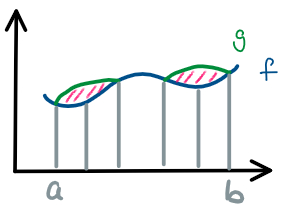
\includegraphics[scale=0.5]{Skizzen/plot_integral_zwei_fkt}
		\end{center}
		\caption{Flächeninhalt zweier Funktionen}
		\label{plot_flaeche_zweier_fkt}
	\end{figure}
	
	\item für $c \in [a,b]$ soll gelten (Abbildung~\ref{fig_integral_aufteilen})
	\begin{align*}
		\int_a^b f \dd{x} = \int_a^c f \dd{x} + \int_c^b f\dd{x}
	\end{align*}
	Vorgehen: Man unterteile $[a,b]$ in \enquote{viele} Teilintervalle, auf denen 
	$f$ nahezu konstant ist.
	\begin{figure}[ht]
\centering
	\begin{tikzpicture}
		\draw[very thin, gray, step = 0.5] (-0.9,-0.9) grid (4.9,2.9);
		\draw[->,thick, black](-1,0) -- (5,0) node[right]{x};
		\draw[->,thick, black](0,-1) -- (0,3) node[above]{y};
		\draw[blue,domain = 0.0:3.14, samples=1000]   
			plot (\x,{(\x * \x)*sin(\x r)*0.5+0.5});
       	\draw[green,thick](0.0,0)--(0.0,2.5)node[right]{a};
       	\draw[red,thick](3.14,0) -- (3.14,2.5) node[above]{b};
       	\draw[orange,thick](1.5,0) -- (1.5, 1.62) node[above]{c};
	\end{tikzpicture}
	\caption{Integral aufteilen}
	\label{fig_integral_aufteilen}
\end{figure}
\end{itemize} 

\begin{Definition}{
	Sei $ I \subseteq \mathbb{R}$ ein Intervall. Eine \underline{Partition}\todo{das geht besser auch mit Stichwortverzeichnis. Baue ich später ein.} $P$ 
	(Abbildung~\ref{fig_int_partition}) von 
	$[a,b]$ ist eine endliche Menge von Punkten $a = x_0 \leq x_1 \leq \hdots
	\leq x_n = b$.\\
	Wir schreiben $\Delta x_i = x_i - x_{i-1}$
	\begin{figure}[ht]
       \tikzsetnextfilename{plot_integral_partition}
       \begin{center}
              \begin{tikzpicture}
       		\draw[dotted, very thin, gray, step = 0.5] (-0.9,-0.9) grid (4.9,2.9);
       		\draw[->,thick, black](-1,0) -- (5,0) node[right]{x};
       		\draw[->,thick, black](0,-1) -- (0,3) node[above]{y};
       		\draw[blue,domain = 0.0:3.14, samples=1000]   
       			plot (\x,{(\x * \x)*sin(\x r)*0.5+0.5});
              	\draw[green,thick](0.0,0)--(0.0,2.5)node[right]{a};
              	\draw[red,thick](3.14,0) -- (3.14,2.5) node[above]{b};
              	\draw[black,thick](0.25,0) -- (0.25, 0.5)node[above]{$x_1$};
              	\draw[black,thick](0.5,0) -- (0.5, 0.55);
              	\draw[black,thick](1,0) -- (1, 0.92);
              	\draw[black,thick](1.25,0) -- (1.25, 1.24);
              	\draw[black,thick](1.5,0) -- (1.5, 1.62);
              	\draw[black, thick](2,0) -- (2, 2.31) node[above]{$x_i$};
              	\draw[black,thick](2.5,0) -- (2.5, 2.37);
              	\node at (4,1.5){$\int_a^b f$};
       	\end{tikzpicture}
       \end{center}
	\caption{Partition}
	\label{fig_int_partition}
\end{figure}
}\end{Definition}

\begin{Definition}{ \label{def_riemann-integrierbar}
	Sei $f : [a,b] \rightarrow \mathbb{R}$ beschränkt und $P = \{x_0, \hdots, x_n\}$ 
	eine Partition von $[a,b]$.\\
	Wir schreiben: 
	\begin{align*}
		M_i(P) := \sup_{x \in [x_{i-1}, x_i]} f(x) \\
		m_i(p) := \inf_{x \in [x_{i-1}, x_i]} f(x)
	\end{align*}
	Weiter definieren wir: 
	\begin{align*}
		S(P,f) := & \sum_{i=1}^n M_i \cdot \Delta x_i \\
		s(P,f) := & \sum_{i=1}^n m_i \cdot \Delta x_i
	\end{align*}
	Wir setzen:
	\begin{align*}
		\overline{\int_a^b} f \dd{x} = \inf S(P,f) \\
		\underline{\int_a^b} f \dd{x} = \sup s(P,f)
	\end{align*}
	wobei Infimum und Supremum über alle Partitionen von $[a,b]$ genommen werden. 
	Wir nennen 
	\begin{align*}
		& \overline{\int_a^b} f \dd{x} \text{ das \underline{obere} und} \\
		& \underline{\int_a^b} f \dd{x} \text{ das \underline{untere}}
	\end{align*}
	\underline{Riemannintegral} von $f$ über $[a,b]$ \\
	Gilt 
	\begin{align*}
		\int_a^{\overline{b}} f \dd{x} = \int_{\underline{a}}^b f \dd{x}
	\end{align*}
	sagen wir $f$ ist \underline{Riemann-integrierbar} (\underline{integrierbar}) 
	und nennen 
	\begin{align*}
		\int_a^b f(x) \dd{x} := \underline{\int_a^b} f \dd{x} = 
		\overline{\int_a^b} f \dd{x}
	\end{align*}
	das \underline{Riemannintegral} von $f$ über $[a,b]$.\\
	Die Menge der Riemanintegrierbaren Funktionen auf $[a,b]$ bezeichnen wir 
	mit $\mathcal{R}$ beziehungsweise $\mathcal{R}_{[a,b]}$.\\
	\begin{figure}[ht]
\centering
	\begin{tikzpicture}
		\draw[very thin, gray, step = 0.5] (-1.9,-0.9) grid (1.9,3.4);
		\fill[yellow](-1.5,0) rectangle (-0.75,3.25);
		\fill[orange](-0.75,0) rectangle (0,1.56);
		\fill[yellow](0,0) rectangle (0.75, 1.56);
		\fill[orange](0.75,0) rectangle (1.5,3.25);
		\draw[->,thick, black](-2,0) -- (2,0) node[right]{x};
		\draw[->,thick, black](0,-1) -- (0,3.5) node[above]{y};
		\draw[blue, domain = -1.5 :1.5]  
			plot(\x, \x * \x + 1);
	\end{tikzpicture}
	\caption{oberes Riemann-Integral}
	\label{fig_int_riemann}
\end{figure}
	\textbf{Bemerkungen}
	\begin{itemize}
		\item Da $f$ beschränkt ist, gibt es $m \leq M$ in $\mathbb{R}$ mit:
		\begin{align*}
			m \leq f(x) \leq M \text{ }(x \in [a,b])
		\end{align*}
		Damit gilt für jede jede Partition $P$: 
		\begin{align*}
			m \cdot (b-a) \leq s(P,f) \leq S(P,f) \leq M \cdot (b-a)
		\end{align*}
		Ergo: $\overline{\int_a^b} f \dd{x} , \underline{\int_a^b} f \dd{x}$ 
		sind wohldefiniert.
		\item im gesamten Kapitel~\ref{kap_riemann_integral}
		werden wir Funktionen stets als 
		beschränkt annehmen
	\end{itemize}
	
}\end{Definition}

\begin{Definition}{
	Seien $P_1, P_2$ zwei Partitionen eines Intervalls. Dann heißt $P_1$ 
	\underline{Verfeinerung} von $P_2$, wenn gilt: $P_2 \subseteq P_1$ \\
	Weiterhin nennen wir $P_1 \cup P_2$ die \underline{gemeinsame} Verfeinerung 
	von $P_1$ und $P_2$
}\end{Definition}

\begin{Satz}{\label{kap09_satz16}
	Ist $P'$ eine Verfeinerung der Partition $P$ von $[a,b]$, dann gilt:
	\begin{align*}
		S (P,f) \geq & S (P',f) \\
		s(P,f) \leq & s(P',f)
	\end{align*}
	(wobei $f$ wie in Definition~\ref{def_riemann-integrierbar}
	sei) \\
	\textbf{Beweis:} Wir zeigen nur die obere Ungleichung, die andere folgt analog. 
	Wir nehmen zunächst an, dass $P'$ sich von $P$ in nur einem Element $x'$ 
	unterscheidet. Das heißt: $P' = P \cup \{x'\}$ \\
	Dann gibt es ein $i \in \mathbb{N}$ mit $x' \in [x_{i-1}, x_i]$ \newline
	(wobei $P = \{x_0, x_1, \hdots, x_{i-1}, x_i, \hdots, x_n \}$ sei).\\
	Wir definieren:
	\begin{align*}
		W_1 := & \sup_{[x_{i-1}, x']} f(x) \\
		W_2 := & sup_{[x', x_i]} f(x)
	\end{align*}
	Dann gilt: 
	\begin{align*}
		S(P,f) - S(P',f) = &M_i \Delta x_i - W_1\cdot (x' - x_{i-1}) - 
		W_2\cdot (x_i - x') \\
		= & (M_i -W_1) \cdot (x' - x_{i-1}) 
		+ (M_i - W_2)\cdot(x_i - x') \geq 0
	\end{align*}
	 Enthält von $P'$ $k$ Punkte, die nicht in $P$ enthalten sind, so führen wir 
	 obiges Verfahren insgesamt $k$-mal durch. 
	
}\end{Satz}

\begin{Satz}{\label{kap09_satz17}
	Sei $f: [a,b] \rightarrow \mathbb{R}$ beschränkt. Dann gilt:
	\begin{align*}
		\obint a b f \geq \unint{a}{b} f
	\end{align*}
	\textbf{Beweis:} Seien $P_1, P_2$ zwei Partitionierungen von $[a,b]$ und 
	$P'$ die gemeinsame Verfeinerung. Dann gilt:
	\begin{align*}
		s(P_1,f) \leq s(P',f) \leq S(P',f) \leq S(P_2, f) 
	\end{align*}
	Mit anderen Worten:
	\begin{align*}
		s(P_1, f) \leq S(P_2, f)
	\end{align*}
	für alle Partitionierungen $P_1, P_2$. \\
	Sprich: $S(P_2,f)$ ist stets obere Schranke von $s(P,f)$ für alle Partitionen 
	$P$ von $[a,b]$. Ergo:
	\begin{align*}
		\sup s(P,f) \leq S (P_2, f)
	\end{align*}
	Damit ist also $\sup s(P,f)$ untere Schranke von $S(P,f)$ ($P$ beliebige 
	Partition). \\
	Ergo: $\sup s(P,f) \leq \inf S (P,f)$  \\
	Wir haben also gezeigt:
	\begin{align*}
		\int_{\underline{a}}^b f \dd{x} = \sup s(P,f) \leq 
		\inf S(P,f) = \inf \obint ab f 
	\end{align*}
}\end{Satz}
%!TEX root = ../gesamt.tex

\begin{Satz}{\label{kap_10_satz18}
	Sei $f: [a,b] \rightarrow \mathbb{R}$ beschränkt. Dann ist 
	$f \in \mathcal{R}_{[a,b]}$ genau dann, wenn für jedes $\epsilon > 0$ eine 
	Partition $P_{\epsilon}$ existiert mit:
	\begin{align*}
		S(P_2,f) - s(P_2,f) < \epsilon
	\end{align*}
}\end{Satz}

\begin{proof}
	 Per Definition gilt 
	\begin{align*}
		s(P_{\epsilon},f) \leq \underline{\int_{a}^b} f \dd{x}
		\overset{Satz~\ref{kap09_satz17}}{\le} \overline{\int_a^b} f \dd{x} 
		\leq S(P_{\epsilon},f) 		
	\end{align*}

	Damit erhalten wir:
	\begin{align*}
		\overline{\int_a^b} f \dd{x} - 
		\underline{\int_{a}^b} f \dd{x} \leq S(P_{\epsilon},f) 
		- s(P_{\epsilon},f) < \epsilon
	\end{align*}
	Das heißt, da $\epsilon$ beliebig, dass:
	\begin{align*}
		\underline{\int_{a}^b} \dd{x} = \overline{\int_a^b} f \dd{x}
	\end{align*}
	Ergo: $f \in \mathcal{R}_{[a,b]}$ \\
	Per Definition gibt es für alle $\epsilon > 0$ ein $P_{\epsilon}'$ mit:
	\begin{align}
		\label{gleichung_1_1505}
		\underline{\int_{a}^b} f \dd{x} - s(P_{\epsilon}',f) < \frac{\epsilon}{2} 
	\end{align}
	Analog existiert ein $P_{\epsilon}''$ mit 
	\begin{align}
		\label{gleichung_2_1505}
		S(P_{\epsilon}'',f) - \overline{\int_a^{b}} f \dd{x}) < \frac{\epsilon}{2}
	\end{align}
	Wir setzten $P_{\epsilon}$ gleich der gemeinsamen Vereinigung von 
	$P_{\epsilon}'$ und $P_{\epsilon}''$. Man beachte: Wegen Satz~\ref{kap09_satz16} 
	gelten Gleichung~\ref{gleichung_1_1505} und Gleichung~\ref{gleichung_2_1505},
	wenn wir $P_{\epsilon}'$, beziehungsweise $P_{\epsilon}''$, durch $P_{\epsilon}$
	ersetzen. Da $f \in \mathcal{R}_{[a,b]}$ gilt außerdem:
	\begin{align*}
		\underline{\int_{a}^b} f \dd{x} = \overline{\int_a^{b}} f\dd{x}
	\end{align*}	 
	Addition von Gleichung~\ref{gleichung_1_1505} und Gleichung~
	\ref{gleichung_2_1505} liefert:
	\begin{align*}
	S(P_{\epsilon},f) - s(P_{\epsilon},f) < \epsilon
	\end{align*}
\end{proof}

\begin{Satz}{\label{kap10_satz19}
	Sei $f:[a,b] \rightarrow \mathbb{R}$ beschränkt und $P_{\epsilon} = 
	\{x_0, \hdots, x_n\}$ eine Partition von $[a,b]$ mit $S(P_{\epsilon},f) -
	s(P_{\epsilon},f) < \epsilon$ für ein $\epsilon > 0$.
	\begin{enumerate}
		\item Ist $P$ eine Verfeinerung von $P_{\epsilon}$, so gilt 
		$S(P,f) - s(P,f) < \epsilon$
		\item Sind $s_i, t_i$ beliebige Punkte in $[x_{i-1},x_i]$, so gilt:
		\begin{align*}
			\sum_{i=1}^n \left\vert f(s_i) - f(t_i) \right\vert \cdot 
			\Delta x_i < \epsilon
		\end{align*}
		\item Ist $f \in \mathcal{R}_{[a,b]}$ und $t_i \in [x_{i-1},x_i]$, so 
		gilt 
		\begin{align*}
			\left\vert \sum_{i=1}^n f(t_i) \cdot \Delta x_i - \int_a^b f \dd{x} 
			\right\vert < \epsilon
		\end{align*}
	\end{enumerate}	
}\end{Satz}

\begin{proof}
	\begin{enumerate}
		\item[ ]
		\item Das folgt aus Satz~\ref{kap09_satz16}
		\item
		 \begin{align*}
			\sum_{i = 1}^n \left\vert f(s_i) - f(t_i) \right\vert	\cdot 
			\Delta x_i \leq \sum_{i=1}^n (M_i-m_i)\cdot \Delta x_i
			= S(P_{\epsilon},f) - s(P_{\epsilon},f) < \epsilon
		 \end{align*}
		 \item Da $t_i \in [x_{i-1},x_i]$, gilt $m_i \leq f(t_i) \leq M_i$ \\
		 	Damit folgt die Aussage aus
			 \begin{align*}
			 	s(P_{\epsilon},f ) \leq  
			 	\sum_{i = 1}^n m_i \cdot \Delta x_i \leq \sum_{i=1}^n f(t_i) \cdot \Delta 
			 	x_i \leq \sum_{i=1}^n M_i \cdot \Delta x_i = S(P_{\epsilon},f)
			 \end{align*}
			 und $s(P_{\epsilon},f) \leq \int_a^b f \dd{x} \leq S(P_{\epsilon},f)$
	\end{enumerate}
\end{proof}
	Wir wollen im Folgenden wichtige Vertreter Riemann-integrierbarer 
	Funktionen kennenlernen.

\begin{Satz}{\label{kap10_satz20}
	Ist $f: [a,b] \rightarrow \mathbb{R}$ stetig, so ist 
	$ f \in \mathcal{R}_{[a,b]}$.
}\end{Satz}

\begin{proof}
	Da stetige Funktionen auf abgeschlossenen Intervallen 
	beschränkt sind, ist $f$ offensichtlich beschränkt. Weiterhin ist $f$ als stetige 
	Funktion auf dem abgeschlossenen Intervall $[a,b]$ gleichmäßig stetig. \\
	Sei $\epsilon > 0 $ gegeben. Wegen der gleichmäßigen Stetigkeit von $f$ 
	existiert ein $\delta > 0$, so dass folgende Implikation gilt:
	\begin{align*}
		\vert x - y \vert < \delta \Rightarrow \vert f(x) -f(y) \vert < \epsilon
	\end{align*}
	Wir wählen eine Partition $P_{\epsilon} = \{ x_0, \hdots, x_n \}$, so dass 
	$\Delta x_i < \delta$. Dann gilt:
	\begin{align*}
		M_i - m_i < & \epsilon \text{ und daher} \\
		S(P_{\epsilon},f) - s(P_{\epsilon},f) = & \sum_{i = 1}^n (M_i -m_i)\Delta x_i 
		\leq \epsilon \cdot \sum_{i = 1}^n \Delta x_i = \epsilon \cdot (b-a)
	\end{align*}
	Da $\epsilon > 0$ beliebig, folgt die Aussage mit Satz~\ref{kap_10_satz18}.
\end{proof}

\begin{Satz}{
		Ist $f: [a,b] \rightarrow \mathbb{R}$ monoton, so ist 
		$f \in \mathcal{R}_{[a,b]}$ 
}\end{Satz}

\begin{proof}
	 Da $f$ monoton ist, gilt für alle $x \in [a,b]: f(a) \leq f(x) 
	\leq f(b)$. \\
	Das heißt $f$ ist beschränkt. Zu $n \in \mathbb{N}$ wählen wir eine 
	Partition \linebreak $P_n = \{x_0, \hdots, x_k\}$ mit $\Delta x_i < \frac{1}{n}$.
	\begin{figure}
	\begin{center}
	\tikzsetnextfilename{monotone_fkt_riemann_intbar}
		\begin{tikzpicture}
			\draw[very thin, gray, step = 0.5] (0,-0.9) grid (3.4,2.4);
			
			\draw[->, thick, black](0,-0.5) -- (3.5,-0.5) node[right]{x};
			\draw[->, thick, black](0.5, -1) -- (0.5, 2.5) node[above]{y};
			\draw[blue, domain = 1 :1.5, samples = 1000]  
				plot(\x, {\x * \x * sin(\x r) - \x });
			
			\draw[blue, domain = 2 :3, samples = 1000]  
				plot(\x, {\x * \x * sin(0.5*\x r) - \x*\x + 2});	
			
			\draw[fill=black](1,-0.16)circle(1pt);
			\draw[fill = black](1.3,0.33) circle(1pt);
			\draw[fill = black] (1.5, 0.74) circle(1pt);
			\draw[thick, black](1,-0.5) -- (1, -0.16);
			\draw[thick, black](1.3,-0.5) --(1.3, 0.33);
			\draw[thick, black](1.5,-0.5) --(1.5, 0.74);
			
			\draw[fill = black](2.1,1.42) circle (1pt);
			\draw[fill = black](2.9,1.94) circle(1pt);
			\draw[thick, black](2.1, -0.5) -- (2.1, 1.42);
			\draw[thick, black](2.9, -0.5) -- (2.9, 1.94);
		
		\end{tikzpicture}
	\end{center}
	\caption{Monotone Funktion}
	\label{fig:Monotone_Funktion_Riemannint}
\end{figure}
	Dann gilt:
	\begin{align*}
		S(P_n, f) - s(P_n,f) = & \sum_{i=1}^n (M_i - m_i)\Delta x_i
	\end{align*}
	Ohne Einschränkung sei $f$ monoton wachsend (der andere Fall läuft analog).
	Dann gilt:
	\begin{align*}
		M_i = & f(x_i) \text{ und} \\
		m_i = & f(x_{i-1})
	\end{align*} und daher:
	\begin{align*}
		S(P_n, f) - s(P_n,f) = & \sum_{i=1}^n (f(x_i) -f(x_{i-1}))\cdot \Delta x_i 
		\\ \leq & \frac{1}{	n}\sum_{i=1}^n f(x_i) -f(x_{i-1}) = 
		\frac{1}{n} (f(b) -f(a)) 
	\end{align*}
	Sei $\epsilon > 0$ gegeben. Wähle $n_{\epsilon}$ so dass gilt:
	\begin{align*}
		\frac{1}{n_{\epsilon}}(f(b) -f(a)) < \epsilon
	\end{align*}
	Dann gilt mit $P_{\epsilon} := P_{n_{\epsilon}}$ die Aussage nach Satz~\ref{kap_10_satz18}
\end{proof}

\begin{Satz}{\label{kap10_satz21}
	Sei $f: [a,b] \rightarrow \mathbb{R}$ beschränkt mit endlich vielen 
	Unstetigkeitsstellen %(Abbildung~\ref{plot_fkt_unstetigketsstellen}. 
	Dann gilt $f \in \mathcal{R}_{[a,b]}$.\\
	\begin{figure}[ht]
		\begin{center}
			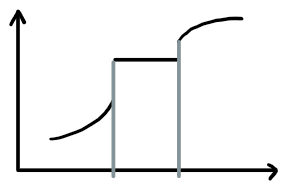
\includegraphics[scale=0.5]{Skizzen/plot_fkt_unstetigkeitsstellen}
		\end{center}
		\caption{Funktion mit endlich vielen Unstetigkeitsstellen}
		\label{plot_fkt_unstetigketsstellen}
	\end{figure}
}\end{Satz}

\begin{proof}
	 Sei $\epsilon > 0$ gegeben und $E = \{P_1, \hdots, P_n\}$
	die Menge der Unstetigkeitsstellen von $f$. Wir nehmen der Einfachheit halber 
	an, dass $\{a,b\} \cap E = \emptyset$ (der andere Fall läuft analog).
	Sei
	\begin{align*}
		 M:= \sup_{x \in [a,b]} \vert f(x) \vert
	\end{align*}
	 Wir wählen $u_j, v_j \in [a,b]$, 
	$j = (1, \hdots, n)$, so dass
	\begin{align*}
		P_s \in [u_j, v_j] \text{ und} \\
		2M (u_j - v_j) < \frac{\epsilon}{2n}
	\end{align*}		
	 Sei 
	 \begin{align*}
		I_1^{\epsilon} = & [a, u_1], \\
		 I_l^{\epsilon} = & [v_{l-1}, u_l] \text{ }  (l = 2, \hdots, n) \\
		 I_n^{\epsilon} = & [v_n, b]
	 \end{align*}
	Per Voraussetzung ist $f_{\vert I_j^{\epsilon}} (j = 1,\hdots, n+1)$ stetig. \\
	Daher existiert nach Satz~\ref{kap10_satz20}
	eine Partition $P_j^{\epsilon}$, so dass:
	\begin{align*}
		S(P_j^{\epsilon}, f_{I_j{\epsilon}}) - s(P_j^{\epsilon}, f_{I_j^{\epsilon}}) 
		 < \frac{\epsilon}{2(n+1)}
	\end{align*}
	Wir setzen $P^{\epsilon} = \cup_{l = 1}^n P_l^{\epsilon}
	 \cup U_{l=1}^n\{u_l,v_l\}$.\\
	 Dann gilt:
	 \begin{align*}
	 	S(P^{\epsilon},f) - s(P^{\epsilon},f) 
	 	= & \sum_{l=1}^{n+1} S(P_l^{\epsilon},f_{|I_l^{\epsilon}}) - 
	 		s(P_l^{\epsilon},f_{|I_l^{\epsilon}})  \\
	 		& + \sum_{l = 1}^n \left( \sup_{x \in [u_l, v_l]} 
	 		f(x) - \inf_{x \in [u_l, v_l]} f(x) (v_l - u_l)\right) \\
	 		\leq & \sum_{l=1}^{n+1} \frac{\epsilon}{2(n+1)} + \sum_{l=1}^n
	 			2M \cdot(v_l-u_l) \leq \frac{\epsilon}{2} + \frac{\epsilon}{2} 
	 			= \epsilon
	 \end{align*}	 
\end{proof}

\begin{Definition}{
	Eine Funktion $f: [a,b] \rightarrow \mathbb{R}$ heißt \emph{Treppenfunktion}
	 (Abbildung~\ref{plot_treppenfkt}), 
	wenn es 
	eine Partition $Z = \{ y_0, \hdots, y_m \}$ von $[a,b]$ gibt und für alle 
	$i \in \{0, \hdots, m\}$ für $c_i \in \mathbb{R}$ gibt, so dass:
	\begin{align*}
		f(x) = c_i \text{ } ( x\in (y_{i-1},y_i))
	\end{align*}
	gilt.
	\begin{figure}
		\begin{center}
			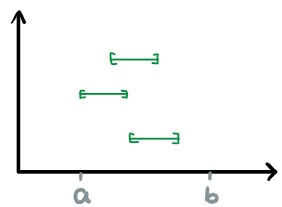
\includegraphics[scale=0.5]{Skizzen/plot_treppenfkt}
		\end{center}
		\caption{Treppenfunktion}
		\label{plot_treppenfkt}
	\end{figure}
	Nach Satz~\ref{kap10_satz21}
	ist jede Treppenfunktion Riemann-integrierbar. \\
	Zur Berechnung des Intervalls bedienen wir uns der Notation von Satz 10 
	\todo{falsche Referenz -> hardgecodet; sollte Satz 3.7 sein}
	%\ref{kap10_satz21}
	und verwenden Satz~\ref{kap10_satz19}c.\\
	Zur Vereinfachung nehmen wir wieder an, dass $f$ in $a$ und $b$ stetig ist. 
	Das heißt die Menge der Unstetigkeitsstellen ist gegeben durch 
	$E = \{y_1, \hdots, y_{m-1}\}$. \\
	Für $x \in I_l^{\epsilon}$ gilt dann $f(x) = c_l$ für alle $ l = 1, \hdots, m$.
	Dann gilt nach Satz~\ref{kap10_satz19}c:
	\begin{align*}
		\left\vert \int_a^b f \dd{x} - \sum_{i=1}^{m+1} c_i \cdot \vert 
		I_l^{\epsilon}\vert + \sum_{i =1}^{m-1} f(y_i)\cdot (v_i -u_i) \right\vert
		< \epsilon
	\end{align*}
	Für $ \lim\limits_{\epsilon \rightarrow 0}{}$ gilt:
	$$\begin{cases} 
		|I_1^\epsilon| \rightarrow y_{1}-a & \\
		\vert I_l^\epsilon \vert \rightarrow y_l - y_{l-1} & ( l = 2,...,m) \\
		\vert I_{m+1}^{\epsilon} \vert \rightarrow b - y_m &
	\end{cases}$$
	Das heißt
	\begin{align}
		\label{gleichung_3_1705}
		\sum_{i=1}^{m+1}c_i \abs{I^{\epsilon}_l} \rightarrow c_1(y_1 -a) + 
		\sum_{i=2}^m c_i \cdot (y_i -y_{i-1}) + c_m(b-y_m)
	\end{align}
	Außerdem gilt $v_i-u_j \overset{\epsilon \rightarrow 0}{\rightarrow} 0$
	gilt $\int_a^b f\dd{x} = Gleichung~\ref{gleichung_3_1705}$
	
}\end{Definition}

\begin{Korollar}{
	Ist $f:[a,b] \rightarrow \mathbb{R}$ stetig, beziehungsweise monoton, beziehungsweise 
	besitzt $f$ höchstens endlich viele Unstetigkeitsstellen und ist beschränkt, so ist 
	$f \in \mathcal{R}_{[a,b]}$.
}\end{Korollar}

\begin{Bemerkung}{
	Mit Hilfe des Lebesguesches Integrabilitätskriterium kann man 
	sogar zeigen, dass beschränkte Funktionen mit abzählbar vielen Unstetigkeitsstellen 
	Riemann-integrierbar sind.
}\end{Bemerkung}

\begin{Beispiel}{
	\begin{align*}
		\int_0^a x \dd{x}
	\end{align*}
	Da $id :[0,a] \rightarrow \mathbb{R}$ stetig ist, existiert das Integral. \\
	Sei $P_n =\{ 0, \frac{a}{n}, \frac{2a}{n}, \hdots, \frac{(n-1)a}{n}, a\}$ 
	eine Partition von $[a,b]$. \\
	Es gilt: 
	\begin{align*}
		S(P_n, x) = & \sum_{i =1} ^n \frac{a_i}{n} \cdot \frac{a}{n} \\
		= & \frac{a^2}{n^2} \sum_{i = 1}^n i \\
		= & \frac{a^2}{n^2} \frac{n(n+1)}{2} \\ 
		= & \frac{a^2}{2} \cdot \left( 1 + \frac{1}{n} \right)
	\end{align*}
	\begin{align*}
		s(P_n, x) = & \sum_{i = 0}^n \frac{a_i}{n} \cdot \frac{a}{n}  \\
		= & \frac{a^2}{n^2} \cdot \frac{(n-1)n}{2} \\
		= & \frac{a^2}{2}\left( 1 - \frac{1}{n} \right)
	\end{align*}
	Da $id$ integrierbar ist, gilt:
	\begin{align*}
		\int_0^a x \dd{x} \in \left[ s(P_n,x), S(P_n, x)\right] = 
		\left[\frac{a^2}{2}- \frac{1}{n}, \frac{a^2}{2}+\frac{1}{n}\right]
		n \in \mathbb{N}
	\end{align*}
	Das heißt:
	\begin{align*}
		\int_0^a x \dd{x} \cap_{n \in \mathbb{N}} \left[\frac{a^2}{2}- \frac{1}{n}, 
		\frac{a^2}{2}+\frac{1}{n}\right]
	\end{align*}
	Also: $\int_0^a x \dd{x} = \frac{a^2}{2}$
}\end{Beispiel}

\begin{Beispiel}{
	Sei $D:[0,1] \rightarrow \mathbb{R}$ die \emph{Dirichlet-Funktion}, d.h
	\begin{align*}
		D(x) = \begin{cases}
			1 & \textit{falls } x \in \mathbb{Q} \\
			0 & sonst
		\end{cases}
	\end{align*}
	Daher gilt für jede Partition $P = \{x_0, \hdots, x_n\}$, dass 
	\begin{align*}
		M_i = & \sup_{x \in [x_{i-1}-x_i]} f(x) = 1 \text{ und}\\
		m_i = & \inf_{x \in [x_{i-1}-x_i]} f(x) = 0
	\end{align*}
	Damit gilt:
	\begin{align*}
		S(P,f) - s(P,f) = \sum_{i = 1}^n (M_i - m_i) \cdot \Delta x_i 
		= \sum_{i = 1}^n \Delta x_i = 1
	\end{align*}
	Ergo: $D$ ist nicht Riemann-integrierbar
}\end{Beispiel}

\begin{Satz}{\label{vl_11_satz23}
	Sei $f \in \mathcal{R}_{[a,b]}$ und $m \leq f(x) \leq M$ $ (x \in [a,b])$.
	Sei ferner  \linebreak $\Phi : [m, M] \rightarrow \mathbb{R}$ stetig. 
	Dann ist $\Phi \circ f \in \mathcal{R}_{[a,b]}$ \\
	\textbf{Beweis:} Sei $\epsilon > 0$ gegeben. Da $\Phi$ auf dem abgeschlossenen Intervall 
	$[m,M]$ stetig ist, existiert ein $\delta > 0$ 
	(Ohne Eisnchränkung sei $\delta < \epsilon$) mit :
	\begin{align*}
		\vert s - t\vert < \delta \Rightarrow \vert f(x) - f(t) \vert < \epsilon
	\end{align*}
	Da $f$ integrierbar ist, gibt es eine Partition $P = \{x_0, \hdots, x_n\}$
	mit 
	\begin{align*}
		S(P,f) - s(P,f) < \delta^2
	\end{align*}		
	Wie üblich bezeichnen wir 
	\begin{align*}
		M_i = & \sup_{x \in [x_{i-1}-x_i]} f(x) \text{ und } \\
		m_i = & \inf_{x \in [x_{i-1}-x_i]} f(x) \text{ und weiterhin} \\
		M_i^+ = & \sup_{x \in [x_{i-1}-x_i]} \Phi \circ f \text{ sowie } \\
		m_i^* = & \inf_{x \in [x_{i-1}-x_i]} \Phi \circ f(x)
	\end{align*}		
	Seien
	\begin{align*}
		A = & \{i = 1, \hdots, n \vert M_i -m < \delta \} \\
		B = & \{ i = 1, \hdots, n\} \setminus A
	\end{align*}
	Aufgrund der Wahl von $\delta$ gilt für alle $ i \in A: M_I^+ - m_i^* < \epsilon$
	Weiter gilt: 
	\begin{align*}
		\delta \cdot \sum_{i \in B} \Delta x_i = \sum_{i \in B} \delta \cdot \Delta x_i 
		\leq  \sum_{i \in B} (M_i - m_i) \Delta x_i \leq \delta^2
	\end{align*}
	Ergo: $\sum_{i \in B} \Delta x_i \leq \delta$. \\
	Damit gilt:
	\begin{align*}
		S(P, \Phi \circ f) - s(P, \Phi \circ f) = 
		& \sum_{i = 1}^n (M_i^+ - m_i^*) \cdot\Delta x_i  \\
		= & \sum_{i \in A} (M_i^+ - m_i^* ) \cdot \Delta x_i + 
			\sum_{i \in B} (M_i^+ -m_i) \Delta x_i \\
		\leq & \epsilon \sum_{i \in A}\Delta x_i + 2 \sup_{x \in [m,M]} \abs{
			\Phi \circ f} \cdot \sum_{i \in B} \Delta x_i \\
		\leq & \epsilon \left(|b-a| + 2\sup_{x \in [m,M]} \abs{\Phi \circ f(x)}\right)
	\end{align*}
	Da $\epsilon > 0$ beliebig, folgt die Behauptung mit~\ref{kap_10_satz18}.
}\end{Satz}

\begin{Satz}{\label{vl_11_satz24}%12
	Seien $f_1, f_2,f \in \mathcal{R}_{[a,b]}$ Dann gilt:
	\begin{enumerate}
		\item 
		\begin{align*}
			\int_a^b f_1 +f_2 \dd{x} = \int_a^b f_1\dd{x} + \int_a^b f_2 \dd{x}
		\end{align*}
		und für $c \in \mathbb{R}$ gilt:
		\begin{align*}
			\int_a^b c f\dd{x} = c \int_a^b f\dd{x}
		\end{align*}
		\item Insbesondere gilt also 
		\begin{align*}
			f_1 + f_2 \in \mathcal{R}_{[a,b]} \text{und} \\
			c f \in \mathcal{R}_{[a,b]}
		\end{align*}
		\item Gilt $f_1(x) \leq f_2(x) \text{ } ( x \in [a,b])$ so folgt
		\begin{align*}			
			\int_a^b f_1 \dd{x} \leq \int_a^b f_2 \dd{x}
		\end{align*}
		\item Ist $c \in (a,b)$, und $f \in \mathcal{R}_{[a,b]}$ so gilt
		\begin{align*}
			\int_a^b f\dd{x} = \int_a^c f\dd{x} + \int_c^b f \dd{x}
		\end{align*}
		\item Gilt $M \geq f(x)$ $(x \in [a,b])$ so gilt 
		\begin{align*}
			M \cdot (b-a) \geq \int_a^b f \dd{x}
		\end{align*}
	\end{enumerate}
	\textbf{Beweis:}
	\begin{enumerate}
		\item Da $f_i \in \mathcal{R}_{[a,b]} (i = 1, 2)$ gibt es Partitionen 
		$P_i$ von $[a,b]$ mit 
		\begin{align*}
			S(P_i,f) - s(P_i,f) \leq \epsilon \text{ für ein festes } \epsilon > 0
		\end{align*}
		Dann gilt für die gemeinsame Verfeinerung $P = P_1 \cup P_2 = \{x_0, \hdots
		x_n\}$ nach Satz~\ref{kap09_satz16}
		, dass 
		\begin{align*}
			S(P,f_i) - s(P, f_i) \leq \epsilon \text{ }(i = 1,2)
		\end{align*}		 
		\item Es gilt 
		\begin{align*}
			\sup_{x \in [x_{i-1}-x_i]} f_1(x) +f_2(x) \leq & 
			\sup_{x \in [x_{i-1}-x_i]} f_1(x) + \sup_{x \in [x_{i-1}-x_i]} f_2(x)
		\end{align*}				
		Analog gilt: 
		\begin{align*}
			\inf_{x \in [x_{i-1}-x_i]} f_1(x) + f_2(x) \geq & 
			\inf_{x \in [x_{i-1}-x_i]} f_1(x) + \inf_{x \in [x_{i-1}-x_i]} f_2(x)
		\end{align*}				
		Damit folgt:
		\begin{align*}
			s(P,f_1) + s(P,f_2) \leq s(P,f_1 +f_2) \leq S(P,f_1 + f_2) 
			\leq S(P,f_1) + S(P,f_2)
		\end{align*}
		Also gilt:
		\begin{align*}
			S(P, f_1 + f_2) - s(P, f_1 +f_2) & \\
			\leq &  S(P, f_1) - s(P,f_1) + S(P,f_2) 
			-s(P,f_2) \leq 2 \epsilon
		\end{align*}
		Da $\epsilon >0 $ beliebig gewählt war, gilt $f_1 + f_2 \in 
		\mathcal{R}_{[a,b]}$ nach Satz~\ref{kap_10_satz18}. \\
		Weiter gilt: 
		\begin{align*}
			s(P, f_1 +f_2), S(P, f_1 + f_2) \in &
			[s(P,f_1) - s(P,f_2), S(P,f_1) + S(P,f_2)] \\
			\subseteq 
			& \left[ \int_a^b f_1 \dd{x} + \int_a^b f_2\dd{x} + 2\epsilon \right]
		\end{align*}
		Da $\epsilon > 0$ beliebig gewählt wurde, gilt:
		\begin{align*}
			\int_a^b f_1 + f_2 \dd{x}  = \int_a^b f_1\dd{x} + \int_a^b f_2 \dd{x}
		\end{align*}
		Die Aussage bezüglich  $c \cdot f$ zeigt man analog.
		\item Sei $f_2(x) \geq f_1(x)$ $(x \in [a,b])$. Dann gilt
		\begin{align*}		
			f_2(x) - f_1(x) \geq & 0 \text{ und daher} \\
			s(P, f_2 -f_1) \geq & 0
		\end{align*} 
		 für jede Partition $P$ von $[a,b]$ 
		Wegen 1 ist $f_2 -f_1 \in \mathcal{R}_{[a,b]}$ und es gilt:
		\begin{align*}
			\int_a^b f_2 \dd{x} = \int_a^b f_1 \dd{x} + \int_a^bf_2-f_1 \dd{x} 
			\geq \int_a^b f_1 \dd{x}
	\end{align*}		 
	\item Für 3. betrachtet man zu beliebiger Partition $P$ von $[a,b]$ die Partition \linebreak
	$P' = \{c\} \cup P$
	\item Folgt aus 2. mit $f_1 = f$ und $f_2 = M$ soweit 
	\begin{align*}
		\int_a^b M \dd{x} = M \cdot (b-a)
	\end{align*}		
	\end{enumerate}
}\end{Satz}

\begin{Bemerkung}{
	\begin{itemize}
	 	\item[ ]
		\item Eigenschaft 1 sagt, dass $\mathcal{R}_{[a,b]}$ ein bezüglich der Addition von 
		Funktionen und Multiplikation mit Skalaren ein Vektorraum ist
		\item Eigenschaft 1 sagt weiterhin, dass die Abbildung 
		\begin{align*}
			\int_a^b \dd{x} : \mathcal{R}_{[a,b]} \rightarrow  & \mathbb{R} \\
			f \mapsto & \int_a^b f\dd{x}
		\end{align*}
		ein lineares Funktionsglied\todo{Das Wort ist glaube ich falsch. Lineares Funktional könnte stimmen} ist
		\item Eigenschaft 2 sagt, dass dieses Funktional positiv ist
		(also nicht-negative Funktionen einen nicht negativen Wert zuordnet)
		\item Eigenschaft 4 impliziert eine gewisse stetigkeit
	\end{itemize}
}\end{Bemerkung}

\begin{Satz}{
	Für $f,g \in \mathcal{R}_{[a,b]}$ gilt:
	\begin{itemize}
		\item $f \cdot g \in \mathcal{R}_{[a,b]}$
		\item $\abs{f} \in \mathcal{R}_{[a,b]}$ und $\int_a^b \abs{f} \dd{x} 
		\geq \abs{\int_a^b f \dd{x}}$
	\end{itemize}
	\textbf{Beweis:}
	Sei $\Phi : \mathbb{R} \rightarrow  \mathbb{R}, t \mapsto t^2$. \\
	Dann ist
	$\Phi$ stetig und damit $\Phi \circ (f+g) $ bzw $\Phi \circ (f -g)$ 
	aufgrund von Satz~\ref{vl_11_satz24} und Satz~\ref{vl_11_satz23}
	Riemann-integrierbar über $[a,b]$.
	Beachte: 
	\begin{align*}
		f g = \frac{1}{4} ((f + g)^2 - (f-g)^2) \in \mathcal{R}_{[a,b]}
	\end{align*}
	\item Nach Satz~\ref{vl_11_satz23}
	gilt wieder $\abs{f} \in \mathcal{R}_{[a,b]}$. Sei nun $c \in \{-1, 1\}$ so 
	gewählt, dass 
	\begin{align*}
		c \int_a^b f \dd{x} \geq 0
	\end{align*}
	Offensichtlich gilt 
	\begin{align*}
		\abs{f(x)} = \abs{c f(x)} \geq c f(x) \quad (x \in [a,b])
	\end{align*}
	Damit gilt mit Satz~\ref{vl_11_satz24}
	\begin{align*}
		\abs{\int_a^b f\dd{x}} = c \int_a^b f\dd{x} = \int_a^b cf \dd{x} 
		\overset{Satz~\ref{vl_11_satz24}}{\le} \int_a^b \abs{f}\dd{x}
	\end{align*}
}\end{Satz}

\begin{Satz}[Mittelwertsatz der Integralrechnung]{
	Seien $f,g: [a,b] \rightarrow \mathbb{R}$ stetig und 
	$g(x) \geq 0$ $(x \in[a,b])$. \\
	(Abbildung~\ref{plot_MWS_int}) 
	\begin{figure}
	\begin{center}
		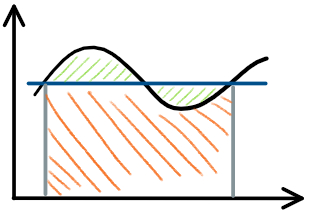
\includegraphics[scale=0.5]{Skizzen/mws_int}
	\end{center}
	\caption{Mittelwertsatz der Integralrechnung}
	\label{plot_MWS_int}
	\end{figure}		
	
	Dann existiert ein $\xi \in [a,b]$ mit 
	\begin{align*}
		\int_a^b f g \dd{x} = f(\xi) \int_a^b g\dd{x}
	\end{align*}
	\textbf{Bemerkung:}
	Für $g = 1$ gilt dann: 
	\begin{align*}
		\int_a^b f \dd{x} = f(\xi) \cdot (b-a)
	\end{align*}
	\textbf{Beweis:} Man setze: $h: [a,b] \rightarrow \mathbb{R},$ $y \mapsto f(y) 
	\cdot \int_a^b g \dd{x}$. $h$ ist stetig und es gilt:
	\begin{align*}
		\inf_{y \in [a,b]} h(y) = & \inf_{y \in [a,b]} \int_a^b f(y) g(x) \dd{x} \\
		\leq & \int_a^b \int_{y \in [a,b]} f(y) g(x) \dd{x} \\
		 \overset{Satz~\ref{vl_11_satz24}}{\le} & \int_a^bf(x)g(x) \dd{x} 
		\overset{Satz~\ref{vl_11_satz24}}{\le}
		\int_a^b \sup_{y \in [a,b]} f(y) g(x) \dd{x} = \sup_{y \in [a,b]} h(y)
	\end{align*}
	D.h wir haben eine stetige Funktion $h$ mit 
	\begin{align*}
		\int_a^b fg\dd{x} \in [\inf_{y \in [a,b]} h(y),  \sup_{y \in [a,b]} h(y)]
	\end{align*}
	\textbf{Bemerkung:} Wir haben bereits gesehen: Polynome sind beliebig oft
	 differenzierbar.
	
}\end{Satz}
%!TEX root = ../gesamt.tex

\cleardoublepage

\section{Differentiation und Integration}

\begin{Bemerkung}{
	Bisher hatten wir stets $\int_a^b f \dd{x}$ mit $ a \leq b$ betrachtet.
	Für $a \geq b$ setze man 
	\begin{align*}
		\int_a^b f \dd{x} := - \int_b^a f \dd{x}
	\end{align*}
}\end{Bemerkung}

\begin{Satz}{\label{vl_12_satz_01}
	Sei $f \in \mathcal{R}_{[a,b]}$. Für $ a \leq x \leq b$ setze man 
	\begin{align*}
		F(x) = \int_a^x f(t) \dd{t}
	\end{align*}
	Dann gilt
	\begin{enumerate}
		\item $F$ ist stetig auf $[a,b]$
		\item Ist $f$ stetig in $x_0 \in [a,b]$, so ist $F$ in $x_0$ differenzierbar 
		und es \linebreak gilt: $F'(x_0) = f(x_0)$
	\end{enumerate}
}\end{Satz}


\begin{proof}~
	\begin{enumerate}
		\item Da $f \in \mathcal{R}_{[a,b]}$, ist $f$ insbesondere beschränkt.
		Das heißt es existiert ein $M \in \mathbb{R}$ mit 
		\begin{align*}
			\forall x \in [a,b]:\abs{f(x)} \leq M
		\end{align*}
		Sei nun $\epsilon > 0$ gegeben. Setze $\delta := \frac{\epsilon}{M}$. 
		Für $x, y \in [a,b]$ mit $\abs{x-y} < \delta$ erhalten wir:
		\begin{align*}
			\abs{F(x) - F(y)} = & \abs{\int_a^x f \dd{t} - \int_a^y f \dd{t} }\\
			= &  \abs{ \left (\int_a^y f\dd{t} + \int_y^x f\dd{t} \right ) - \int_a^yf\dd{t}} \tag{Satz~\ref{vl_11_satz24}-4}\\
			= & \abs{\int_y^x f\dd{t}} \leq \int_y^x \abs{f} \dd{t} \tag{Satz~\ref{vl_11_satz_25}}\\
			\leq & M \cdot \int_y^x 1 \dd{t} = M (x-y) < \epsilon
		\end{align*}
		Da $\epsilon > 0$ beliebig gewählt war, folgt die Aussage
		\item Sei $h \in \mathbb{R}$, so dass $x_0 +h \in [a,b]$.
		Dann gibt es ein $\xi_h$ zwischen $x_0$ und $x_0+h$ mit:
		\begin{align*}
			\frac{F(x_0 + h) - F(x_0)}{h}
			= & \frac{ \int_a^{x_0+h}f(t)\dd{t}- \int_a^{x_0}f(t)\dd{t}}{h} \\
			= & \frac{h}{1} \int_{x_0}^{x_0+h} f(t)\dd{t} \\
			= & \frac{1}{h} f(\xi_h) \cdot \int_{x_0}^{x_0+h} \dd{t} \tag{Satz~\ref{satz:mws_integral}}\\
			= & \frac{1}{h} f(\xi_h) \cdot h
		\end{align*}
		 Damit gilt (wegen der Stetigkeit von $f$ in $x_0$):
		 \begin{align*}
		 \lim\limits_{h \rightarrow 0}{\frac{F(x_0+h)-F(x_0)}{h}} 
			= \lim\limits_{h \rightarrow 0} f(\xi_h) = f(x_0)
		 \end{align*}
	\end{enumerate}
\end{proof}


\begin{Satz}[Hauptsatz der Differential- und Integralrechnung]{\label{vl_12_satz_02}
	Ist $f \in \mathcal{R}_{[a,b]}$ und es gilt $F: [a,b] \rightarrow \mathbb{R}$
	differenzierbar mit $F' = f$. Dann gilt
	\begin{align*}
		\int_a^b f\dd{x} = F(b) - F(a) 
	\end{align*}
}\end{Satz}

\begin{Bemerkung}{
	~\begin{itemize}
		\item Eine Funktion $F$ mit $F'=f$ nennt man eine \emph{Stammfunktion} 
		von $f$
		\item Man schreibt gerne $F(x) \vert_a^b := F(b) -F(a)$
	\end{itemize}
}\end{Bemerkung}

\begin{proof}
	Sei $\epsilon >0 $ gegeben. Man wähle eine Partition $P = \{x_0, \hdots, x_n\}$ 
	mit 
	\begin{align*}
		S(P,f) - s(P,f) < & \epsilon
	\end{align*}
	Weiter existiert aufgrund des Mittelwertsatzes der \\Differential-Rechnung
	(Satz~\ref{vl_07_MWS}) 
	$\xi \in [x_{i-1}, x_i]$ mit 
	\begin{align*}
		F(x_i) - F(x_{i-1}) = &  f(\xi_i) \cdot \Delta x_i
	\end{align*}
	Nach Satz~\ref{kap10_satz19} gilt 
	\begin{align*}
		\epsilon > & \abs{ \int_a^b f \dd{x} - \sum_{i=1}^n f(\xi_i) \Delta x_i} \\
		= & \abs{ \int_a^b f \dd{x} - \sum_{i=1}^n F(x_i) -F(x_{i-1})} \\
		= & \abs{ \int_a^b f \dd{x} - (F(b) -F(a))}
	\end{align*}
	Da $\epsilon > 0$ beliebig gewählt war, folgt die Behauptung.	
\end{proof}

\begin{Bemerkung}{
	\begin{itemize}
	\item[ ]
		\item Sei $f \in \mathcal{R}_{[a,b]}$ Dann bezeichnet man die Funktion 
		\begin{align*}
			\int_a^{\circ} f\dd{x} :  [a,b]  & \rightarrow \mathbb{R} \\
			 t & \mapsto \int_a^b f\dd{x}
		\end{align*}
		\todo{ich bin mir hier nicht sicher ob das nicht t $\mapsto \int_a^x f \dd{t}$ sein müsste}
		als \emph{unbestimmtes Integral} von $f$.
		\item Satz~\ref{vl_12_satz_02}
		sagt also das jede Stammfunktion ein unbestimmtes Integral von $f$ ist 
	\end{itemize}
}\end{Bemerkung}

\begin{Proposition}{
	Sei $F: [a,b] \rightarrow \mathbb{R}$ eine Stammfunktion von $f \in \mathcal{R}
	_{[a,b]}$. Eine Funktion $G: [a,b] \rightarrow \mathbb{R}$ ist genau dann 
	Stammfunktion von $f$, wenn $F-G = konst.$
}\end{Proposition}

\begin{proof}
	 $\Leftarrow$ \\
	Sei $c \in \mathbb{R}$. Dann gilt für $F + c$ 
	\begin{align*}
		(F+ c)' = F' = f
	\end{align*}
	$\Rightarrow$ \\
	Das war eine Folgerung des Mittelwertsatzes der Differentialrechnung 
	(Satz~\ref{vl_07_MWS}).
\end{proof}

\begin{Bemerkung}{
	Oftmals wird ignoriert, dass sobald es eine Stammfunktion $F$ von $f$ gibt, es 
	automatisch unendlich viele gibt. So schreibt man beispielsweise 
	\begin{align*}
		\int f \dd{x} = F
	\end{align*} 
	oder spricht von \glqq der\grqq{} Stammfunktion. Die obige Gleichung ist
	 insofern problematisch, da die rechte Seite (und damit per Definition auch die 
	 linke Seite) nur bis auf eine Konstante bestimmt ist. Oftmals ist daher der 
	 etwas laxe Umgang mit den Begriffen unkritisch.
}\end{Bemerkung}

\begin{Satz}[Partielle Integration]{\label{vl_12_satz_03}
	Seien $F,G: [a,b] \rightarrow \mathbb{R}$ differenzierbar mit 
	\begin{align*}
		F' = f \text{ und } G' = g 
	\end{align*}
	wobei $f,g \in \mathcal{R}_{[a,b]}$. Dann gilt:
	\begin{align*}
		\int_a^b F \cdot g \dd{x} = FG\vert_a^b - \int_a^b f \cdot G \dd{x}
	\end{align*}
}\end{Satz}

\begin{proof}
	\begin{align}\label{vl_12_gl_1}
		\frac{\mathrm{d}}{dt}F(t)\cdot G(t) = & F(t)G(t) + F(t)G'(t) = 
		f(t)G(t) + F(t)g(t)
	\end{align}
	Da $f,g \in \riemann a b$ und $F,G$ differenzierbar (und daher auch in 
	$\riemann a b$), ist die rechte Seite in $\riemann a b$. \\
	Mit Satz~\ref{vl_12_satz_02} haben wir:
	\begin{align*}
		\int_a^b f(t) G(t) + F(t)g(t) \dd{t} = F(b)G(b) -F(a)G(a)
	\end{align*}
	Weiter aufgrund der Linearität des Integrals:
	\begin{align*}
		\int_a^bfG + Fg \dd{t} = \int_a^b fG\dd{t} + \int_a^b Fg\dd{t} \\
		\ref{vl_12_gl_1}-\int_a^b fG\dd{t}
	\end{align*}
	liefert die Behauptung.
\end{proof}

\begin{proof}
	\begin{align*}
		\left( FG|_a^x - \int_a^x f \cdot G \dd{t} \right)' = &
		\left(F(x) \cdot G(x) - F(a) \cdot G(a) - \int_a^x fG \dd{t} \right)' \\
		= & F'(x)G(x) + F(x)G'(x) - f(x)G(x)) \\
		= & f(x)G(x) + F(x)g(x) -f(x)G(x)
	\end{align*}
	Ergo: die rechte Seite ist eine Stammfunktion des Integranden der 
	linken Seite. Damit folgt die Aussage aus Satz~\ref{vl_12_satz_02}.
\end{proof}

\begin{Beispiel}{
	\begin{align*}
		& \int_a^b cos^2(x) \dd{x} & = &  \int_a^b cos(x) \cdot cos(x) \dd{x} \\
		& &  = & \left. cos(x) \cdot sin(x) \right\vert_a^b + 
			\int_a^b sin^2 \dd{x} \\
		& & = & \left. cos(x) \cdot sin(x) \right\vert_a^b + 
			\int_a^b 1 - cos^2(x) \dd{x} \\
		& & = & \left. cos(x) \cdot sin(x) \right\vert_a^b 
			+ \int_a^b 1 \dd{x} \\
		& & & - \int_a^b cos^2(x) \dd{x} 
			 \; \left\vert + \int_a^b cos^2(x) \dd{x} \right. \\
	 \Leftrightarrow 
	 & 2 \int_a^b cos^2(x) \dd{x} & = & \left. cos(x) \cdot sin(x) \right\vert_a^b 
	 	+ \left. x \right\vert_a^b  \left\vert \cdot \frac{1}{2} \right. \\
	 \Leftrightarrow
	& \int_a^b cos^2(x) \dd{x} & = & \frac{1}{2} \cdot 
		\left. \left( cos(x) \cdot sin(x) + x\right) \right\vert_a^b \\
	\text{Ergo: } & \int_a^b cos^2(x) \dd{x} & = & \frac{1}{2} (cos(x) sin(x) 
		\vert_a^b + (b-a))
	\end{align*}
	\begin{align*}
		\int_a^b \ln (x) \dd{x} \text{ wobei } 0 \not\in [a,b] \\
		\int 1 \cdot \ln (x) \dd{x} = & x \cdot \ln (x)\vert_a^b - 
		\int_a^b x \cdot \frac{1}{x} \dd{x} \\
		= & \left. x \cdot \ln (x) \right\vert_a^b - \int_a^b 1 \dd{x} \\
		= & \left. x \cdot \ln (x)\right\vert_a^b - \left. x\right\vert_a^b \\
		= & \left. x \cdot \ln (x)\right\vert_a^b - (b - a)
	\end{align*}
}\end{Beispiel}

\begin{Satz}{\label{vl_12_satz_04}
	Sei $f: [a,b] \rightarrow \mathbb{R}$ stetig und $\phi: [c,d] \rightarrow [a,b]$ 
	stetig differenzierbar. Dann gilt:
	\begin{align*}
		\int_a^b f(\phi(t))\cdot\phi'(t)\dd{t} = \int_{\phi(c)}^{\phi(d)} 
		f(x) \dd{x}
	\end{align*}	 
}\end{Satz}


\begin{proof}
	Sei $F : [a,b] \rightarrow \mathbb{R}$ eine Stammfunktion von $f$. Dann gilt für 
	$t \in [c,d]$:
	\begin{align*}
		\frac{\mathrm{d}}{\mathrm{dt}}F(\phi(t)) = &  F'(\phi(t)) \cdot \phi'(t) \\
		= & f(\phi(t))\cdot \phi'(t) \\
		\text{Ergo: } \int_{\phi(c)}^{\phi{d}} = & \int F(\phi(d))-F(\phi(c)) \\
		= & \int_a^b f(\phi(t)) \phi'(t) \dd{t}
	\end{align*}
\end{proof}

\begin{Bemerkung}{
	\begin{itemize}
		\item[ ]
		\item Die Substitutionsregel lässt sich wie folgt nachrechnen
		\begin{align*}
			\phi'(t)\mathrm{dt} = \frac{\mathrm{d\phi}}{\mathrm{dt}}dt
		\end{align*}
		Dann lässt sich die Substitutionsregel
		\begin{align*}
			\int_c^d f(\phi) \dd{\phi} = \int_{\phi(c)}^{\phi(d)} f(x) \dd{x}
		\end{align*}
	\end{itemize}
}\end{Bemerkung}

\begin{Beispiel}{
	\begin{align*}
		\int_{-r}^r \sqrt{r^2 -x^2} \dd{x} = r \int_{-r}^r 
		\sqrt{1 - \frac{x^2}{r^2}} \dd{x}
	\end{align*}
	Wir wählen $\phi(t) = r \cdot sin(t)$ für $ t \in [\frac{-\pi}{2}, \frac{\pi}{2}]$. 
	Dann gilt mit der Substitutionsregel 
	(man beachte dass $\phi(\frac{-\pi}{2}) = -r 
	$ und $\phi(\frac{\pi}{2}) = r$):
	\begin{align*}
		r \cdot \int_{-r}^r \sqrt{1 - \frac{x^2}{r^2}} \dd{x} = & r 
			\cdot \int_{-\frac{\pi}{2}}^{\frac{\pi}{2}} 
			\sqrt{1 - \frac{\phi^2(t)}{r^2}} \cdot \phi'(t) \dd{t} \\
		= & r \cdot \int_{-\frac{\pi}{2}}^{\frac{\pi}{2}} 
			\sqrt{cos^2(t)} \cdot cos(t) \cdot r\dd{t} \\
		= & r^2 \cdot \int_{\frac{-\pi}{2}}^{\frac{\pi}{2}} \cdot cos^2(t)\dd{t} \\
		= & \frac{r^2}{2} \cdot \pi
	\end{align*}	 
}\end{Beispiel}

\begin{Beispiel}
	\begin{align*}
		\int_a^b \frac{\dd{x}}{1-x^2} \text{ wobei } -1, 1 \notin [a,b]
	\end{align*}
	Vorgehen Partialbruchzerlegung: Man zerlegt den Nennen in seine Linearfaktoren 
	und bestimmt Konstanten $\alpha, \beta \in \mathbb{R}$ mit:
	\begin{align*}
		\frac{1}{1-x^2} = \frac{\alpha}{1+x} + \frac{\beta}{1-x}
	\end{align*}
	Man beachte, dass $(1-x)(1+x) = 1 -x^2$ \\
	Wir multiplizieren die Gleichung mit $(1+x)(1-x)$ und erhalten: 
	\begin{align*}
		1 = \alpha (1 -x) + \beta (1+x) 
		= \alpha + \beta (\beta-\alpha)x (x \in [a,b])
	\end{align*}
	Also: $ \alpha = \beta = \frac{1}{2}$
	Damit gilt:
	\begin{align*}
		\int_a^b \frac{\dd{x}}{1-x^2} = \frac{1}{2} \left( \int_a^b \frac{\dd{x}}{1-x} + \int_a^b \frac{\dd{x}}{1+x} \right)
	\end{align*}
	Nun gilt für $\phi(t) = 1 - t$:
	\begin{align*}
		\int_a^b \frac{\dd{x}}{1-x} = \int_{1-a}^{1-b} \frac{-1 \dd{t}}{1 \phi(t)}
		= - \int_{-a}^{1-b} \frac{\dd{t}}{t} = \left. -\ln(t)\right\vert_a^b
	\end{align*}
	Weiter gilt mit $\phi(t) = t-1$:
	\begin{align*}
		\int_a^b \frac{\dd{x}}{1+x} = \int_{1+a}^{1+b} \frac{\dd{t}}{t} = \left.\ln 
		(t) \right\vert_{1+a}^{1+b}
	\end{align*}
	Ergo:
	\begin{align*}
		\frac{1}{2}(\ln(1+b) - \ln(1-b) - (\ln(1+a) - \ln(1-a))
		= \left. \frac{1}{2} \ln \frac{1+x}{1-x}\right\vert_a^b
	\end{align*}	
\end{Beispiel}


\section{Erweiterungen des Integralbegriffs}

\subsection{Uneigentliche Integrale}

\textbf{Ziel:} Die Erweiterung des Integralbegriffs auf Integranden, die 
möglicherweise nicht beschränkt sind, beziehungsweise auf Integrationsintervalle, 
die nicht beschränkt sind.

\begin{enumerate}
	\item Eine Intervallgrenze ist unendlich.
\end{enumerate}

\begin{Definition}{
	Sei $f : [a,b] \rightarrow \mathbb{R}$ auf jedem Intervall $[a,b] \subsetneq
	[a, \infty)$ Riemann-integrierbar. \\
	Wir sagen $f$ ist auf $[a, \infty)$ \emph{uneigentlich integrierbar} 
	beziehungsweise $\int_a^{\infty} f \dd{x}$ existiert, sofern der 
	folgende Grenzwert existiert:
	\begin{align*}
		\int_a^{\infty} f \dd{x} := \lim\limits_{b \rightarrow \infty}
			{\int_a^b f \dd{x}}
	\end{align*}
	Analog definiert man $\int_{-\infty}^b f \dd{x}$ für $f: (-\infty, b)
	 \rightarrow \mathbb{R}$.
}\end{Definition}

\begin{Beispiel}{
	\begin{align*}
		\int_1^{\infty} \frac{\mathrm{d}x}{x^s} = & \frac{1}{s-1} \text{für s > 1 }
	\end{align*}
	Denn: für $b > 1$ gilt:
	\begin{align*}
		\int_a^b \frac{\mathrm{dx}}{x^s} \dd{x} = & \int_a^b x^{-s} \dd{x}
		  = \left.\frac{x^{-s+1}}{-s+1} \right\vert_a^b \\
		  & = \frac{\left( b^{-s+1} - a^{-s+1}\right)}{-s+1} \overset{a = 1}{=}
		  \frac{1}{s-1}\left(1-b^{-s+1}\right) 
		  \overset{b \rightarrow \infty}{\longrightarrow}
		  \frac{1}{s-1}
	\end{align*}
	Hingegen ist $\frac{1}{x^s}$ nicht unendlich integrierbar über $[1, \infty)$,
	falls $s \leq 1$.\\
	Für $s=1$ folgt das wie folgt:
	\begin{align*}
		\int_1^b \frac{\mathrm{dx}}{x} = \left. \ln(x) \right\vert_1^b 
		= \ln b \overset{b \rightarrow \infty}{\longrightarrow} \infty
	\end{align*}
}\end{Beispiel}

\begin{enumerate}[resume]
	\item Der Integrand ist an einer Invervallgrenze kritisch (also beispielsweise 
	unbeschränkt).
\end{enumerate}

\begin{Definition}{
	Sei $f: (a, b] \rightarrow \mathbb{R}$ für jedes $ \epsilon \in (0, b-a)$ 
	über $[a + \epsilon, b]$ Riemann-integrierbar. Dann sagen wir, dass $f$ 
	über $(a,b]$ \emph{uneigentlich integrierbar} ist beziehungsweise dass 
	$\int_a^b f \dd{x}$ existiert, sofern folgender Grenzwert existiert:
	\begin{align*}
		\int_a^b f \dd{x} := \lim\limits_{\epsilon \rightarrow 0}
		{\int_{a + \epsilon}^b f \dd{x}}
	\end{align*}
	Analog bestimmt man $\int_a^b f \dd{x}$, falls b kritisch ist.
}\end{Definition}

\begin{Beispiel}{\label{vl_13_bsp_2}
	\begin{align*}
		\int_0^1 \frac{\mathrm{dx}}{x^s} \text{ existiert für } s < 1
	\end{align*}
	für $\epsilon > 0$ gilt:
	\begin{align*}
		\int_{\epsilon}^1 \frac{\mathrm{dx}}{x^s} = \int_{\epsilon}^1 x^{-s} \dd{x} 
		= \left. \frac{x^{-s+1}}{-s+1} \right\vert_{\epsilon}^1 
		= \frac{1}{1-s} (1- \epsilon^{1-s}) \overset{\epsilon \rightarrow 0}
		{\longrightarrow}\frac{1}{1-s}
	\end{align*}
}\end{Beispiel}


\begin{enumerate}[resume]
	\item Beide Integrationsgerenzen sind kritisch
\end{enumerate}

\begin{Definition}{
	Sei $f:(a,b) \rightarrow \mathbb{R}$ mit $a \in \mathbb{R} \cup \{ \infty\}$ 
	und $b \in \mathbb{R} \cup \{-\infty\}$ für alle $\alpha \in (a,b)$ und 
	$\beta \in (\alpha, b)$ Riemann-integrierbar über $[\alpha, \beta]$.
	Dann definiert man das \emph{uneigentliche Integral} von f über $[a,b]$ und 
	sagt $\int_a^b f \dd{x}$ existiert, sofern folgender Grenzwert existiert:
	\begin{align*}
		\int_a^b f \dd{x} = \lim\limits_{\epsilon \rightarrow 0}{\int_{a + \epsilon}
		^c f \dd{x}} + \lim\limits_{\delta \rightarrow 0}{\int_c ^{b - \delta} f 
		\dd{x}} \text{ wobei } c \in (a,b) \text{ sei}
	\end{align*}
}\end{Definition}


\begin{Bemerkung}{
	\begin{itemize}
		\item[ ]
		\item Die obige Definition ist unabhängig von der konkreten Wahl der 
		Zwischenstelle $c$
		\item Ist $f \in \riemann a b$ so stimmt das Riemann-Integral von $f$ über 
		$[a,b]$ mit dem uneigentlichen Integral überein.
	\end{itemize}
}\end{Bemerkung}

\begin{Satz}{
	Sei $f : [1, \infty) \rightarrow \mathbb{R}$ eine monoton fallende 
	positive Funktion. 
	Dann gilt:
	\begin{align*}
		\sum_{n = 1}^{\infty} f(n) \text{ konvergiert} \Leftrightarrow 
		\int_1^{\infty} f \dd{x} \text{ existiert}
	\end{align*}
}\end{Satz}

\begin{proof}
	$\Rightarrow$ Wir setzen $g(x) = f( \lfloor x \rfloor )$ \\
	Dann gilt:
	\begin{itemize}
		\item $g(x) \geq f(x)$ $(x \in [1, \infty])$
		\item $g \in \riemann 1 b$ für alle $ b > a$
	\end{itemize}
	\begin{align*}
		\int_1^b f \dd{x} \leq \int_1^b g \dd{x} \leq \sum_{n = 1}^{\lceil b \rceil}
		f(n) \leq \sum_{n=1}^{\infty} f(n) < \infty 
	\end{align*}
	$\Leftarrow$ Sei $ h(x) = f(\lceil x \rceil )$ Dann gilt:
	\begin{itemize}
		\item $h \in \riemann 1 b $ für $b >a$
		\item $h(x) \leq f(x) $ $ (x \in [1, \infty)) $
	\end{itemize}
	Damit gilt:
	\begin{align*}
		\sum_{n = 1}^{\lceil b \rceil }f(n) = f(1) + 
		\int_1^{\lceil b \rceil}h(x) \dd{x} 
		\leq f(1) + \int_1^{\lceil b \rceil} f \dd{x} < \infty
	\end{align*}
\end{proof}

\textbf{Anwendung:} $\sum_{n=1}^{\infty}\frac{1}{n^s}$ konvergiert für jedes $s > 1$

\begin{Bemerkung}[Gauß-Klammer]{
	\begin{itemize}
		\item[ ]
		\item für $x \in \mathbb{R}$ bezeichnet $\lfloor x \rfloor$ die größte ganze 
		Zahl kleiner gleich $x$ und $\lceil x \rceil$ die kleinste ganze Zahl größer 
		gleich $x$
	\end{itemize}
}\end{Bemerkung}

\begin{itemize}
	\item Die \emph{Gamma-Funktion} 
	\begin{align*}
		\Gamma : (0, \infty) \rightarrow & \mathbb{R} \\
		x \mapsto & \int_0^{\infty} t^{x-1}exp(-t) \dd{t} \\
		\Gamma(n) = & \int_0^1 (- \log x)^{n-1} \dd{x}
	\end{align*}
	Die $\Gamma$-Funktion ist wohldefiniert. Da 
	\begin{align*}
	t^{x-1}exp(-t) \overset{t \rightarrow \infty}{\longrightarrow} 0 
	\end{align*}			
	existiert ein $t_0 \in (0, \infty)$ mit:
	\begin{align*}
		t^{x-1}exp(-t) < \frac{1}{t^2} \text{ }( t \geq t_0)
	\end{align*}
\end{itemize}
Damit gilt:
\begin{itemize}
	\item $\int_{t_0}^{\infty} t^{x-1}exp(-t) \dd{t} \leq \int_{t_0}^{\infty}
	\frac{\dd{t}}{t^2} < \infty$
	\item $\int_0^{t_0} t^{x-1}exp(-t) \dd{t} \leq \int_0^{t_0} t^{x-1} \dd{t} < 
	\infty$ (siehe Beispiel~\ref{vl_13_bsp_2})
\end{itemize}

\begin{Satz}[Funktionsgleichung der $\Gamma$-Funktion]{
	Für $x > 0 $ gilt:
	\begin{align*}
		\Gamma (x +1) = x \cdot \Gamma(x)
	\end{align*}
}\end{Satz}

\begin{Bemerkung}{
	\begin{itemize}
		\item[ ]
		\item $\Gamma(1) = 1$ (einfach nachrechnen)
		\item $\Gamma(2) = 2 \cdot \Gamma(2) = 2$ 
		\item[ ] und so weiter. Wir sehen: 
		\begin{align*}
			\Gamma(n+1) = n !
		\end{align*}
	\end{itemize}
}\end{Bemerkung}

\begin{proof}
	Sei $\epsilon > 0, R > \epsilon$ Dann gilt:
	\begin{align*}
		\int_{\epsilon}^{R}t^{x-1} exp(-t) \dd{t}  = & 
			\left. -t^{x-1} \cdot exp(-t) \right\vert_{\epsilon}^R 
			+ \int_{\epsilon}^{R}(x-1)t^{x-2}exp(-t) \dd{t} \\
			\text{ Für } x > 1 \text{ gilt daher }
			\Gamma(x) = &  (x-1) \Gamma(x-1)
	\end{align*}
\end{proof}
\todo{ Bemerkung statt x -1 -> x+1 ? }

\subsection{Integrale über komplexwertige Funktionen}

\begin{Definition}{
	Sei $f: [a,b] \rightarrow \mathbb{C}$. Dann heißt $f$ auf $[a,b]$ 
	\emph{Riemann-integrierbar}, falls $Re(f)$ und $Im(f)$ (Realteil beziehungsweise 
	Imaginärteil von f) Riemann-integrierbar sind über $[a,b]$. In diesem Falle 
	definieren wir:
	\begin{align*}
		\int_a^b f \dd{x} = \int_a^b Re(f) \dd{x} + i \int_a^b Im(f) \dd{x}
	\end{align*}
}\end{Definition}

\begin{Satz}{
	Seien $f, f_1, f_2: [a,b] \rightarrow \mathbb{C}$ Riemann-integrierbar über 
	$[a,b]$, dann gilt:
	\renewcommand{\labelenumi}{\alph{enumi})}
	\begin{enumerate}
		\item Für $c \in \mathbb{C}$ ist $c \cdot f$ Riemann-integrierbar über 
		$[a,b]$ sowie $f_1 + f_2$ und es gilt:
		\begin{align*}
			\int_a^b f_1 + f_2 \dd{x} = &\int_a^b f_1 \dd{x} + \int_a^b f_2 \dd{x}\\
			\int_a^b c \cdot f \dd{x} = & c \cdot \int_a^b f \dd{x} 
		\end{align*}
		\item Ist $ c \in (a,b)$, so ist $f$ über $[a,c]$ und über $[c,b]$ 
		integrierbar und es gilt:
		\begin{align*}
			\int_a^b f \dd{x} = \int_a^c f \dd{x} + \int_c^b f \dd{x}
		\end{align*}
		\item $f_1 \cdot f_2$ ist integrierbar über $[a,b]$
		\item $\overline{f}$ ist integrierbar über $[a,b]$
		\item $\abs{f}$ ist integrierbar und es gilt:
		\begin{align*}
			\abs{\int_a^b f \dd{x} } \leq \int_a^b \abs{f} \dd{x}
		\end{align*}
	\end{enumerate}
	\todo{Punkt f fehlt oben ?}
}\end{Satz}

\begin{proof}
	a)-d) folgen sofort aus den Eigenschaften des Integrals über reellwertige 
	Funktion
	\begin{itemize}
		\item[e)] $\abs{f} = \sqrt{f \cdot \overline{f}}$ ist integrierbar, 
		auf Grund von c), d) und Satz~\ref{vl_11_satz24} 
		\item[f)] Wähle $\varphi \in [0, 2\pi)$, so dass:
		\begin{align*}
			exp(i \varphi) \cdot \int_a^b f \dd{x} \in \mathbb{R} \text{ Dann gilt:} \\
			\abs{\int_a^b f\dd{x} } = & \abs{exp(i \varphi) \cdot \int_a^b f \dd{x}} \\
			 = & \abs{ \int_a^b exp(i \varphi) \cdot f \dd{x}} = \abs{ \int_a^b   
			Re(exp(i \varphi) f) \dd{x}} \\
			 \leq & \int_a^b \abs{Re(exp(i \varphi) f} \dd{x}
			\leq \int_a^b \abs{ exp(i \varphi) f } \dd{x} \\
			= & \int_a^b \abs{f} \dd{x}
		\end{align*}
	\end{itemize}
\end{proof}

\begin{Bemerkung}{
	$\abs{exp(i \varphi)} > 0$
}\end{Bemerkung}
%!TEX root = ../gesamt.tex

\cleardoublepage

\section{Differentialgleichungen}

Differenzialgleichungen sind eine spezielle Form von Funktionalgleichungen.\\
 Funktional"-gleichungen sind Gleichungen, in denen nach einer Funktion gesucht wird.

\begin{Beispiel}[Welche Funktion erfüllt $f^2 = f$ ?]{
	Beispielsweise $f(x) = 0$ oder $f(x) = 1$.
}\end{Beispiel}

Oftmals ist die Lösung einer Funktionalgleichung in dieser Allgemeinheit gar nicht 
von Interesse und man schränkt den Lösungsraum in einer naheliegenden Weise ein.
Man könnte beispielsweise für obige Gleichung fordern, dass $f$ stetig sein soll. 
Aber selbst dann sind wir von einer eindeutigen Lösung entfernt. \\
(Man betrachte beispielsweise
\begin{align*}
	f_1 : \mathbb{R} \rightarrow \mathbb{R}, f_1(x) = 1; \\
	f_0 : \mathbb{R} \rightarrow \mathbb{R}, f_0(x) = 0; \\
	f_2: [0,1] \rightarrow \mathbb{R}, f_2(x) = 0; \\
	\vdots
\end{align*}). \\
Uns sind bereits Funktionalgleichungen begegnet. Beispielsweise 
\begin{align*}
	\Phi (x+y) = \Phi (x) \cdot \Phi(y) \\
	\text{Mögliche Lösung: } \Phi(x) = a^x \text{ für a > 0}
\end{align*}
Eine spezielle Form von Funktionalgleichungen die insbesondere in den Natur-, 
Ingenieurs-, oder Wirtschaftswissenschaften eine zentrale Rolle spielt, sind 
sogenannte \emph{Differenzialgleichungen (DGLs)}, das heißt Funktionalgleichungen, 
die neben der Funktion selbst auch deren Ableitung beinhalten.

\begin{Beispiel}{
	Sämtliche physikalische Grundgesetze beinhalten 
	Differentialgleichungen.\\
	Das 2. Newton'sche Gesetz: Das besagt, dass wenn ein Teilchen zur Zeit 
	$t_0 \in \mathbb{R}$ an einem Ort $x_0$ mit einer Geschwindigkeit $v_0$ 
	ist, dass das Teilchen zur Zeit $t \in \mathbb{R}$ an der Stelle 
	$x(t)$ ist, wobei die Funktion $t \mapsto x(t)$ folgende 
	Differentialgleichung erfüllt:
	\begin{align*}
		\frac{\mathrm{d^2x(t)}}{\mathrm{dt^2}} = \frac{F(x(t))}{m}
	\end{align*}
	Hierbei ist $F(\cdot)$ die im jeweiligen Ort wirkende Kraft und \\
	$x(t_0) = x_0, \frac{\mathrm{dx}}{\mathrm{dt}}(x_0) = v_0$.\\
	\underline{Konkretes Beispiel:} Ein Massepunkt zwischen zwei Federn \\
	Physik:$F(x) = -k \cdot x$ ($k$ Federkonstante)\\
	Das heißt wir haben die folgende Differenzialgleichung zu lösen:
	\begin{align*}
		\frac{\mathrm{d^2x(t)}}{\mathrm{dt^2}} = \frac{-k}{m} \cdot x
	\end{align*}
	Mögliche Lösung:
	\begin{align*}
		x(t) = \alpha \cdot \sin\left(\sqrt{\frac{k}{m}}t\right) 
			+ \beta \cos\left(\frac{k}{m}t\right)
	\end{align*}
	Überprüfung:
	\begin{align*}
	\frac{\mathrm{d^2x(t)}}{\mathrm{dt^2}} = 
	&\frac{\mathrm{d}}{\mathrm{dt}} \left(\alpha \cdot \sqrt{\frac{k}{m}} 
		\cdot \cos\left( \sqrt{\frac{k}{m}} \cdot t\right) - \beta \cdot 	
		\sqrt{\frac{k}{m}} \cdot \sin\left( \sqrt{\frac{k}{m}}
		\cdot t\right)\right) \\
	= & - \alpha \cdot \frac{k}{m} \cdot \sin\left(\sqrt{\frac{k}{m}}\cdot t\right)
		- \beta \cdot \frac{k}{m} \cdot \cos\left(\sqrt{\frac{k}{m}} \cdot t\right) 	
		\\
	= & - \frac{k}{m} \cdot x(t)
	\end{align*}
	Wobei $\alpha, \beta \in \mathbb{R}$. Durch Festlegen der 
	Anfangsposition und Geschwindigkeit, können wir $\alpha, \beta$ 
	festlegen und erhalten eine eindeutig bestimmte (ohne Beweis) Lösung 
	des Anfangswertproblems (das heißt eine Lösung der Differentialgleichung 
	die die Anfangsbedingung erfüllt).
}\end{Beispiel}

\begin{Bemerkung}{
	\begin{itemize}
		\item[ ]
		\item Offensichtlich besitzt die Differentialgleichung alleine noch keine 
		eindeutige Lösung. Für die Eindeutigkeit benötigen wir zusätzliche
		 Informationen, zum Beispiel in Form von Anfangsbedingungen.
		\item Auch wenn man nicht jede Differentialgleichung analytisch lösen kann, 
		kann man Lösungen raten und durch Einsetzen verifizieren.
	\end{itemize}
}\end{Bemerkung}

\begin{Beispiel}{
	Die logistische Differentialgleichung (Anwendung in der Ökologie 
	[Populationsentwicklung] beziehungsweise in der Ökonometrie [Wachstum 
	eines Marktes]) \\
	Sei $N(t)$ die Populationsgröße einer Bakterienkultur zum Zeitpunkt $t \in 
	\mathbb{R}$. Wir erwarten, dass die Änderungsrate $\frac{\mathrm{dN(t)}}{\mathrm{dt}}$ einerseits proportional zur aktuellen Populationsgröße $N(t)$ ist, 
	andererseits aber natürlichen Grenzen (\emph{Carying capacity}) unterliegt.
	\begin{align*}
		\frac{\mathrm{dN(t)}}{\mathrm{dt}} = A \cdot N(t) \cdot (B - N(t))
		\text{ wobei A, B } > 0
	\end{align*}
	Allgemeine Lösung:
	\begin{align*}
		N(t) = \frac{1}{\alpha \cdot \exp(-ABt) + 1} \text{ }(t \geq 0) 
	\end{align*}
	wobei $\alpha > -1$.
}\end{Beispiel}

\begin{Definition}{
	Sei $G \subseteq \mathbb{R}^2$ und $f : G \rightarrow \mathbb{R}$ stetig. Dann 
	nennen wir
	\begin{align}\label{vl_14_gl_1}
		\frac{\mathrm{dx(t)}}{\mathrm{dx}} = f(t,x(t))
	\end{align}
	eine \emph{(explizite gewöhnliche) Differentialgleichung 1. Ordnung}. Wir 
	sagen:\\
		$y : (a,b) \rightarrow \mathbb{R}$ ist eine Lösung von 
	Gleichung~\ref{vl_14_gl_1}, wenn $y$ differenzierbar ist und es gilt:
	\renewcommand{\labelenumi}{\roman{enumi})}
	\begin{enumerate}
		\item\label{vl_14_punkt_i} $\{(t,y(t)) \vert t \in (a,b)\} \subseteq G$
		\item\label{vl_14_punkt_ii} 
			$\frac{\mathrm{dy(t)}}{\mathrm{dt}} = f(t, y(t))$ $(t \in (a,b))$
	\end{enumerate}
}\end{Definition}

\begin{Bemerkung}{
	\begin{itemize}
		\item[ ]
		\item Punkt~\ref{vl_14_punkt_i}
		ist nötig, um Punkt~\ref{vl_14_punkt_ii}	überhaupt formulieren zu können.
		\item Gleichung~\ref{vl_14_gl_1} heißt Differentialgleichung erster Ordnung, 
		da nur die erste Ableitung der gesuchten Funktion vorkommt. Allgemein kann 
		man auch $n$-te Ableitungen zulassen und entsprechende
		 Differentialgleichungen $n$-ter Ordnung betrachten (siehe Newton), 
		was wir aber mit den uns zur Verfügung stehenden Mitteln nicht schematisch
		 machen können.
		\item Im konkreten Fall der logistischen Differentialgleichung können 
		wir setzen:
		\begin{align*}
			f : \mathbb{R} \rightarrow & \mathbb{R} \\
			(t,x) \mapsto & A\cdot x \cdot (B-x)
		\end{align*}
		Wir sehen: $f$ ist unabhängig von $t$. Eine solche Differentialgleichung 
		nennen wir \emph{autonom}.
	\end{itemize}
}\end{Bemerkung}

\subsection{Trennung der Variablen}
Die Trennung der Variablen ist ein Verfahren, welches für Differentialgleichungen
 der  folgenden Form geeignet ist: \\
 Seien $I, J \subseteq \mathbb{R}$ offene Intervalle und $f: I \rightarrow \mathbb{R}, g: J \rightarrow \mathbb{R}$ stetig mit $g(x) \neq 0$ $(x \in J)$.
 Dann heißt 
\begin{align}\label{vl_14_gl_2}
 	\frac{\mathrm{dx(t)}}{\mathrm{dt}} = f(t) \cdot g(x(t))
\end{align}  
eine Differentialgleichung mit \emph{getrennten Variablen}\todo{das konnte keiner 
lesen}

\begin{Satz}{\label{vl_14_satz_1}
	Seien $I, J \subseteq \mathbb{R}$ und $f,g$ wie oben. 
	Sei $(t_0, x_0) \in I \times J$.
	Wir definieren:
	\begin{align*}
		F(t) := \int_{t_0}^t f(s)\dd{s}, G(x) := \int_{x_0}^x \frac{\dd{s}}{g(s)}
	\end{align*}
	Sei $I' \subseteq I$ ein Intervall mit $t_0 \in I'$ und 
	$F(I') \subseteq G(J)$.
	Dann gibt es genau eine Funktion $y : I' \rightarrow \mathbb{R}$, die 
	Gleichung~\ref{vl_14_gl_2} löst und $y(t_0) = x_0$ erfüllt und $y$ genügt der 
	Gleichung:
	\begin{align*}
		G(y(t)) = F(t)
	\end{align*}
}\end{Satz}
\begin{proof}
	Wir zeigen zunächst, dass jede Funktion $y: I' \rightarrow \mathbb{R}$ die 
	Gleichung~\ref{vl_14_gl_2} erfüllt, auch die Gleichung $G(y(t)) = F(t)$ erfüllt.
	\begin{align*}
		G(y,t) & =  \int_{y(t_0) = x_0}^{y(t)}\frac{\dd{s}}{g(s)} \\
		& \xlongequal[regel]{\text{Sub.-}} 
		\int_{t_0}^t\frac{y'(r)}{g(y(r))}\dd{r}
		= \int_{t_0}^t\frac{f(r)g(y(r))}{g(y,r)}\dd{r} \\
		& = \int_{t_0}^t f(r) \dd{r} = F(t)
	\end{align*}
	Nun zur Eindeutigkeit:\\
	Da $g \neq 0$, ist $G$ streng monoton wachsend (falls g > 0) oder streng monoton 
	fallend, falls $g < 0$. Da $G$ differenzierbar ist (Satz~\ref{vl_12_satz_01})
	\todo{ref prüfen}
	und invertierbar (wegen der Monotonie) existiert also eine differenzierbare 
	Umkehrfunktion $G^{-1}$. Damit haben wir, dass für jede Lösung 
	$y : I' \rightarrow \mathbb{R}$ von Gleichung~\ref{vl_14_gl_2} mit 
	$y(t_0) = x_0$ gilt:
	\begin{align*}
		y(t) = G^{-1}(F(t)) \text{ } (t \in I')
	\end{align*}
	Bleibt die Existenz nachzuweisen:\\
	Wir setzen einfach $G^{-1}(F(\cdot))$ in Gleichung~\ref{vl_14_gl_2} ein.
	Dann erhalten wir:
	\begin{align*}
		\frac{\mathrm{d}}{\mathrm{dt}} G^{-1}F(t)) 
		= & \left( \frac{\mathrm{d}}{\mathrm{dt}} G^{-1}\right) 
			(F(t)) \cdot \frac{\mathrm{d}}{\mathrm{dt}} F(t) \\
		= & \left(\frac{\mathrm{d}}{\mathrm{dt}}G^{-1}\right)\cdot (F(t)) \cdot f(t)
			\\
		= & \frac{1}{\left(\frac{\mathrm{d}}{\mathrm{dt}}\right)
			\left(G^{-1}(F(*))\right)} \cdot f(t) \\
		= & g\left(G^{-1}(F(t))\right)f(t)
	\end{align*}
\end{proof}

\begin{Bemerkung}{
	Satz~\ref{vl_14_satz_1} lässt sich wie folgt merken:
	\begin{align*}
		\frac{\mathrm{dx(t)}}{\mathrm{dt}} = & f(t) \cdot g(x(t))
			\vert : g(x(t)) \\
		\Leftrightarrow 
		\frac{1}{g(x(t))} \frac{\mathrm{dx(t)}}{\mathrm{dt}} = & f(t)  \vert 
			\cdot \text{\glqq} \mathrm{dt}\text{\grqq} \\	
		\frac{dx}{g(x)} = &  f(t) \mathrm{dt}
	\end{align*}
	und integriere anschließend von $x_0 \rightarrow x$ beziehungsweise $t_0 
	\rightarrow t$
}\end{Bemerkung}

\subsection{Lineare Differentialgleichungen 1. Ordnung}

\begin{Bemerkung}{
	Bisher haben wir Differentialgleichungen stets in der Form
	\begin{align*}
		x'(t) = f(t,x(t))
	\end{align*}
	notiert. Um Schreibarbeit zu sparen, werden wir im Folgenden etwas
	 verkürzt schreiben:
	 \begin{align*}
	 	x' = f(t,x)
	 \end{align*}
	 und damit genau die obige Differentialgleichung meinen.
}\end{Bemerkung}

\begin{Definition}{
	Sei $I \subseteq \mathbb{R}$ ein Intervall und $a,b: I \rightarrow \mathbb{R}$ 
	stetig. Dann nennen wir die Differentialgleichung
	\begin{align}\label{vl15_gl_1}
		x' = a(t) \cdot x + b(t)
	\end{align}
	eine \emph{lineare Differentialgleichung 1. Ordnung}.
	Ist $b = 0$ so nennen wir Gleichung~\ref{vl15_gl_1} \emph{homogen}, 
	sonst \emph{inhomogen}.
}\end{Definition}


\begin{Satz}{\label{vl_15_satz_1}
	Wir betrachten die Differentialgleichung~\ref{vl15_gl_1} mit den 
	Bezeichnungen von oben und $b = 0$. \\
	Für $t_0 \in I$ und $x_0 \in \mathbb{R}$ gilt: \\
	Es gibt genau eine Lösung von Gleichung~\ref{vl15_gl_1}, 
	$y : I \rightarrow \mathbb{R}$ mit $y(t_0) = x_0$ und zwar:
	\begin{align*}
		y(t) = x_0 \cdot \exp\left( \int_{t_0}^t a(s) \dd{s} \right)
	\end{align*}
}\end{Satz}

\begin{proof}
	Offensichtlich gilt: $y(t_0) = x_0$. Weiter haben wir:
	\begin{align*}
		y'(t) = x_0 \cdot \exp\left( \int_{t_0}^t a(x) \dd{s} \right) \cdot a(t)
	\end{align*}
	Ergo: $y$ ist in der Tat eine Lösung von Gleichung~\ref{vl15_gl_1} mit 
	$y(t_0) = x_0$. \\
	Eindeutigkeit: Wir betrachten die Funktion 
	\begin{align*}
		\tilde{y} : I \rightarrow & \mathbb{R} \\
		t \mapsto & \exp\left(-\int_{t_0}^t a(x) \dd{s}\right)
	\end{align*}
	Dann gilt offensichtlich:
	\begin{align*}
		\tilde{y}'(t) = -a(t) \cdot \tilde{y}(t).
	\end{align*}
	Sei $z: I \rightarrow \mathbb{R}$ eine weitere Lösung von 
	Gleichung~\ref{vl15_gl_1} mit $z(t_0) = x_0$. Dann gilt:
	\begin{align*}
		(z \cdot \tilde{y})'(t) = & z'(t) \cdot \tilde{y}(t)
		+ z(t) \cdot \tilde{y}'(t) \\
		= & a(t) \cdot z(t) \cdot \tilde{y}(t) - z(t) \cdot a(t) \cdot \tilde{y}(t) \\
		= & 0
	\end{align*}
	Ergo: $z \cdot \tilde{y} = konst. = c$ \\
	Ergo: 
	\begin{align*}
		z(t) = c \cdot \frac{1}{\tilde{y}(t)} = c \cdot \exp\left( \int_{t_0}^t a(s) 
			\dd{s}\right). 
	\end{align*}
	Da
	\begin{align*}
		x_0 = z(t_0) = c \cdot \exp\left(\int_{t_0}^{t_0}a(s) \dd{s}\right) = c
	\end{align*}

	folgt die Behauptung.
\end{proof}

\begin{Beispiel}{
	Wir betrachten die Differentialgleichung
	\begin{align*}
		x' = \frac{-x}{t}\text{, d.h. } a(t) = -\frac{1}{t}
	\end{align*}
	Zum Anfangspunkt $x_0 \in \mathbb{R}$ ist die eindeutige Lösung gegeben durch:
	\begin{align*}
		y(t) = & x_0 \cdot \exp\left( - \int_{t_0}^t \frac{1}{s} \dd{s} \right) \\ 
		= & x_0 \cdot \exp \left( -\ln\vert_{t_0}^t\right) \\
		= & x_0 \cdot \exp \left( \ln(t_0) - \ln(t)\right) = x_0 \cdot \frac{t_0}{t}
	\end{align*}
}\end{Beispiel}

\begin{Satz}[Variation der Konstante]{
	Wir betrachten die Differentialgleichung~\ref{vl15_gl_1} mit den obigen 
	Bezeichnungen und Annahmen an $a$ und $b$ (diesmal mit $b \neq 0$). 
	Dann gibt es für jedes $t_0 \in I$ und alle $x_0 \in \mathbb{R}$ eine eindeutige 
	Lösung. $y \rightarrow I \rightarrow \mathbb{R}$ von Gleichung~\ref{vl15_gl_1} 
	mit $y(t_0) = x_0$ und zwar:
	\begin{align*}
		y(t) = y_0(t) \left( x_0 + \int_{t_0}^t y_0(s)^{-1} b(s) \dd{s}\right),
	\end{align*}
	wobei: 
	\begin{align*}
		y_0(t) = \exp\left(\int_{t_0}^t a(s) \dd{s}\right) \text{ }(t \in I)
	\end{align*}		
}\end{Satz}

\begin{Bemerkung}{
	Zur Bezeichnung \glqq Variation der Konstante\grqq{}: die obige Lösung sieht so 
	aus wie die Lösung in Satz~\ref{vl_15_satz_1}
	nur, dass der Vorfaktor nicht mehr konstant ist, sondern von $t$ abhängt, also 
	\glqq variiert\grqq{}.
}\end{Bemerkung}

\begin{proof}
	Es gilt: 
	\begin{align*}
		y(t_0) = y_0 (t_0) \cdot x_0 = x_0
	\end{align*}
	sowie
	\begin{align*}
		y'(t) = & y_0'(t) \cdot \left( x_0 + \int_{t_0}^t y_0(s)^{-1} \cdot b(s) 
		\dd{s} \right)+ y_0(t) \cdot y_0(t)^{-1} \cdot b(t) \\
		= & a(t) \cdot  y_0(t) \cdot\left( 
			x_0 + \int_{t_0}^t  \frac{1}{y(s)} b(s) \dd{s} 
			\right) + b(t) \\
		= & a(t) y(t) + b(t)
	\end{align*}
	für alle $t \in I$.
	Damit ist: $y: I \rightarrow \mathbb{R}$ eine Lösung von Gleichung~
	\ref{vl15_gl_1} mit $y(t_0) = x_0$.\\
	Eindeutigkeit: Sei $z : I \rightarrow \mathbb{R}$ eine weitere Lösung von 
	Gleichung~\ref{vl15_gl_1} mit $z(t_0) = x_0$. 
	Dann gilt für $h: I \rightarrow \mathbb{R}$ mit $h(t) = z(t) - y(t)$
	\begin{align*}
		h'(t) = & z'(t) - y'(t) = a(t) z(t) + b(t) - \left(a(t)y(t) + b(t)\right) \\
		= & a(t) (z(t) - y(t)) = a(t) \cdot h(t)
	\end{align*}
	Ergo: $h: I \rightarrow \mathbb{R}$ ist Lösung von Gleichung~\ref{vl15_gl_1} mit 
	$b = 0$ mit Anfangswert $h(t_0) = z(t_0) -y(t_0) = 0$.
	Nach Satz~\ref{vl_15_satz_1} gilt:
	\begin{align*}
		h(t) = 0 \cdot  \exp(\hdots) = 0.
	\end{align*}		
	Damit gilt: $z(t) -y(t)$ das heißt:
	\begin{align*}
		z(t) = y(t)\text{ }(t \in I).
	\end{align*}
\end{proof}

\begin{Beispiel}{
	Wir betrachten: $x' = -\frac{x}{t} + t^3$ mit $x(1) = x_0$. Dann gilt:
	\begin{align*}
		y(t) = \frac{1}{t}\cdot\left(x_0 + \int_1^t s \cdot s^2 \dd{s} \right)
		= \frac{1}{t} \left(x_0 + \left.\frac{s^5}{5}\right\vert_1^t\right)
		= \frac{1}{t}\left(x_0 + \frac{t^5}{5} - \frac{1}{5}\right)
	\end{align*}
}\end{Beispiel}

\subsection{Lineare Differentialgleichungen n-ter Ordnung (mit konstanten Koeffizienten)}
Es wird im Folgenden nützlich sein auch komplexwertige Funktionen ableiten zu können.

\begin{Definition}{
	Sei $I \subseteq \mathbb{R}$ ein Intervall und $f: I \rightarrow \mathbb{C}$ 
	eine Funktion. Wir sagen, $f$ ist \emph{stetig} in $x_0 \in I$, wenn 
	$Re(f)$ und $Im(f)$ stetig in $x_0$ sind. Wir sagen $f: I \rightarrow \mathbb{C} 
	$ ist \emph{stetig}, wenn $f$ in jedem $x_0 \in I$ stetig ist. Wir sagen 
	$f$ ist in $x_0 \in I$ differenzierbar, wenn $Re(f)$ und $Im(f)$ in $x_0$
	 differenzierbar sind. Wir sagen, dass $f$ differenzierbar ist, falls $f$ in 
	 jedem Punkt $x_0 \in I$ differenzierbar ist.\\
	 In diesem Falle ist die Ableitung von $f$ gegeben durch $f'(x) = Re(f')(x) 
	 +i \cdot  Im(f') (x) $
}\end{Definition}

\begin{Bemerkung}{
	Aus der entsprechenden Aussage für reellwertige Funktionen sieht man sofort: \\
	Ist $f$ differenzierbar in $x_0 \in I$, so ist $f$ dort auch stetig.
}\end{Bemerkung}

\begin{Satz}{
	Seien $f,g : I \subseteq \mathbb{R} \rightarrow \mathbb{C}$ differenzierbar 
	in $x_0 \in I$. Dann gilt:
	\begin{itemize}
		\item $(f+g)'(x_0) = f'(x_0) + g'(x_0)$
		\item $(f\cdot g)'(x_0) = f'(x_0) \cdot g(x_0) + f(x_0) \cdot g'(x_0)$
		\item Falls $g(x) \neq 0$, so gilt
		\begin{align*}
			\left(\frac{f}{g}\right) '(x_0) = \frac{f'(x_0)g(x_0)-f(x_0)g'(x_0)}
			{g^2(x_0)}
		\end{align*}
	\end{itemize}
}\end{Satz}
\begin{proof}
	Möglichkeit 1: genauso wie für reellwertige Funktionen. \\
	Möglichkeit 2: mit Hilfe der Aussagen für reellwertige Funktionen.
	\textit{Beispiel: $(f+g)' = (Re(f)+Re(g) + i \cdot ( Im(f)+Im(g))' = Re(f') + 
	Re(g') + i \cdot (Im(f') + Im(g') = f' + g'$}
\end{proof}
\begin{Satz}{\label{vl_15_satz_2}
Ist $f : I \rightarrow \mathbb{C}$ und $g: J \rightarrow \mathbb{R}$ 
und $g(J) \subseteq I$. Ist $g$ in $x_0 \in J$ sowie $f$ in $g(x_0) (\in I)$ differenzierbar, so ist $f \circ g$ in $x_0$ differenzierbar und es gilt:
\begin{align*}
	(f\circ g)'(x_0) = f'(g(x_0)) \cdot g'(x_0)
\end{align*}
}\end{Satz}
\begin{proof}
	$f \circ g (x) = Re(f \circ g)(x) + i \cdot Im(f \circ g)(x)$
	Also folgt mit der Kettenregel für reellwertige Funktionen:
	\begin{align*}
		(f \circ g)'(x_0) = &  Re(f')(g(x_0))  \cdot g'(x_0) 
			+ i(Im(f')g(x_0)) g'(x_0) \\
			= & (Re(f')(g(x_0)) + i(Im(f')g(x_0)) \cdot g'(x_0) \\
			= & f'(g(x_0) \cdot g'(x_0)
	\end{align*}
\end{proof}

\begin{Beispiel}{
	\begin{align*}
		\exp(ix)' = & (\cos(x) + i\sin(x))' = \cos '(x) + i \sin ' (x) \\
		= & - \sin (x) + i \cos (x) 
		= i (i\sin (x) + \cos(x) ) = i \exp(ix) \\
		\exp(i f(x))' = & i f'(x) \exp(i f(x)) \text{ Mit Satz~\ref{vl_15_satz_2}}
	\end{align*}
}\end{Beispiel}

\begin{Bemerkung}{
	Der Hauptsatz der Differential und Ingegralrechnung gilt damit auch für 
	Funktion $f: [a,b] \rightarrow \mathbb{C}$, das heißt: \\
	Ist $f:[a,b] \rightarrow \mathbb{C}$ Riemann-integrierbar und gibt es 
	\begin{align*}
		F: [a,b] \rightarrow & \mathbb{C} \text{ mit} \\
		F'(x) = & f(x)\text{ }(x \in [a,b])
	\end{align*}
	so gilt:
	\begin{align*}
		\int_a^b f \dd{x} = F(b) -F(a)
	\end{align*}
}\end{Bemerkung}
\begin{proof}
folgt sofort aus der reellen Version.
\end{proof}

\begin{Definition}{
	Sei $I \subseteq \mathbb{R}$ ein Intervall und seien $a_k: I \rightarrow 
	\mathbb{R}$ $(k = 0, \hdots, n-1)$ sowie $b: I \rightarrow \mathbb{R}$ 
	stetige Funktionen. Dann heißt:
	\begin{align}\label{vl_15_gl_2}
		x^{(n)} + a_{n-1}(t)x^{(n-1)} + \hdots + a_1(t)x' + a_0(t)x = 
		b(t)
	\end{align}
	eine \emph{lineare Differentialgleichung n-ter Ordnung}.
	Ist $b= 0$ so nennen wir wir Gleichung~\ref{vl_15_gl_2} \emph{homogen}, 
	sonst \emph{inhomogen}. Wir nennen 
	\begin{align}\label{vl_15_gl_3}
		x^{(n)} + a_{n-1}(t)x^{(n-1)} + \hdots + a_1(t)x' + a_0x = 0
	\end{align}
	auch den \emph{homogenen Teil} von Gleichung\ref{vl_15_gl_2}. Wir sagen:
	$y: J \rightarrow \mathbb{R}$ mit $J \subseteq I$ ist eine \emph{Lösung} von 
	$\begin{cases} & Gleichung~\ref{vl_15_gl_2} \\  & Gleichung~\ref{vl_15_gl_3} 
	\end{cases}$, falls:
	\begin{align*}
	y^{(n)}(t) + a_{n-1}(t)y^{(n-1)}(t) + \hdots + a_0(t)y(t) = 
	\begin{cases} b(t) \\ 0 \end{cases}
	\end{align*}

}\end{Definition}

\begin{Satz}{
	Wir betrachten die Differentialgleichung~\ref{vl_15_gl_2}, sowie \ref{vl_15_gl_3} mit den gleichen Bezeichnungen wie oben. 
	\begin{itemize}
		\item Sei $L_h$ die Menge aller Lösungen $y: I \rightarrow \mathbb{R}$ 
		von \ref{vl_15_gl_3}. Dann ist $L_h$ ein n-dimensionaler Vektorraum über 
		$\mathbb{R}$
		\item Sei $L_i$ die Menge aller Lösungen $z: I \rightarrow \mathbb{R}$ 
		von \ref{vl_15_gl_2} . 
		Dann gilt für ein beliebiges $z_0 \in L_i$:
		\begin{align*}
		L_i = z_0 + L_h
		= \left\{ y : I \rightarrow \mathbb{R} \vert y = z_0 + f 
		\text{für ein } f \in L_h\right\}.
	\end{align*}			
	\end{itemize}
}\end{Satz}
\todo{Kennzeichnung als Einschub - Anfang}
\begin{Bemerkung}{
	Sei $I \subseteq \mathbb{R}$ ein Intervall und $\mathbb{K} = \mathbb{C}$ oder
	$\mathbb{K} = \mathbb{R}$. Dann bedeutet $\mathbb{K}^I = \{f: I \rightarrow 
	\mathbb{K}\}$ die Menge aller Abbildungen von $I$ nach $K$. Auf $\mathbb{K}^I$ 
	definieren wir:
	\begin{align*}
		+ : \mathbb{K}^I \times \mathbb{K}^I \rightarrow & \mathbb{K}^I \\
		(f,g) \mapsto & f + g
	\end{align*}
	wobei $(f+g)(x) = f(x)+g(x)$ sei $(x \in I)$, sowie:
	\begin{align*}
		\cdot : \mathbb{K} \times \mathbb{K}^I \rightarrow & \mathbb{K}^I
		(\lambda, f) \mapsto \lambda \cdot f
	\end{align*}
	wobei $(\lambda \cdot f)(x) = \lambda \cdot f(x)$ $(x \in I)$.
	Man kann leicht zeigen, dass $(\mathbb{K}^I, \cdot, +)$ ein 
	$\mathbb{K}$-Vektorraum ist. Neutrales Element bezüglich $+$:
	\begin{align*}
		O_{\mathbb{K}^I} : I \rightarrow & \mathbb{K} \\
		x \mapsto & 0
	\end{align*}
}\end{Bemerkung}

\begin{Satz}{\todo{ohne Nummer}
	Sei $V$ ein Vektorraum und $\emptyset \neq U \subseteq V$. Dann gilt:
	\begin{align*}
		U \text{ U ist ein VR } \Leftrightarrow &
		\forall \lambda, \mu \in U : x + y \in U \\
		\forall \lambda \in \mathbb{K} \forall x \in U: \lambda \cdot x \in U
	\end{align*}
}\end{Satz}
\begin{proof}
	Lineare Algebra
\end{proof}

\begin{Beispiel}{
	Sei $\mathcal{C}^n(I, \mathbb{K}) = \{ f: I \rightarrow \mathbb{K}
		\vert f \text{ ist n-mal stetig differenzierbar} \}$
	beziehungsweise
		$\mathcal{D}^n(I, \mathbb{K}) = \{ f: I \rightarrow \mathbb{K} \vert 
			f \text{ ist n-mal differenzierbar}\}$.\\
	Aufgrund der Summenregel der Differenzial-Rechnung sieht man mit obigen Satz 
	sofort: \begin{center}
	$\mathcal{D}^n(I, \mathbb{K}), \mathcal{C}^n(I, \mathbb{K})$ sind Vektorräume.
	\end{center}
	Ist nun $V$ ein Vektorraum, so sagen wir $x_1, \hdots, x_n \in V$ sind 
	\emph{linear unabhängig}, falls gilt:
	\begin{align*}
		\sum_{i=1}^n \alpha_i \cdot x_i = 0 \Rightarrow \alpha_i = \hdots = 
		\alpha_n = 0
	\end{align*}	 
	Im konkreten Beispiel $\mathbb{K}^I$ heißt das:
	\begin{center}
	Die Funktionen $f_1, \hdots, f_n: I \rightarrow \mathbb{K}$ sind linear 
	unabhängig, wenn für alle $(\alpha_1, \hdots, \alpha_n) \in \mathbb{K}^n
	\setminus \{0\}$ ein $x \in I$ existiert mit:
	\end{center}
	\begin{align*}
		\alpha_1f_1(x) + \hdots + \alpha_nf_n(x) \neq 0
	\end{align*}
	Eine linear unabhängige Menge von Elementen $x_1, \hdots, x_n \in V$
	heißt \emph{Basis} von $V$, falls für alle $x \in V$ $\alpha_1, \hdots, \alpha_n
	 \in \mathbb{K}$ existiert mit: 
	\begin{align*}	 
	 x = \alpha_1 x_1 + \alpha_2x_2 + \hdots  + \alpha_n x_n
	\end{align*}
	  Wir sagen $V$ hat \emph{Dimension n}, wenn es eine 
	 n-elementige Basis von $V$ gibt.
}\end{Beispiel}

\begin{proof}
	\begin{enumerate}
		\item Die Existenz von Lösungen, das heißt $L_h \neq \emptyset$, sowie 
		die Dimensionalität von $L_h$ folgen mit Hilfe des Satzes von Picard-
		Lindelöff, den wir nicht behandeln werden.\\
		Wir zeigen: $L_h$ ist ein Vektorraum.\\
		Seien dazu $y_1,y_2 \in L_h$ und $\lambda \in \mathbb{R}$.
		Dann gilt:
		\begin{align*}
			& (y_1 + y_2)^{(n)} + a_{n-1}(\lambda)(y_1+y_2)^{(n-1)} + \hdots 	
			+ a_0(t)(y_1 + y_2) \\
			= & y_1^{(n)} + a_{n-1}(t)y_{1}^{(n-1)}+ \hdots \\
			& + a_0(t)y_1 + y_2^{(n)} + a_{(n-1)}(t)y_{2}^{(n-1)} + \hdots + 
			a_0(t)y_2 = 0		
		\end{align*}
		Analog gilt:
		\begin{align*}
			& (\lambda y_1)^{(n)} + a_{n-1}(t)(\lambda y_1)^{(n-1)} + \hdots 
			+ a_0(t)(\lambda y_1) \\ =
			& \lambda(y_1^{(n)}+a_{n-1}(t)y_1^{(n-1)} + \hdots + a_0 y_1) = 0
		\end{align*}
		\item Sei $z$ eine beliebige Lösung von \ref{vl_15_gl_3}. Dann gilt für jede Lösung 
		$y$ von \ref{vl_15_gl_3}:
		\begin{align*}
			& (z-y)^{(n)} + a_{n-1}(t) (z-y)^{(n-1)}+\hdots+a_0(t)(z-y) \\
			= & z^{(n)} + a_{n-1}(t)z^{(n-1)} + \hdots +a_0(t)z \\
			& -\left( y^{(n)} + a_{n-1}(t)y^{(n-1)} + \hdots + a_0(t)y\right) \\
			= & 0
		\end{align*}
		Ergo:
		\begin{center}
		 $(z-y) \in L_h\Rightarrow y-z \in L_h \vert + z \Leftrightarrow y \in L_h + z$
		\end{center}
	\end{enumerate}
\end{proof}

\begin{Definition}{\label{vl_16_def_1}
	Man nennt eine Basis des Vektorraums $L_h$ auch ein \emph{Fundamentalsystem} von 
	\ref{vl_15_gl_3}
}\end{Definition}

\todo{Kennzeichnung Einschub - Ende}

\begin{Definition}{
	Seien $a_0, \hdots a_{n-1} \in \mathbb{C}, I \subseteq \mathbb{R}$ ein Intervall 
	und $b: I \rightarrow \mathbb{C}$ stetig. Wir nennen:
	\begin{center}
		\begin{subnumcases}{x^{(n)} + a_{n-1}x^{(n-1)} + \hdots + a_0x =}
			b(t), & \label{vl_16_gl_1a} \\
			0, & \label{vl_16_gl_1b}
		\end{subnumcases}
	\end{center}
	eine \emph{lineare Differentialgleichung n-ter Ordnung mit konstanten 
	Koeffizienten}. Wir sagen: $y: I \rightarrow \mathbb{C}$ ist eine Lösung von 
	Gleichung~\ref{vl_16_gl_1a} beziehungsweise \ref{vl_16_gl_1b}, falls:
	\begin{align*}
		y^{(n)} + a_{n-1}y^{(n-1)} + \hdots + a_0y = 
		\begin{cases}
			b(t) \\
			0
		\end{cases}
	\end{align*}
}\end{Definition}

\begin{Bemerkung}{
	Wir werden zunächst, um Rechenarbeit zu sparen, komplexwertige Lösungen zulassen 
	und später aus diesen reelwertige konstruieren. \\
	Lineare Differentialgleichungen mit konstanten Koeffizienten lassen sich 
	vereinfacht mit \glqq Differentialpolynomen\grqq{} beschreiben. 
	Sei $\mathbb{C}[t]$ die Menge aller Polynome der Form:
	\begin{align*}
		P(t) = a_0 + a_1t + \hdots + a_n t^n
	\end{align*}
	Wobei $n \in \mathbb{N}_0$ und $a_0, \hdots, a_n \in \mathbb{C}$. Ersetzt man in 
	$P$ formal die Unbekannte $t$ durch $\frac{\mathrm{d}}{\mathrm{dt}}$, so erhält 
	man einen \emph{Differentialoperator}.
	\begin{align*}
		P\left(\frac{\mathrm{d}}{\mathrm{dt}}\right) = a_0 + a_1 \cdot \frac{\mathrm{d}}{\mathrm{dt}} + \hdots + a_n \frac{\mathrm{d^n}}{\mathrm{dt^n}}
	\end{align*}
	Das heißt $P\left(\frac{\mathrm{d}}{\mathrm{dt}}\right)$ ist als Abbildung zu
	verstehen, die jedem $n$- und differenzierbaren\todo{das n klingt falsch} $f: \mathbb{R} \rightarrow \mathbb{C}$ eine Funktion wie folgt zuweist:
	\begin{align*}
		P\left(\frac{\mathrm{d}}{\mathrm{dt}}\right) : 
		\mathcal{D}^n(\mathbb{R}, \mathbb{C}) \rightarrow & \mathbb{C}^{\mathbb{R}} \\
		f \mapsto & \sum_{i = 0}^n a_i \frac{\mathrm{d}}{\mathrm{dt}} t
	\end{align*}
	Der Witz an dieser Sichtweise : Jede lineare Differentialgleichung 
	mit konstanten Koeffizienten, lässt sich einfach als 
	\begin{align*}
		P \left( \frac{\mathrm{d}}{\mathrm{dt}} \right) x = 
		\begin{cases}	b(t) \\ 0 \end{cases}
	\end{align*}
	schreiben, wobei $P \in \mathbb{C}[t]$ ein Polynom entsprechender 
	Ordnung mit führendem Koeffizienten gleich $1$ ist.  
}\end{Bemerkung}

\begin{Beispiel}{
	Die Differentialgleichung 
	\begin{align*}
		x^{(3)} - 2x'' + x' - 2x = 0 
	\end{align*}
	lässt sich mit:
	\begin{align*}
		P(t) = t^3 - 2t^2+t-2
	\end{align*}		
	schreiben als:
	\begin{align*}
		P \left(\frac{\mathrm{d}}{\mathrm{dt}}\right)x = 0
	\end{align*}		
}\end{Beispiel}

\begin{Proposition}{\label{vl_16_prop_1}
	Seien $P_1, P_2 \in \mathbb{C}[t]$ und $P=P_1 + P_2, Q = P_1 \cdot P_2$. 
	Dann gilt für jede ausreichend oft differenzierbare Funktion $f : \mathbb{R} 
	\rightarrow \mathbb{C}$
	\begin{enumerate}
		\item \label{vl_16_prop_1_stp_1} $P\left(\frac{\mathrm{d}}{\mathrm{dt}}\right) f = 
		P_1\left( \frac{\mathrm{d}}{\mathrm{dt}} \right) f + P_2 
		\left( \frac{\mathrm{d}}{\mathrm{dt}} \right) f$
		\item \label{vl_16_prop_1_stp_2} $Q \left(\frac{\mathrm{d}}{\mathrm{dt}}\right) = 
		P_1\left( \frac{\mathrm{d}}{\mathrm{dt}} \right) \cdot 
		P_2 \left( \frac{\mathrm{d}}{\mathrm{dt}} \right)$
	\end{enumerate}
}\end{Proposition}

\begin{proof}
	Wir machen Teil~\ref{vl_16_prop_1_stp_1}, Teil~\ref{vl_16_prop_1_stp_2} läuft analog.
	 Sei $n = max\{\mathrm{dg}P_1, \mathrm{dg}P_2\}$ \todo{dg??} und 
	 $f: \mathbb{R} \rightarrow \mathbb{C}$ $n$-mal differenzierbar. 
	 Dann gilt mit: 
	 \begin{align*}
	 	P_1(t) & = \sum_{l=0}^{n_1}a_l 
		\frac{\mathrm{d^l}}{\mathrm{dt^l}} f + \sum_{k = 0}^{n_2} b_k 
		\frac{\mathrm{d^k}}{\mathrm{dt^k}}f \\
		& \xlongequal[\text{o. E.}]{n_1 \leq n_2} 
	 	\sum_{k=0}^{n_2}a_k \frac{\mathrm{d^k}}{\mathrm{dt^k}} f + b_k 
	 	\frac{\mathrm{d^k}}{\mathrm{dt^k}}f + 
		\sum_{l= 0}^{n_1} a_l \frac{\mathrm{d^l}}{\mathrm{dt^l}}f \\
		& =  \sum_{k=0}^{n_2}(a_k+b_k) \frac{\mathrm{d^k}}{\mathrm{dt^k}}f + 
		\sum_{k=n_2+1}^{n_1}a_k \frac{\mathrm{d^k}}{\mathrm{dt^k}} f \\
		& = P\left(\frac{\mathrm{d}}{\mathrm{dt}}\right)f
	\end{align*}
\end{proof}

\begin{Bemerkung}{
	Die obige Proposition sagt, dass wir mit Diffentialpolynomen genauso rechnen 
	können wie mit \glqq monotonen\grqq{} Polynomen.
}\end{Bemerkung}

\begin{Proposition}{
	Sei $P(t) \in \mathbb{C}[t]$ und $\lambda\in \mathbb{C}$. Dann gilt:
	\begin{align*}
		P\left(\frac{\mathrm{d}}{\mathrm{dt}}\right)\exp(\lambda t) = 
		P(\lambda)\cdot\exp(\lambda t)
	\end{align*}
}\end{Proposition}

\begin{proof}
	Betrachte: 
	\begin{align*}
		\frac{\mathrm{d}}{\mathrm{dt}} \exp(\lambda t) = &  
			\lambda \cdot \exp(\lambda t) \text{ und analog } \\
		\frac{\mathrm{d^l}}{\mathrm{dt^l}} \exp(\lambda t)  
				= & \lambda^l \cdot \exp(\lambda t)
\end{align*}		
	Damit gilt für  $P(t) =\sum_{l=0}^n a_l t $:
	\begin{align*}
		P\left(\frac{\mathrm{d}}{\mathrm{dt}}\right) \exp(\lambda t) = &
		\sum_{l=0}^n a_l \frac{\mathrm{d^l}}{\mathrm{dt^l}}\exp(\lambda t) \\ 
		= & \sum_{l= 0}^n a_l \lambda^l \exp(\lambda t)
		= P(\lambda) \exp(\lambda t)
	\end{align*}
\end{proof}

\begin{Satz}{
	Sei 
	\begin{align*}
		P(t) = \sum_{l=0}^n a_l t^l \in \mathbb{C}[t]
	\end{align*}
	Angenommen $P$ hat $n$ paarweise verschiedene Nullstellen 
	$\lambda_1, \hdots, \lambda_n$. Dann sind die Funktionen
	\begin{align*}
		\varphi_k : \mathbb{R} \rightarrow & \mathbb{C}, \\
		\varphi_k(t) = & \exp(\lambda_k t) \text{ } (k = 1, \hdots, n)
	\end{align*}
	linear unabhängige Lösungen von $P\left(\frac{\mathrm{d}}{\mathrm{dt}}\right) x = 0$.
}\end{Satz}

\begin{proof}
	Tatsächlich gilt für alle $k = 1, \hdots, n $ dass: 
	\begin{align*}
		P \left(\frac{\mathrm{d}}{\mathrm{dt}}\right) \varphi_k = &
			P(\lambda_k)  \cdot \exp(\lambda_k t) = 0
	\end{align*}
	Wir zeigen die lineare Unabhängigkeit der Funktionen $\varphi_1, \hdots, 
	\varphi_k$ \\ für $k = 1, \hdots, n$ mittels vollständiger Induktion. \\
	\emph{$k=1:$} 
	\begin{align*}
		\alpha_1\exp(\lambda_1t) = 0 \Rightarrow \alpha_1 = 0
	\end{align*}
	\emph{$k \rightarrow k+1$} Angenommen
	\begin{align*}
		\alpha_i \varphi_i + \hdots + \varphi_{k+1} \alpha_{k+1} = 0
	\end{align*}
	Zu zeigen: 
	\begin{align*}
		\alpha_1 = \alpha_2 = \hdots = \alpha_k = \alpha_{k+1} = 0
	\end{align*}		
	Wir wenden
	\begin{align*}
		(\lambda_{k+1} - \frac{\mathrm{d}}{\mathrm{dt}})
	\end{align*} auf obige Gleichung an.
	Also: 
	\begin{align*}
		\left(\lambda_{k+1}-\frac{\mathrm{d}}{\mathrm{dt}}\right) 
			\sum_{i=0}^{k+1} \alpha_i \varphi_i(t) 
		= & \sum_{i=1}^{k+1} \alpha_i \left( \lambda_{k+1} - 
			\frac{\mathrm{d}}{\mathrm{dt}} \right) \varphi_i(t) \\ 
		\overset{\ref{vl_16_prop_1}}{=} & \sum_{i=1}^{k+1} \alpha_i (\lambda_{k+1} - \lambda_i) 
			\varphi_i(t) \\
		= & \sum_{i = 1}^k \alpha_i(\lambda_{k+1} - \lambda_i) \varphi_i(t) 
	= 0
	\end{align*}
	Da laut Induktionsvoraussetzung $\varphi_1, \hdots, \varphi_k$ linear 
	unabhängig sind, muss gelten:
	\begin{align*}
		\alpha_1(\lambda_{k+1}-\lambda_1) - \alpha_2(\lambda_{k+1}- \lambda_1)
		& = \hdots = \alpha_k(\lambda_l+1 - \lambda_k ) = 0
	\end{align*}
	Da $(\lambda_{k+1}- \lambda_i) \neq 0$ $(i \neq k)$, folgt 
	\begin{align*}
		\alpha_1 = \alpha_2 = \hdots = \alpha_k = 0
	\end{align*}		
	Da $\varphi_k(t) = \exp(\lambda_k t) \neq 0$, muss auch $\lambda_{k+1}$ 
	gelten und die lineare Unabhängigkeit folgt.
\end{proof}

\begin{Beispiel}{
	Die Differentialgleichung 
	\begin{align*}
		P\left( \frac{\mathrm{d}}{\mathrm{dt}}\right) f = & 0  \text{ mit} \\
		P(t) =  & t^3 -2t^2 + t -2 = (t -i) (t+i)(t-2)
 	\end{align*}
 	hat die linear Unabhängige Lösung
 	\begin{align*}
 		\varphi_1(t) = \exp(it), \varphi_2(t) = \exp(-it), \varphi_3 = \exp(2t)
 	\end{align*}
}\end{Beispiel}

Angenommen sämtliche Koeffizienten der Differentialgleichung sind reell. Wie erhalten wir 
aus Satz~\ref{vl_16_def_1} \todo{ref prüfen} ein reellwertiges Fundamentalsystem? \\
Also sei $P(t) \in \mathbb{R}[t]$ mit paarweise verschiedenen Nullstellen.
\begin{align*}
	\lambda_1, \overline{\lambda_1}, \hdots, \lambda_k, \overline{\lambda_k} \in 
		\mathbb{C} \\
	\eta_1, \hdots, \eta_l \in \mathbb{R}
\end{align*}
Dann betrachten wir für $i = 1, \hdots,k$ 
\begin{align*}
	\Psi_{i,1} = & \frac{1}{2} \left( \exp(\lambda_i \cdot t) + 
			\exp(\overline{\lambda_i}\cdot t)\right) \\
		= &\frac{1}{2} exp(Re(\lambda) \cdot t)\cdot \cos(Im(\lambda) \cdot t) \\	
	\Psi_{i,2} = & \frac{1}{2i} \left( \exp(\lambda_i \cdot t) - 
			\exp(\overline{\lambda_i} \cdot t)\right) \\
		= & \exp(Re(\lambda)\cdot t) \cdot \sin(Im(\lambda_i) \cdot t)	
\end{align*}
\begin{center}
	Und für $i = 1, \hdots, l$: 
\end{center}
\begin{align*}
	\Psi_i = \exp(\eta \cdot t)
\end{align*}
Da 
\begin{align*}
	\Psi_{i,l} + i \Psi_{i,2} = \exp(\lambda \cdot t) \text{ und} \\
	\Psi_{i,1} - i \Psi_{i,2} = \exp(\overline{\lambda_i} t) 
\end{align*}
Sind $\Psi_{1,1},\Psi_{1,2}, \hdots, \Psi_i$ \todo{fehlt}
ein Fundamentalsystem von $P\left(\frac{\mathrm{d}}{\mathrm{dt}}\right) f = 0$.
	Wir werden uns bei der Behandlung inhomogener linearer Differentialgleichungen 
	mit konstanten Koeffizienten auf spezielle Inhomogenitäten der Form
	\begin{align*}
		b(t) = q(t) \cdot \exp(\mu t) \text{ } (\mu \in \mathbb{C})
	\end{align*}
	beschränken, wobei $q \in \mathbb{C} [t]$
\begin{Definition}{
	Wir sagen die Differentialgleichung $P\left( \frac{\mathrm{d}}
	{\mathrm{dt}}\right)x = q(t) \exp(\mu t)$ ist in \emph{Resonanz}, falls 
	$P(\mu) = 0$.
}\end{Definition}

\begin{Satz}{
	Sei $P(t) = \sum_{l=0}^n a_l t^l \in \mathbb{C}[t]$ mit 
	$a_n = 1$ und $\mu \in \mathbb{C}$ mit $P(\mu) \neq 0$. Sei weiter 
	$q \in \mathbb{C}[t]$. Dann besitzt die Differentialgleichung 
	\begin{align*}
		P\left(\frac{\mathrm{d}}{\mathrm{dt}}\right) x = q(t) \exp(\mu t)
	\end{align*}
	eine spezielle Lösung der Gestalt $y(t) = r(t) \exp(\mu t)$, wobei 
	$r \in \mathbb{C}[t]$ mit \\ $\mathrm{deg} (r) = \mathrm{deg}(q)$ \todo{Das bedeutet beide Polynome haben den selben Grad.}
}\end{Satz}

\begin{Bemerkung}{
	Mit Satz 10 \todo{ref} und Satz 5 \todo{ref} kennen wir also den kompletten 
	Lösungsraum, das heißt, die Menge aller Lösungen der Differentialgleichung,
	sobald wir das Polynom $r$ kennen.
}\end{Bemerkung}
\begin{proof}
	Beachte: 
	\begin{align}
		\frac{\mathrm{d}}{\mathrm{dt}} t^m \exp ( \mu t) = 
			& \left( m t^{m-1} + \mu t^m \right) \cdot \exp(\mu t) \notag \\
		 \frac{\mathrm{d^2}}{\mathrm{dt^2}} 
		 t^m \exp ( \mu t) = & \left( m (m-1) t^{m-2} + 
			 2m \mu t^{m-1} + {\mu}^2 t^m \right) \exp(\mu t) \notag \\
		 \vdots \notag
		 \\
		 \frac{\mathrm{d^l}}{\mathrm{dt^l}} t^m \exp(\mu t) 
		 	= & \left( {\mu}^l t^m + s_l(t) \right)\exp(\mu t)  \label{vl_17_gl_1}
	\end{align}
\end{proof}

\begin{Beispiel}{
	\begin{align*}
		\left(\frac{\mathrm{d^3}}{\mathrm{dt^3}} - 2 \frac{\mathrm{d^2}}
			{\mathrm{dt^2}} - 2 \frac{\mathrm{d}}{\mathrm{dt}} + 2\right) 
			x(t) = 2 \sin(t)
	\end{align*}
	Wir betrachten 
	\begin{align}
		P \left( \frac{\mathrm{d}}{\mathrm{dt}}\right)y_1(t) =& i\exp(-it) \\
			\label{vl_17_gl_2} \\
		P \left( \frac{\mathrm{d}}{\mathrm{dt}} \right) y_2(t) = & i \exp(it)
			\label{vl_17_gl_3}
	\end{align}
	Mit Satz 12 (beziehungsweise dessen Beweis), \todo{ref} sehen wir, dass 
	\begin{align*}
		y_1(t) = \frac{i}{P(-i)} \exp(-it) \text{ und }y_2(t) = \frac{i}{P(i)}
			\exp(it)
	\end{align*}
	Lösungen von Gleichung~\ref{vl_17_gl_2} und Gleichung~\ref{vl_17_gl_3} sind.
	Mit 
	\begin{align*}
		P(-i) = & (-i)^3 -2(-i)^2-2(-i)+2 \\ = & i + 2 + 2i + 2 = 4 +3i \\
		\text{und } P(i) = & \overline{P(-i)} = 4 -3i \text{ ergibt sich} \\
		P\left(\frac{\mathrm{d}}{\mathrm{dt}}\right)\left( y_1(t) - y_2(t)\right)
		= & -i \exp(it) + i \exp(-it)  \\
		= & -i (\exp(it) - \exp (-it)) = 2 \sin t
	\end{align*}
	Eine spezielle reellwertige Lösung ist damit gegeben durch:
	\begin{align*}
		y(t) = \frac{8}{25} \sin(t) + \frac{6}{25 }cos(t)
	\end{align*}
}\end{Beispiel}

\begin{Beispiel}{
	\begin{align*}
		\frac{\mathrm{d^3}}{\mathrm{dt^3}} x(t) - x(t) = t = t \exp(0 \cdot t) \\
		\text{Mit } P(t) = t^3 -t \text{ gilt } P(0) \neq 0
	\end{align*}
	Nach Satz 12 \todo{ref} existiert eine spezielle Lösung der Form $y(t) = a + bt$ 
	. Eingesetzt in die Differentialgleichung liefert das: 
	\begin{align*}
		\frac{\mathrm{d^3}}{\mathrm{dt^3}}(a+bt) - (a +bt) = - a -bt = t
	\end{align*}
	Das heißt $a = 0$ und $b = -1$. Damit ist $y(t) = -t$ eine spezielle Lösung 
	der Differentialgleichung $P \left( \frac{\mathrm{d}}{\mathrm{dt}}\right) 
	x = t$.
}\end{Beispiel}
\cleardoublepage
\section{Folgen und Reihen von Funktionen}
Im Folgenden sei $\mathbb{K} = \mathbb{R}$ beziehungsweise $\mathbb{K} = \mathbb{C}$. Sei $D \subseteq K$ eine nicht leere Menge, dann bezeichnen wir mit $\mathbb{K}^D $ die Menge aller Funktionen von $D$ nach $\mathbb{K}$. \\
Eine \emph{Folge} von Funktionen in $\mathbb{K}^D$ ist eine Abbildung von $\mathbb{N}$ nach $\mathbb{K}^D$, wobei wir das Bild von $n \in \mathbb{N}$ mit 
$f_n$ bezeichnen.

\begin{Definition}{
	Sei $D \subseteq \mathbb{K}$ und $(f_n)_{n \in \mathbb{N}}$ eine Folge von 
	Funktionen \\
	$f_n : D \rightarrow \mathbb{K}$. Wir sagen, $(f_n)$ \emph{konvergiert 
	Punktweise} gegen $f:D \rightarrow \mathbb{K}$, falls für alle $x \in D$ gilt:
	\begin{align*}
		\lim \limits_{n \rightarrow \infty}{f_n(x) =f(x)}
	\end{align*}
	Analog sagen wir $\sum_{n\geq 1} f_n$ \emph{konvergiert punktweise} gegen 
	$f: D \rightarrow \mathbb{K}$, falls:
	\begin{align*}
		\sum_{n = 1}^{\infty} f_n(x) = f(x) \text{ } (x \in D)
	\end{align*}
}\end{Definition}

\begin{Bemerkung}{
	In obiger Definition wird insbesondere voraus gesetzt, dass die Folge $(f_n(x))_
	{n \in \mathbb{N}}$ konvergiert.
	\begin{itemize}
		\item Der Grenzwert $f$ einer punktweise konvergenten Funktionenfolge ist 
		stets eindeutig, da für jedes $x \in D$ der Grenzwert 
		$\lim\limits_{n \rightarrow \infty} f_n(x)$ eindeutig ist
	\end{itemize}
	Fundamentales Problem im Kontext der Konvergenz von Funktionenfolgen:
	\glqq Hat Grenzwert $f$ die \glqq gleichen\grqq{} Eigenschaften wie die 
	Folgenglieder $f_n$?\grqq{} \\
	Im Spezialfall: Ist der punktweise Grenzwert $f$ einer Folge $(f_n)_{n \in 
	\mathbb{N}}$ von stetigen Funktionen automatisch stetig? \\
	Kurz gesagt: Sei $f$ der punktweise Grenzwert von $f_n$, gilt dann 
	\begin{align*}
		\lim\limits_{x \rightarrow y}{\lim \limits_{n \rightarrow \infty}{f_n(x)}}
		= \lim\limits_{n \rightarrow \infty}{\lim\limits_{x \rightarrow y}{f_n(x)} }
		= f(y) ?
	\end{align*}
	Die Antwort ist: \textbf{Nein!}.
}\end{Bemerkung}

\begin{Beispiel}{
	Sei 
	\begin{align*}
		f_n: [0,1] \rightarrow & \mathbb{R} \\
		f_n(x) = & \begin{cases} 0 & \text{für } x 
			\in [0, 1 - \frac{1}{n}) \\ nx - (n-1) & \text{ sonst}
			\end{cases}
	\end{align*}
		Behauptung: $(f_n)_{n \in \mathbb{N}}$ konvergiert punktweise gegen 
	\begin{align*}
		f(x) = \begin{cases} 0 & \text{ für } x \neq 1 \\
		1 & \text{ für } x = 1 \end{cases}
	\end{align*}
	Dann sei $x \in [0,1]$. Dann existiert ein $n_x \in \mathbb{N}$ mit 
	$1- \frac{1}{n_x} > x$ und entsprechend $1 - y_n > x$ für alle $n \geq n_x$. 
	Das heißt
\begin{align*}
		\lim \limits_{n \rightarrow \infty}{ f_n(x)} = 0
	\end{align*}
	Andererseits gilt $f_n(1) = 1$ für alle $n \in \mathbb{N}$. \\
	Ergo:$\lim\limits_{n\rightarrow \infty}{f_n(1) = 1}$. \\
	Fazit: Um aus der Stetigkeit der Folgenglieder auf die Stetigkeit des Grenzwerts 
	schließen zu können, braucht es eine Verschärfung des Konvergenzbegriffs.
	Ähnlich sieht es mit anderen Eigenschaften, wie Differenzierbarkeit 
	beziehungsweise Integrierbarkeit aus.
}\end{Beispiel}

\begin{Definition}{
	Sei $D \subseteq \mathbb{K}$ und $(f_n)_{n \in \mathbb{N}}$ eine Folge von 
	Funktionen \\ $f_n: D \rightarrow \mathbb{K}$. Wir sagen $(f_n)$ 
	\emph{konvergiert gleichmäßig (glm.)} gegen die Funktion $f: D \rightarrow 
	\mathbb{K}$, wenn gilt:
	\begin{align*}
		\forall \epsilon > 0 \text{ } \exists n_{\epsilon} \in \mathbb{N} 
			\text{ } \forall x \in D \text{ } \forall n \geq n_{\epsilon} 
			: \abs{f_n(x) - f(x)} < \epsilon
	\end{align*}
	Analog sagen wir $\sum_{k \geq 1} f_k$ \emph{konvergiert gleichmäßig} gegen 
	$f: D \rightarrow \mathbb{K}$ wenn gilt:
	\begin{align*}
		\forall \epsilon > 0 \text{ } \exists n_{\epsilon} \in \mathbb{N} 
			\text{ } \forall x \in D \text{ } \forall n \geq n_{\epsilon}: 
			\abs{\sum_{l=1}^n f_l(x) - f(x)} < \epsilon
	\end{align*}
}\end{Definition}

\begin{Bemerkung}{
	Offensichtlich impliziert gleichmäßige Konvergenz stets punktweise Konvergenz
}\end{Bemerkung}

\begin{Satz}{
	Sei $D \subseteq \mathbb{K}$ und $(f_n)_{n \in \mathbb{N}}$ eine Folge 
	stetiger Funktionen, die gleichmäßig gegen $f: D \rightarrow \mathbb{K}$ 
	konvergiert. Dann ist $f$ stetig.
}\end{Satz}

\begin{proof}
	Sei $\epsilon > 0$ gegeben. Wähle $n \in \mathbb{N}$ mit $\abs{f_{n_{\epsilon}}
	-f(x)} < \frac{\epsilon}{3}$ für alle $x \in D$. Da $f_{n_{\epsilon}}$ stetig 
	ist, gibt es für jedes $x_0 \in D$ ein $\delta > 0 $, so dass für $y \in D$ mit 
	$\abs{y- x_0} < \delta $ gilt:
	$\abs{f_{n_{\epsilon}}(y) - f_{n_{\epsilon}}(x_0)} < \frac{\epsilon}{3} $
	Dann gilt für alle $y \in D$ mit $\abs{y - x_0} < \delta$:
	\begin{align*}
		\abs{f(x_0) -f(y)} \leq \abs{f_i(x_i) - f_{n_{\epsilon}}(x_0} 
		+ \abs{f_{n_{\epsilon}}(x_0) - f_{n_{\epsilon}}(y)} + 
		\abs{f_{n_{\epsilon}}(y) - f(y)} \leq \epsilon
	\end{align*}
	Da $\epsilon > 0 $ beliebig war, folgt die Behauptung.
\end{proof}
%!TEX root = ../gesamt.tex

\begin{Bemerkung}{
	\begin{itemize}
		\item[ ]
		\item Konvergiert $(f_n)$ gleichmäßig gegen eine Funktion $f$, 
		so nennen wir $f$ auch den \emph{gleichmäßigen Limes / Grenzwert} 
		von $(f_n)$. Analog reden wir vom \emph{Punktweisen Limes / Grenzwert}.
		\item Der letzte Satz sagt, dass wir bei gleichmäßiger Konvergenz gewisse 
		Grenzwerte vertauschen können, das heißt:
		\begin{align*}
			\lim\limits_{n\rightarrow \infty}{\lim\limits_{x \rightarrow y}{f_n(x)}} = \lim\limits_{x \rightarrow y}{\lim\limits_{n \rightarrow \infty}
			{f_n(x)}}
			\text{ Unter den Voraussetzungen von Satz~\ref{vl_17_satz_2}}
		\end{align*}
		\todo{ref prüfen}
		\item Ist $f(x) = \sum_{n = 0}^{\infty} a_n (x-x_0)^n$ eine Potenzreihe \\
		mit Konvergenzradius $R > 0$ um den Punkt $x_0$. Setzen wir 
		\begin{align*}
			f_N = \sum_{n = 0}^N a_n (x-x_0)^n
		\end{align*}
		so ist $f$ per Definition der punktweise Limes von $(f_N)$.
		Tatsächlich konvergieren die Funktionen $f_N\vert_{B_r(x_0)}$ für 
		beliebiges $r \in (0,R)$ gleichmäßig gegen $f\vert_{B_r(x_0)}$ 
		Denn:
		\begin{align*}
			\forall x \in B_{r (x_0)} : \abs{f(x)- f_N(x) } 
			=&\abs{ \sum_{n=0}^{\infty} a_n (x-x_0)^n - \sum_{n=0}^N a_n (x-x_0)^n} \\
			= & \abs{\sum_{n = N+1 }^{\infty} a_n (x-x_0)^n} \\
			\leq & \sum_{n = N+1}^{\infty} \abs{a_n}(x-x_0)^n \\
			\leq & \sum_{n = N +1}^{\infty} \abs{a_n} r^n < \infty
		\end{align*}
		wobei die absolute Konvergenz von Potenzreichen innerhalb des 
		Konvergenzradius ausgenutzt wurde. \\
		Sei $\epsilon > 0$ gegeben. Dann existiert also $N_{\epsilon}$, so dass 
		für alle $N \geq N_{\epsilon}$ gilt:
		\begin{align*}
			\sum_{n = N+1}^{\infty}\abs{a_n}r^n < \epsilon.
		\end{align*}
		Ergo: Wir haben gezeigt, dass für $N \geq N_{\epsilon}$ gilt:
		\begin{align*}
			\forall x \in B_r(x_0) : \abs{f(x) - f_N(x)} < \epsilon
		\end{align*}
		Das zeigt insbesondere mit Satz~\ref{vl_17_satz_2},
		 dass Potenzreihen innerhalb des Konvergenzradius stetig sind.
		 \todo{hier ist $B_r(x_0)$ noch nicht definiert.}
	\end{itemize}
}\end{Bemerkung}

\begin{Satz}{\label{vl_18_satz_1}%Satz 3
	Sei $D \subseteq \mathbb{K}$ und $(f_n)$ eine Folge von Funktionen $f_n: D 
	\rightarrow \mathbb{K}$. Dann gilt: 
	\begin{center}
		$(f_n)$ konvergiert genau dann gleichmäßig, wenn gilt:
	\end{center}
	\begin{align}\label{vl_18_gl_1}
		\forall \epsilon > 0 \text{ } \exists n_{\epsilon} \text{ }\forall n,m \geq 	
		n_{\epsilon} \text{ }\forall x \in D : \abs{f_n(x) - f_m(x)} < \epsilon
	\end{align}
}\end{Satz}

\begin{proof}
	$\Rightarrow$ Sei $\epsilon > 0$ gegeben. Da $f_n$ gleichmäßig gegen $f: D 
	\rightarrow \mathbb{K}$ konvergiert, gibt es $n_{\epsilon}$, so dass für alle 
	$n \geq n_{\epsilon}$ gilt:
	\begin{align*}
		\forall x \in D: \abs{ f_n(x) -f(x)} < \epsilon
	\end{align*}
	Dann gilt für $n,m \geq n_{\epsilon}$:
	\begin{align*}
		\forall x \in D: \abs{f_n(x) - f_m(x)} \leq \abs{f_n(x) -f(x)} + 
		\abs{f(x) -f_m(x)} < \frac{\epsilon}{2} + \frac{\epsilon}{2} = \epsilon
	\end{align*}
	Das heißt Gleichung~\ref{vl_18_gl_1} ist erfüllt. \\
	$\Leftarrow$ Da für alle $x \in D (f_n(x))$ nach Gleichung~\ref{vl_18_gl_1} 
	eine Cauchy-Folge ist, konvergiert $(f_n(x))$.
	Wir definieren: 
	\begin{align*}
		f: D \rightarrow & \mathbb{K} \\
		x \mapsto \lim\limits_{n \rightarrow \infty} f_n(x)
	\end{align*}		
	Es bleibt zu zeigen, dass $(f_n)$ gleichmäßig gegen $f$ konvergiert. 
	Sei $\epsilon > 0$ gegeben. Dann existiert nach \ref{vl_18_gl_1} ein 
	$n_{\epsilon}$, so dass für alle $x \in D$ gilt:
	\begin{align}\label{vl_18_gl_2}
		\abs{f_n(x) - f_m(x)} < \epsilon
	\end{align}
	solange $n,m \geq n_{\epsilon}$. Damit gilt für alle $n \geq n_{\epsilon}$:
	\begin{align*}
		\abs{f_n(x) - f(x)} = \abs{f_n(x) - \lim\limits_{m \rightarrow \infty} 
		{f_m(x)}} = \lim\limits_{m \rightarrow \infty} \abs{f_n(x) - f_m(x)}
	\end{align*}
	Mit Gleichung~\ref{vl_18_gl_2} folgt:
	\begin{align*}
		\abs{f_n(x) -f(x)} \leq \epsilon \text{ } (x \in D)
\end{align*}		
	Da $\epsilon > 0$ beliebig, folgt die gleichmäßige Konvergenz und 
	damit die Behauptung.
\end{proof}

\begin{Satz}{\label{vl_18_satz_2}
	Sei $(f_n)$ eine Funktionenfolge von auf $[a,b]$-integrierbaren Funktionen, 
	die gleichmäßig gegen $f:[a,b] \rightarrow \mathbb{K}$ konvergiert. Dann ist 
	$f$ integrierbar und 
	\begin{align*}
		\textcolor{orange}{\int_a^b \lim\limits_{n \rightarrow  \infty}{f_n \dd{x}} =}		
		\int_a^b f \dd{x} = \lim\limits_{n \rightarrow \infty} \int_a^b f_n \dd{x}
	\end{align*}
}\end{Satz}
\begin{proof}
	Wir betrachten im Folgenden $\mathbb{K} = \mathbb{R}$. Der Fall $\mathbb{K} 
	= \mathbb{C}$ folgt stets aus der separaten Betrachtung von Real- und 
	Imaginärteil. \\
	Sei $\epsilon > 0$ gegeben. Dann existiert per Voraussetzung ein $n_{\epsilon} 
	\in \mathbb{N}$, so dass gilt:
	\begin{align*}
		\forall x \in D: \forall n \geq n_{\epsilon} : \abs{f_n(x) - f(x) } \leq 
		\epsilon
	\end{align*}
	Es gilt also: 
	\begin{align*}
		f_{n_{\epsilon}} - \epsilon \leq f(x) \leq f_{n_{\epsilon}} + \epsilon 
		\text{ }(x \in [a,b])
	\end{align*}		
	Daher gilt:
	\begin{align*}
		\int_a^b f_{n_{\epsilon}} + \epsilon \dd{x} 
		= & \int_a^b f_{n_{\epsilon}} \dd{x} + \epsilon \cdot (b-a) \\
		\leq & \unint{a}{b}{f} \leq \obint{a}{b}{f} \\
		\leq & \int_a^b f\dd{x} + \epsilon\cdot (b-a)
	\end{align*}
	Ergo:
	\begin{align*}
		\abs{\unint{a}{b}{f} - \obint{a}{b}{f} } \leq 2 \cdot \epsilon (b-a)
	\end{align*}
	Da $\epsilon > 0$ beliebig, folgt $\unint{a}{b}{f} = \obint{a}{b}{f}$, 
	das heißt $f \in \riemann a b$.
	Weiter gilt:
	\begin{align*}
		\abs{ \int_a^b f - f_n \dd{x} } \leq \int_a^b \abs{ f(x) - f_n(x) }\dd{x}
		\leq \epsilon\cdot (a-b)
	\end{align*}
	Für $n \rightarrow \infty$ folgt die Behauptung.
\end{proof}

\begin{Korollar}{
	Ist $f_n \in \riemann a b n \in \mathbb{N}_0$ und konvergiert 
	$\sum_{n = 0}^{\infty} f_n$ gleichmäßig gegen $f: [a,b] \rightarrow \mathbb{K}$, 
	so ist $f \in \riemann a b$ und 
	\begin{align*}
		\int_a^b f\dd{x} = \sum_{n=0}^{\infty} \int_a^b f_n \dd{x}
	\end{align*}
}\end{Korollar}

\begin{Bemerkung}{
	Wir können also gliedweise integrieren.
}\end{Bemerkung}

\begin{Satz}{
	Seien $f_n : [a,b] \rightarrow \mathbb{R}$ stetig differenzierbar $(n \in 
	\mathbb{N})$. Weiter gelte, dass $(f_n)$ punktweise gegen $f:[a,b] \rightarrow 
	\mathbb{R}$ konvergiert und $(f_n')$ gleichmäßig gegen 
	$g:[a,b] \rightarrow \mathbb{R}$ konvergiert. Dann ist $f$ stetig 
	differenzierbar und es gilt:
	\begin{align*}
		f'(x) = g(x) \text{ } (x \in [a,b])
	\end{align*}
}\end{Satz}

\begin{proof}
	Da $f_n'$ gleichmäßig gegen $g$ konvergiert ist $g$ stetig (Satz~\ref{vl_17_satz_2}).
	Daher gilt nach Satz~\ref{vl_12_satz_01} dass 
	$G(x) = \int_a^b g \dd{t}$ differenzierbar ist und als Ableitung $g$ besitzt. 
	Weiterhin gilt mit Satz~\ref{vl_18_satz_2}:
	\begin{align*}
		\int_a^x \lim\limits_{n \rightarrow \infty}{f_n'} \dd{t} = 
		\lim\limits_{n\rightarrow \infty}{\int_a^b f_n' \dd{t}} = G(x)
	\end{align*}
	Nach dem Hauptsatz der Differential und Integralrechnung gilt außerdem:
	\begin{align*}
		\int_a^x f_n' \dd{t} = f_n(x) -f_n(a) 
	\end{align*}
	Ergo:
	\begin{align*}
		f(x) = \lim\limits_{n \rightarrow \infty}{f_n(x)} = 
		\lim\limits_{n \rightarrow \infty} \int_a^x f_n' \dd{t} + 
		\lim\limits_{n \rightarrow \infty}{f_n(a)} = G(x) + f(a)
	\end{align*}
	Damit ist $f$ differenzierbar und es gilt: 
	\begin{align*}
		\frac{\mathrm{d}}{\mathrm{dx}}f(x) 
	= \frac{\mathrm{d}}{\mathrm{dx}}G(x) = g(x)
	\end{align*}		
\end{proof}

\begin{Bemerkung}{
	Das zeigt insbesondere, dass wir Potenzreihen gliedweise differenzieren können.
}\end{Bemerkung}

\subsection{Fourier-Reihen}
Fourier-Reihen sind spezielle Reihen, die insbesondere für die Approximation 
periodischer Funktionen geeignet sind. 

\begin{Definition}{
	Eine Funktion $f: \mathbb{R} \rightarrow \mathbb{C}$ heißt \emph{p-periodisch}, 
	beziehungsweise \emph{periodisch mit Periode p}, wobei $p > 0$ sei, wenn gilt:
	\begin{align*}
		f(x+p) = f(x)
	\end{align*}
}\end{Definition}

\begin{Beispiel}{
	$\sin, \cos$ sind $2\pi$-periodisch.
}\end{Beispiel}

\begin{Bemerkung}{
\begin{itemize}
	\item[ ]
	\item Selbstverständlich gilt für alle $n \in \mathbb{Z}$: $f(x + np) = f(x)$.
	\item Wir werden uns im Folgenden aus Notationsgründen auf 1-periodische 
	Funktionen beschränken. \\
	Beachte: Ist $f: \mathbb{R} \rightarrow \mathbb{C}$ p-periodisch, so ist 
	\begin{align*}
		\tilde{f}: \mathbb{R} \rightarrow & \mathbb{C}\\
		 \hat{f} = & f(px +1)
	\end{align*}
	1-periodisch: 
	\begin{align*}
		\tilde{f}(x+1) = & f(px + 1) \\ = & f(px + p) = f(px) = \hat{f}
	\end{align*}
	Das heißt: Jede p-periodische Funktion lässt sich einfach in eine \\
	1-periodische 
	Funktion überführen und umgekehrt. \\
	\textbf{Achtung}: In der Literatur beschränkt man sich auch gerne auf $2\pi$-
	periodische Funktionen.
\end{itemize}
}\end{Bemerkung}

\begin{Definition}{\label{vl_18_def_4}
	Sei $f: \mathbb{R} \rightarrow \mathbb{C}$ 1-periodisch und Riemann-integrierbar 
	über $[0,1]$. Dann heißen die Zahlen
	\begin{align*}
		\hat{f}(n) := \int_0^1 f(x) \cdot \exp(-2\pi \cdot i \cdot n \cdot x) \dd{x}
	\end{align*}
	mit $n \in \mathbb{Z}$ die \emph{Fourier-Koeffizienten} von $f$. Weiter 
	heißt die Reihe 
	\begin{align*}
		F(x) = \sum_{n = -\infty}^{\infty} \hat{f}(n) \cdot \exp\left( 
		2 \cdot \pi \cdot i \cdot n \cdot x\right),
	\end{align*}
	das heißt die Folge der Partialsummen,
	\begin{align*}
		F_N(x)= \sum_{n = -N}^N \hat{f}(n) \exp\left( 
		2 \cdot \pi \cdot i \cdot n \cdot x\right)
	\end{align*}
	mit $N \in \mathbb{N}$ \emph{Fourier-Reihe} von $f$.
	\todo{Satz nicht eindeutig \\
	von Weiter heißt die Reihe ... Fourier-Reihe von f}
}\end{Definition}

\begin{Bemerkung}{
	\begin{itemize}
	\item[ ]
		\item Die Fourier-Reihe lässt sich zunächst für jede 1-periodische, 
		integrierbare Funktion definieren.
		Ähnlich wie bei Taylorreihen ist aber a priori nicht klar, ob die 
		Fourier-Reihe konvergiert, in welchem Sinne sie konvergiert und wenn sie 
		konvergiert, ob sie gegen die original Funktion $f$ konvergiert.
		Man kann zeigen: Die Fourier-Reihe konvergiert immer gegen $f$ im 
		sogenannten \glqq quadratischen Mittel\grqq{}, ein Begriff den wir hier 
		nicht behandeln werden.
	\end{itemize}
}\end{Bemerkung}

%!TEX root = ../gesamt.tex
\begin{Bemerkung}{
	\begin{itemize}
		\item[ ]
		\item Ist $f$ eine p-periodische Funktion, so ist die Fourier-Reihe $F$ 
		von $f$ definiert als $\tilde{F}(\frac{x}{p})$, wobei $\tilde{F}$ die 
		Fourier-Reihe der (1-periodischen) Funktion $\tilde{f}: \mathbb{R} 
		\rightarrow \mathbb{K}$ mit $\tilde{f}(x) = f(px)$ ist. \\
		Das heißt:
		\begin{align*}
			F(x) = & \sum_{k=0}^{\infty} \hat{f}(k) \exp\left( 2\pi i k 
				\frac{x}{p}\right)
		\end{align*}
		wobei
		\begin{align*}
			\hat{f} (k) = & \int_0^1 \tilde{f}(x) \cdot 
				\exp(-2\pi i k x) \dd{x} \\
			 = & \int_0^1 f(p\cdot x)\exp(-2\pi i k x) \\
			\xlongequal{t = px} & \frac{1}{p}\int_0^p f(t) 
			\exp\left( \frac{-2\pi}{p}ikt \right) \dd{t}
		\end{align*}
		\item Ist $f: \mathbb{R} \rightarrow \mathbb{R}$ 1-periodisch, so 
		gilt:
		\begin{align*}
			\hat{f}(k) = & \int_0^1 f(x) \exp( -2\pi i k x) \dd{x}	
			= \int_0^1 f(x) \overline{\exp(2\pi i k x)} \dd{x} \\
			= & \overline{\int_0^1 f(x) \exp(2\pi i k x) \dd{x}} = 
			\overline{\hat{f}(-k)}			
		\end{align*}		
		Das heißt:
		\begin{align}
			F(x) = & \sum_{k= - \infty}^{\infty} \hat{f}(k) \exp(2\pi i k x) 
				\notag \\ 
			= &\sum_{k=0}^{\infty} \hat{f}(k) \exp(2\pi ikx) + \hat{f}(-k) 
			\exp(-2\pi i kx) \notag \\
			\xlongequal[\text{reell}]{\text{f ist}} &
			\sum_{k=0}^{\infty} \hat{f}(k)\exp(2\pi ikx) 
				+ \overline{\hat{f}(k) \exp(2\pi ikx)} \notag \\ 
			= & \sum_{k=0}^{\infty} 2 \cdot Re(\hat{f}(k) \cdot 
			\exp(2\pi i kx)) \label{vl_19_gl_1}
		\end{align}
		\todo{Hier sollte ein Fehler in der VL sein. $\hat{f}(0)$ gibt es nicht doppelt.}
		Spezialfall: $f(x) = f(-x)$, das heißt: $f$ ist gerade. Dann gilt:
		\begin{align*}
			\hat{f}(k) = & \int_0^1 f(x) \exp(-\pi ikx) \dd{x} \\
			 \xlongequal[-t+1=x]{-x+1 = t} &(-1) \cdot \int_1^0 f(-t+1) 
			 	\exp(-2\pi ik (-t+1)) \dd{t} \\
			 = & \int_0^1 f(-t+1)\exp(2\pi i k t - 2\pi ik)  \dd{t} \\
			 = & \int_0^1 f(t) \exp(2\pi ikt) \dd{t} \\
			 = & \hat{f}(-k) = \overline{\hat{f}(k)}
		\end{align*}
		Ergo: $\hat{f}(k) = \hat{f}(-k) \in \mathbb{R}$ \\
		Mit Gleichung~\ref{vl_19_gl_1} folgt:
		\begin{align*}
			 F(x) = \sum_{k=0}^{\infty}  2 \hat{f}(k) \cos 2 \pi k x
		\end{align*}
		Analog kann man zeigen: Gilt $f(-x) = - f(x)$ 
		(das heißt $f$ ist ungerade), 
		dann lässt sich $F(x)$ schreiben als
		\begin{align*}
			F(x) = \sum_{k=0}^{\infty}a_k \sin(2\pi k x)
		\end{align*}		 
	\end{itemize}
}\end{Bemerkung}

\begin{Proposition}{%3
	Sei $f(x) = \sum_{k = -\infty}^{\infty} \gamma_k \cdot \exp(2\pi i k x)$ wobei 
	$\gamma_k \in \mathbb{K}$ und die trigonometrische Reihe auf der rechten Seite 
	gleichmäßig konvergiert. Dann gilt:
	\begin{center}
		$f$ ist 1-periodisch und Riemann-integrierbar über $[0,1]$ und 
		$\hat{f}(k) = \gamma_k$
	\end{center}
}\end{Proposition}

\begin{proof}
	Sei $f_n = \sum_{k=-n}^n \gamma_k \exp(2\pi ikx)$. Es gilt:
	\begin{align*}
		f_n(x+1) = & \sum_{k = -n}^n \gamma_k \exp(2\pi i k (x+1)) \\
		= & \sum_{k = -n}^n \gamma_k \exp(2 \pi i k x) \cdot \exp(2 \pi i k)
		\\ = & f_n(x)
	\end{align*}		
	Das heißt für alle $n \in \mathbb{N}$ ist $f_n$ 1-periodisch.
	Damit gilt:
	\begin{align*}
	f(x+1) = \lim\limits_{n \rightarrow \infty} f_n(x+1) 
		= \lim\limits_{n \rightarrow \infty} f_n(x) = f(x)
	\end{align*}		
	Das heißt $f$ ist 1-periodisch. Mit Satz~\ref{vl_18_def_4} 
	\todo{ref prüfen} aus dem vorherigen 
	Abschnitt folgt $f \in \riemann 0 1$. Weiter gilt:
	\begin{align*}
	\hat{f}(k) = & \int_0^1 f(x) \exp(-2\pi ikx) \dd{x} \\
	= & \int_0^1 \sum_{l=0}^{\infty} 
		\left(\gamma_k \exp(2\pi i lx) 	\right) \exp(-2\pi ikx) \dd{x} \\
	= & \sum_{l=0}^{\infty} \int_0^1 \gamma_l 
		\exp(2\pi i l x) \cdot (-2\pi i k x) \dd{x} \\
	= & \sum_{l = - \infty}^{\infty} \gamma_l \cdot \int_0^1 
		\exp(2\pi i (l-k)x) \dd{x}
	= \begin{cases}
		0 & \text{ für } l \neq k \\
		1 & \text{ für } l = k
		\end{cases}
	\end{align*}
\end{proof}

\begin{Satz}{
	Sei $f: \mathbb{R} \rightarrow \mathbb{C}$ eine stetige 1-periodische Funktion, 
	die stückweise stetig differenzierbar ist, das heißt es existiert eine Partition 
	\begin{align*}
		0 = t_0 < t_1 < \hdots < t_n = 1
	\end{align*}
	von $[0,1]$, so dass 
	\begin{align*}
		f\vert_{[t_{i-1},t_i]} \text{ für alle } i = 1, \hdots, n
	\end{align*}
	stetig differenzierbar ist. \\
	Dann konvergiert die Fourier-Reihe von $f$ gleichmäßig gegen $f$. 
	\begin{center}
		- Ohne Beweis -
	\end{center}
}\end{Satz}

\cleardoublepage
\section{Grundbegriffe in metrischen und normierten Räumen}
\emph{Ziel des Kapitels:} Vereinheitlichung und Verallgemeinerung bekannter \\
Konvergenz- und Abstandsbegriffe

\begin{Definition}{ \label{def:metrik}
	Sei $X$ eine Menge. Eine \emph{Metrik} auf $X$ ist eine Abbildung auf 
	$d: X \times X \rightarrow [0, \infty)$ mit:
	\begin{enumerate}[label=\subscript{M}{{\arabic*}}]
		\item \label{def:metrik:1}$d(x,y) = 0 \Leftrightarrow x = y$
		\item \label{def:metrik:2}$d(x,y) \leq d(x,z) + d(z,y)$ für alle $x,y,z \in X$ \hfill (Dreiecksungleichung)
		\item \label{def:metrik:3}$d(x,y) = d(y,x)$ für $x,y \in X$ \hfill (Symmetrie)
	\end{enumerate}
	Das Paar $(X,d)$ heißt \emph{metrischer Raum}. Oftmals sagt man einfach 
	$X$ ist metrischer Raum, sofern die entsprechende Metrik aus dem Kontext 
	hervorgeht.
}\end{Definition}

%\begin{Bemerkung}{
%	\begin{itemize}
%		\item[ ]
%		\item Stichpunkt~\ref{def:metrik:2} heißt Dreiecks-Ungleichung
%		\item Stichpunkt~\ref{def:metrik:3} heißt Symmetrie
%	\end{itemize}
%}\end{Bemerkung}

\begin{Beispiel}{
	~
	\begin{enumerate}
%		\item[ ]
		\item Auf $\mathbb{K}$ definiert $d(x,y) = \abs{x -y}$ eine Metrik.
		\item Auf $\mathbb{K}^n$ definieren wir die $l_1$-Metrik durch:
		\begin{align*}
			d_1( (x_1, \hdots, x_n), (y_1, \hdots, y_n) ) =
			 \sum_{i = 1}^n \abs{x_i - y_i}
		\end{align*}
		$d_1$ ist eine Metrik, denn \ref{def:metrik:1} und \ref{def:metrik:3} sind 
		 trivial. \ref{def:metrik:2} folgt mit: \\
		 Seien $ x, y, z \in \mathbb{K}^n $ gegeben. Dann gilt:
		 \begin{align*}
		 	d(x,y) = \sum_{i = 1}^n \abs{x_i - y_i} \leq 
		 	\sum_{i = 1}^n \abs{x_i-z_i} + \abs{z_i - y_i} = d(x,z) + d(z,y)
		 \end{align*}
		 \item Auf $\mathbb{K}^n$ definieren wir für $p \in \mathbb{N}$ die $l_p$-
		 Metrik:
		 \begin{align*}
		 	d_p (x,y) = \sqrt[p]{\sum_{i=1}^n\abs{x_i-y_i}^p}
		 \end{align*}
		 \ref{def:metrik:1} und \ref{def:metrik:3} sind offensichtlich. Die 
		 Dreiecksungleichung macht in diesem Falle durchaus Arbeit. 
		 Stichwort: Minkowski-Ungleichung.
	 \item \label{vl_19_stp_4} Auf $\mathbb{K}^n$ definieren wir die $l_{\infty}$-Metrik:
		 \begin{align*}
		 	d_{\infty} (x,y) = \max\{\abs{x_i-y_i}\mid i = 1, \hdots, n\}
		 \end{align*}
		 \ref{def:metrik:1} und \ref{def:metrik:3} sind wieder einfach zu sehen. 
		 \ref{def:metrik:2} folgt aus: \\
		 Seien $x,y,z \in \mathbb{K}^n$ gegeben. Dann gilt:
		 \begin{align*}
		 	d_{\infty} (x,y) = & \max\{\abs{x_i-y_i} \mid  i = 1, \hdots, n\} \\
		 	\leq & \max\{\abs{x_i - z_i} + \abs{z_i - y_i} \mid i = 1, \hdots, n\} \\
		 	\leq & \max\{\abs{x_i-z_i} \mid i = 1, \hdots, n\} + 
		 	\max\{\abs{z_i - y_i}\mid i = 1, \hdots, n\}  \\
		 	= & d_{\infty}(x,z) + d_{\infty} (z,y)
		 \end{align*}
	\end{enumerate}
}\end{Beispiel}

\begin{Bemerkung}{
	Man kann zeigen, dass $d_{\infty} (x,y) = \lim\limits_{p \rightarrow \infty}{
	d_p(x,y)}$
}\end{Bemerkung}

\begin{Beispiel}{

	\begin{enumerate}\setcounter{enumi}{4}
		\item[]
		\item \label{vl_19_stp_5} Sei $X$ eine beliebige nicht leere Menge. Dann definiert
		\begin{align*}
			d_D(x,y) = \begin{cases} 0 & \text{ falls } x = y \\ 1 & \text{ sonst } \end{cases}
		\end{align*}
		die sogenannte \emph{diskrete  Metrik} auf $X$. Die Eigenschaften \ref{def:metrik:1} und 
		\ref{def:metrik:3} sind wieder einfach zu sehen. \\
		Zu \ref{def:metrik:2}:  Ohne Einschränkung: Sei $x \neq y$ und $z \in X$ beliebig. Ist $z = x$ bzw. $z = y$, so gilt:
		\begin{align*}
			1 = d_D(x,y) \leq d_D(x,z) + d_D(z,y) = 1		
		\end{align*}
		Ist $z \notin \{x,y\}$, so gilt:
		\begin{align*}
			1 = d_D(x,y) \leq d_D(x,z) + d_d(z,y) = 2
		\end{align*}
		
		\item Sei $X \neq \emptyset$ eine beliebige Menge und 
		\begin{align*}
			B(X) = \{f: X \rightarrow \mathbb{K}\mid f \text{ ist beschränkt}\}
		\end{align*}
		Wir definieren:
		\begin{align*}
			d_\infty (f,g) = \sup_{x \in X} \abs{f(x)- g(x)}
		\end{align*}
		(das verallgemeinert Beispiel~\ref{vl_19_stp_4})
		\item $X$-beliebige Menge auf $B(X) =\{f: X \rightarrow \mathbb{K}\mid f 
		\text{ ist beschränkt}\}$ definieren wir:
		\begin{align*}
			d_\infty = \sup_{x \in X} \abs{f(x) -g(x)}
		\end{align*}
		\ref{def:metrik:1} und \ref{def:metrik:3} sind weiter einfach. 
		\ref{def:metrik:3} folgt aus: 
		\begin{align*}
			d_\infty (f,g) = & \sup_{x \in X} \abs{ f(x) -g(x)} \\
			\leq &\sup_{x \in X} \abs{f(x)-h(x)}+\abs{h(x)-g(x)}  \\
			\leq &  \sup_{x \in X}\abs{f(x)-h(x)} + \sup_{y \in X}\abs{h(y)-g(y)} \\
			= & d_\infty (f,h) + d_\infty (h,g) \text{ für alle } f,g,h \in B(X) 
		\end{align*}
		\item $X = \mathcal{C}([a,b], \mathbb{K})$- die Menge aller stetigen Funktionen 
		von $[a,b]$ nach $\mathbb{K}$. Auch auf $\mathcal{C}([a,b], \mathbb{K})$ 
		definieren wir $d_\infty(f,g) = \sup_{x \in X} \abs{f(x)-g(x)}$.
		\item \label{vl_19_stp_6}  $X$-Personen auf Facebook.
		Mögliches Abstandsmaß: Kürzeste Verbindung zwischen Person A und Person B eindeutig 
		über Freundschaftsrelation. 
		\item \label{vl_19_stp_7} Ist $(X,d)$ ein metrischer Raum und $Y \subseteq X$, so ist auch 
		$(Y, d\vert_{Y \times Y})$ ein metrischer Raum, den wir üblicherweise einfach 
		mit $(Y,d)$ bezeichnen.
	\end{enumerate}
}\end{Beispiel}

\begin{Bemerkung}{
	\begin{itemize}
		\item[ ]
		\item Mit Ausnahme von Beispiel~\ref{vl_19_stp_5},~\ref{vl_19_stp_6},~\ref{vl_19_stp_7} gehören die obigen Beispiele zur 
		Klasse sogenannter normierter Räume beziehungsweise Skalarprodukträume, 
		auf denen noch mehr Struktur vorliegt als \enquote{nur} eine Metrik.
	\end{itemize}
}\end{Bemerkung}

%!TEX root = ../gesamt.tex

\begin{Definition}{%2
	Sei $(X,d)$ ein metrischer Raum. Eine Folge $(x_n)$ in $X$ heißt 
	\emph{konvergent gegen} $x \in X$, wenn gilt:
	\begin{align*}
		\forall \epsilon > 0 \text{ } \exists n_\epsilon \in \mathbb{N} \text{ }
		\forall n \geq n_\epsilon : d(x_n, x) < \epsilon
	\end{align*}
	Wir schreiben: $x_n \overset{n\rightarrow \infty}{\longrightarrow} x$ 
	beziehungsweise $\lim\limits_{n \rightarrow \infty}{x_n} = x$ und nennen 
	$x$ den \emph{Grenzwert (GW)} von $(x_n)$. 
}\end{Definition}

\begin{Bemerkung}{
	\begin{itemize}
		\item[ ]
		\item Man vergleiche die obige Definition mit der Definition konvergenter 
		 Zahlenfolgen
		 \item Man mache sich klar, dass gilt:
		 \begin{align*}
		 	x_n \xrightarrow{n \rightarrow \infty} x \Longrightarrow 
		 	d(x_n, x) \xrightarrow{n \rightarrow \infty} 0
		 \end{align*}
	\end{itemize}
}\end{Bemerkung}

\begin{Lemma}{%3
	Sei $(X,d)$ ein metrischer Raum und $(x_n)$ eine konvergente Folge in $X$. 
	Dann ist der Grenzwert von $(x_n)$ eindeutig bestimmt.
}\end{Lemma}

\begin{proof}
	Seien $x,y$ Grenzwerte der Folge $(x_n)$. Dann gilt:
	\begin{align*}
		0 \leq d (x,y) \leq d(x,x_n) + d(y, y_n) \text{ für alle } n \in \mathbb{N}
	\end{align*}
	Da $d(x,x_n) \overset{n \rightarrow \infty}{\longrightarrow} 0$, 
	$d(y, x_n) \overset{n \rightarrow \infty}{\longrightarrow} 0$ gilt:
	\begin{align*}
		d(x,y) = \lim\limits_{n \rightarrow \infty} d(x,y) \leq 
		\lim\limits_{n \rightarrow \infty} d(x,x_n) + d(x_n,y) = 0
	\end{align*}
	Mit \ref{def:metrik:1}, aus der Definition der Metrik, folgt $x = y$.
\end{proof}

\begin{Beispiel}{
	Was heißt Konvergenz einer Folge $(f_n)$ gegen $f$ in $B(X)$ bezüglich der 
	Metrik $d_\infty$?\\
	Per Definition gilt:
	\begin{align*}
		& f_n \xrightarrow[n \to \infty]{d_\infty} f \\
		\Longleftrightarrow & \forall \epsilon > 0 \text{ } \exists n_\epsilon \in \mathbb{N} \text{ }\forall n \geq 
			n_\epsilon: d_\infty(f_n,f) \leq \epsilon \\
		\Longleftrightarrow & \forall \epsilon > 0 \text{ } \exists n_\epsilon \in \mathbb{N} \text{ }
			\forall n \geq  n_\epsilon: \sup_{x \in X} \abs{f_n(x)-f(x)} \leq 
			\epsilon \\
		\Longleftrightarrow & \forall \epsilon > 0 \text{ } \exists n_\epsilon \in 
			\mathbb{N} \text{ }\forall n \geq n_\epsilon \text{ }\forall x \in X: 
			\abs{f_(x) -f(x)} \leq \epsilon \\
		\Longleftrightarrow & f_n \text{ konvergiert gleichmäßig gegen } f
	\end{align*}
}\end{Beispiel}

Im Folgenden lernen wir eine wichtige Teilklasse von metrischen Räumen kennen, sogenannte
normierten Räume, insbesondere die, die eine Vektorraum-Struktur besitzen.

\begin{Definition}{%4 
	Sei $V$ ein Vektorraum über $\mathbb{K}$. Eine Abbildung 
	\begin{align*}
		\norm{\cdot} : V \rightarrow [0, \infty)
	\end{align*}
	heißt \emph{Norm (auf $V$)}, wenn für beliebige $v,w\in V$ sowie $\alpha \in \IK$ gilt:
	\begin{enumerate}[label=\subscript{N}{{\arabic*}}]
		\item \label{def:norm:1} $\norm{v} = 0 \Longrightarrow v = 0$
		\item \label{def:norm:2} $ \norm{v + w} \leq \norm{v} + \norm{w}$
		\item \label{def:norm:3} $\norm{\alpha v} = \abs{\alpha}\cdot\norm{v}$
	\end{enumerate}
	Das Paar $(v, \norm{\cdot})$ heißt \emph{normierter Raum}.
}\end{Definition}

\begin{Definition}[Induzierte Metrik]{\todo{gleichzeitig auch Proposition}%5 
	Sei $(V, \norm{\cdot})$ ein normierter Raum. Dann ist:
	\begin{align*}
		d_{\norm{\cdot}} : V \times V \to & [0, \infty) \\
			(v,w) \mapsto & \norm{v-w}
	\end{align*}
	eine Metrik auf $V$. Wir nennen $d_{\norm{\cdot}}$ die von $\norm{\cdot}$ 
	\emph{induzierte Metrik}.
}\end{Definition}

\begin{proof}
	Wir haben nur die Punkte~\ref{def:metrik:1},~\ref{def:metrik:2},~\ref{def:metrik:3} von Definition~\ref{def:metrik} nachzuprüfen.
	\begin{enumerate}
		\item $
			d_{\norm{\cdot}}(x,y) = 0 \Leftrightarrow \norm{x-y} = 0		
			\Leftrightarrow  x-y = 0 
			\Leftrightarrow x = y
		$
		\item Seien $x,y,z \in V$, dann gilt:
		\begin{align*}
			d_{\norm{\cdot}}(x,y) = & \norm{x-y} = \norm{(x-z)+(z-y)} \\
			\leq & \norm{x-z} + \norm{z-x} \\
			= & d_{\norm{\cdot}}(x,z) + d_{\norm{\cdot}}(z,y)	
		\end{align*}
		\item 
		\begin{align*}
			d_{\norm{\cdot}}(x,y) = & \norm{x-y} = \norm{-1 \cdot (y-x)} \\
			=& \abs{-1} \cdot \norm{y-x} = \norm{y-x} = d_{\norm{\cdot}}(y,x)
		\end{align*}
	\end{enumerate}
\end{proof}

\begin{Beispiel}{
	\begin{itemize}
		\item[]
		\item Auf $V = \mathbb{K}^n$ definieren wir für $p \in \mathbb{N}$
		\begin{align*}
			\norm{\cdot}_p : V \to & [0, \infty) \\
				x \mapsto &\norm{x}_p := \left( \sum_{i=1}^n \abs{x_i}^p \right)^{\frac{1}{p}}
		\end{align*}
		die sogenannte $l_p$-Norm.
		Man sieht sofort: die von $\norm{\cdot}_p$ induzierte Metrik ist genau die 
		$l_p$-Metrik
		\item Auf $V = \mathbb{K}^n$ definieren wir für $p \in \mathbb{N}$ die $l_\infty$ Norm
		\begin{align*}
			\norm{\cdot}: V \to & [0, \infty)  \\
			x \mapsto & \max_{i = 1, \hdots, n} \abs{x_i}\,,
		\end{align*}
		welche die $l_\infty$-Metrik induziert.
		\item Auf $B(X)$, sowie $\mathcal{C}([a,b], \mathbb{K})$ ist
		$\norm{f}_\infty = \sup_{x \in X} \abs{f(x)}$ eine Norm, die sogenannte 
		Supremumsnorm.
	\end{itemize}
}\end{Beispiel}

\begin{Proposition}[Umgekehrte Dreiecksungleichung]{%6
	Sei $(X,d)$ metrischer Raum. Dann gilt:
	\begin{align*}
		\abs{d(x,y)- d(x,z)} \leq d(y,z) \text{ } (x,y,z \in X)
	\end{align*}
	Ist $(V, \norm{\cdot})$ ein normierter Raum, dann gilt:
	\begin{align*}
		\abs{\norm{y} - \norm{z} } \leq \norm{y -z} \text{ } (y, z \in V)
	\end{align*}
}\end{Proposition}

\begin{proof}
	Wegen M2 gilt:
	\begin{align} \label{vl_20_gl_1}
		d(x,y) \leq & d(x,z) + d(y,z) \text{ und außerdem} \\
		d(x,z) \leq & d(x,y) + d(y,z) \label{vl_20_gl_2}
	\end{align}
	Ziehen wir $d(x,z)$ von $\ref{vl_20_gl_1}$ und $d(x,y)$ von $\ref{vl_20_gl_2}$ ab, so folgen die Gleichungen:
	\begin{align*}
		d(y,z) \geq & d(x,y) - d(x,z) \\
		d(y,z) \geq & d(x,z) - d(x,y) 
	\end{align*}
	Da für $\lambda \in \mathbb{R}$ gilt:
		$$
			\abs{\lambda} = 
				\max\{-\lambda, \lambda\}
		$$
		erhalten wir
		$$
			d(y,z) \geq \abs{d(x,y) - d(x,z)}\,.
		$$
		Das zeigt den ersten Teil der Aussage. Zum zweiten Teil:\\
		Da für alle $x \in V$ gilt: $d_{\norm{\cdot}} (x,0) = \norm{x}$, 
		folgt die Behauptung indem wir $d$ durch $d_{\norm{\cdot}}$ ersetzen und 
		$x = 0$ einsetzen.
\end{proof}

%!TEX root = ../gesamt.tex

Anstatt per Hand nachzuweisen, dass die $l_p$-Normen in der Tat Normen sind, 
wollen wir den wohl wichtigsten Fall $(p=2)$ genauer betrachten. Es zeigt sich, 
dass der $l_2$-Norm noch mehr zugrunde liegt, als einfach nur eine Norm, nämlich 
ein Skalarprodukt.

\begin{Definition}{%7 
	Sei $V$ ein Vektorraum über $\IK$. Eine Abbildung 
	\begin{align*}
		< \cdot, \cdot >: V \times V \rightarrow \IK
	\end{align*}		
	heißt \emph{Skalarprodukt}, wenn gilt:
	\begin{enumerate}[label=\subscript{S}{{\arabic*}}]
		\item \label{def:skalprod:1}$<x,y> = \overline{<y,x>}$ \glqq (Anti-)Symmetrie\grqq{}
		\item \label{def:skalprod:2} $\forall \alpha,\beta \in \IK$ $\forall x,y,z \in V:$
		\begin{align*}
			<\alpha x + \beta y, z > = & \alpha <x,z> + \beta <y,z> \\
			\text{und } <z, \alpha x + \beta y > = &\overline{\alpha} <z,x> 
				+ \overline{\beta} <z, y >
		\end{align*}
		\glqq Sesquilinearität\grqq{}
		\item \label{def:skalprod:3} $\forall x \in V:$ $<x,x> = 0$, genau dann, wenn $x = 0$
		\glqq positive Definitheit\grqq{}
	\end{enumerate}
	Ist $<\cdot, \cdot>$ ein Skalarprodukt (SKP), so heißt das Paar \\
	$(V, <\cdot,\cdot>)$ \emph{Skalarprodukt-Raum} beziehungsweise 
	\emph{Prähilbertraum}.
}\end{Definition}

\begin{Lemma}[Cauchy-Scharz-Ungleichung]{%8
	Sei $(V, <\cdot,\cdot>)$ ein Skalarprodukt-Raum. Dann gilt
	\begin{align*}
		\abs{<x,y>} \leq \sqrt{<x,x>} \cdot \sqrt{<y,y>}
	\end{align*}
}\end{Lemma}

\begin{proof}
	Seien $\lambda \in \IK, x,y \in V$ gegeben. 
	Dann gilt:
	\begin{align*}
		\left< \frac{\lambda x}{\sqrt{<x,x>}} - \frac{y}{\sqrt{<y,y>}} , 
		 \frac{\lambda x}{\sqrt{<x,x>}} - \frac{y}{\sqrt{<y,y>}} \right> \geq 0
	\end{align*}
	Aufgrund von~\ref{def:skalprod:2} gilt:
	\begin{align*}
	 & \left< \frac{\lambda x}{\sqrt{<x,x>}} - \frac{y}{\sqrt{<y,y>}} , 
		 \frac{\lambda x}{\sqrt{<x,x>}} - \frac{y}{\sqrt{<y,y>}} \right> \\
	= &
	\left< \frac{\lambda x}{\sqrt{<x,x>}}, \frac{\lambda x}{\sqrt{<x,x>}} \right> 
		+ \left< \frac{y}{\sqrt{<y,y>}}, \frac{y}{\sqrt{<y,y>}} \right> \\
		& + \left< \frac{-y}{\sqrt{<y,y>}}, \frac{\lambda x}{\sqrt{<x,x>}} \right> 
		+ \left< \frac{\lambda x}{\sqrt{<x,x>}}, \frac{-y}{\sqrt{<y,y>}}\right> \\
	= & \lambda \cdot \overline{\lambda} \cdot \frac{<x,x>}{<x,x>} + \frac{<y,y>}{<y,y>} 
		+ 2 \cdot Re \left< \frac{\lambda x}{\sqrt{<x,x>}}, \frac{-y }{\sqrt{<y,y>}} \right>
	\end{align*}

Für $\lambda$ mit $\abs{\lambda} = \lambda \cdot \overline{\lambda} = 1$, so 
	dass
	\begin{align*}
		\lambda \left< \frac{x}{\sqrt{<x,x>}}, \frac{-y}{\sqrt{<y,y>}} \right>
		= & - \abs{ \left< \frac{x}{\sqrt{<x,x>}}, \frac{-y}{\sqrt{<y,y>}} 
			\right> }, \text{ folgt} \\
	\end{align*}
	\begin{align*}
		& \left< \frac{\lambda x}{\sqrt{<x,x>}} - \frac{y}{\sqrt{<y,y>}} , 
		 \frac{\lambda x}{\sqrt{<x,x>}} - - \frac{y}{\sqrt{<y,y>}} \right> \\
		= & 2 - 2 \cdot \abs{ \left< \frac{x}{\sqrt{<x,x>}}, \frac{y}{\sqrt{<y,y>}} 
		 \right>} \geq 0
	\end{align*} 
	Das heißt:
	\begin{align*}
		\abs{\left< \frac{x}{\sqrt{<x,x>}} , \frac{y}{\sqrt{<y,y>}} \right>} \leq & 1 
		\left\vert \frac{\sqrt{<x,x>}}{<y,y>}\right. \\
		\abs{<x,y>} \leq & \sqrt{<x,x>} \cdot \sqrt{<y,y>}
	\end{align*}
\end{proof}

\begin{Proposition}{%9 auch Defintion
\todo{ist auch Definition}
Sei $V$ ein \highl{Skalarprodukt}-\nenne[Skalarprodukt!Raum]{Raum}. Dann ist
\begin{align*}
	\norm{\cdot}_{<\cdot,\cdot>} : V \rightarrow [0,\infty) \\
	x \mapsto \sqrt{<x,x>}
\end{align*}
eine Norm auf $V$, die wir die von $<\cdot,\cdot>$ induzierte Norm nennen.
}\end{Proposition}

\begin{Bemerkung}{
	Damit liefert die Cauchy-Schwarz-Ungleichung wie folgt:
	\begin{align*}
		\abs{<x,y>} \leq \norm{x}_{<\cdot, \cdot>} \cdot \norm{y}_{<\cdot, \cdot>}
	\end{align*}
}\end{Bemerkung}

\begin{proof}
	\ref{def:norm:1} folgt sofort aus ~\ref{def:skalprod:3} und \ref{def:norm:3} folgt sofort aus 
	\ref{def:skalprod:2}. Nun zu \ref{def:norm:2}: \\
	Seien $x,y \in V$ gegeben, dann gilt:
	\begin{align*}
		\norm{x + y}^2_{<\cdot,\cdot>} = & <x+y, x+y> =
		<x,x> + <y,y> + <x,y> + <y,x> \\
		\leq & \norm{x}^2_{<\cdot,\cdot>} + \norm{y}^2_{<\cdot,\cdot>} 
		+ 2 \cdot \norm{x}_{<\cdot,\cdot>} \cdot \norm{y}_{<\cdot,\cdot>}\\
		=& (\norm{x}_{<\cdot,\cdot>} + \norm{y}_{<\cdot,\cdot>})^2
	\end{align*}
	Wurzelziehen liefert die Behauptung.
\end{proof}

\begin{Beispiel}{~
	\begin{itemize}
		\item $V = \IK^n$. Sei für $x,y \in V$ $<x,y> = \sum_{i=1}^n x_i \cdot 
		\overline{y_i}$. Dann ist $<\cdot, \cdot>$ offensichtlich ein Skalarprodukt 
		auf $V$. Weiterhin induziert $<\cdot, \cdot>$ die Norm $\norm{\cdot}_2$ und 
		damit die $l_2$-Metrik..
		\item Wir betrachten den Raum
		\begin{align*}
			l_2 = \{ (x_n)_{n \in \IN} \vert (x_n) \text{ ist Zahlenfolge in }
				\IK \text{ mit } \sum_{n=1}^\infty \abs{x_n}^2 < \infty\}
		\end{align*}
		Auf $l_2$ definieren wir $<\cdot,\cdot>$ durch:
		\begin{align*}
			<x,y> = \sum_{i=1}^\infty x_i \cdot\overline{y_i}
		\end{align*}
		Tatsächlich ist $<\cdot,\cdot>$ wohldefiniert, da gilt: 
		\begin{align*}
			\sum_{i=1}^\infty \abs{x_i \cdot \overline{y_i}} = \sum_{i = 1}^\infty 
			\abs{x_i} + \abs{y_i} \leq \sum_{i = 1}^\infty \abs{x_i}^2 + \abs{y_i}^2 
			= \sum_{i = 1}^\infty \abs{x_i}^2 + \sum_{i=1}^{\infty} \abs{y_i}^2 < \infty
		\end{align*}
		\todo{hier sollte ein Fehler sein. Die Abschätzung $\abs{x_i} \leq \abs{x_i}^2$ geht im Allgemeinen nicht. Was aber geht ist $\abs{x_i}\abs{y_i}\leq \frac12 \abs{x_i}^2\abs{y_i}^2$}
		Damit konvergiert $\sum_{i=1}^\infty x_i \cdot \overline{y_i}$ absolut und 
		daher schlechthin\todo{ich finde die Wortwahl mies}: Zu den Eigenschaften~\ref{def:skalprod:1},~\ref{def:skalprod:2},~\ref{def:skalprod:3}: \ref{def:skalprod:1} und \ref{def:skalprod:3} sind 
		klar und \ref{def:skalprod:2} folgt aus den Grenzwertsätzen.
		\item Sei $ V = \mathcal{C}([a,b], \IR)$ der Raum aller stetigen Funktionen von $[a,b]$ nach $\IR$. Dann definiert 
		\begin{align*}
			<f,g> = \int_a^b f g \dd{x}
		\end{align*}
		ein Skalarprodukt auf $V$. (\textit{Siehe Übung})
	\end{itemize}
}\end{Beispiel}

Wir haben diverse Metriken gesehen, die teils von Normen induziert werden, die wiederum teils von Skalarprodukten abstammten. Eine naheliegende Frage ist:
\begin{center}
	Inwiefern liefern verschiedene Metriken / Normen / Skalarprodukte verschiedene Konvergenzbegriffe ?
\end{center}

\begin{Definition}{%10
Sei $X \neq \emptyset$ eine Menge und $m_1,m_2$ Metriken auf $X$. 
Wir sagen $m_1$ und $m_2$ \emph{erzeugen die gleiche Topologie}, wenn für alle 
Folgen $(x_n)$ in $X$ und für alle $x\in X$ gilt:
\begin{align*}
	\lim\limits_{n \rightarrow \infty}{x_n} = x \text{ bezüglich Metrik } m_1 
	\quad \gdw \quad \lim\limits_{n \rightarrow \infty}{ x_n = x }\text{ bezüglich 
		Metrik } m_2
\end{align*}
Das heißt: 
\begin{align*}
	m_1(x_n,x) \toinfty 0 \quad \Leftrightarrow \quad  m_2(x_n,x) \toinfty 0
\end{align*}
Wir sagen $m_1$ und $m_2$ sind \highl[äquivalent!Metrik]{äquivalent}, wenn $c,C > 0$ existieren mit:
\begin{align*}
	\forall x,y \in X \quad c m_1(x,y) \leq m_2(x,y) \leq C m_1(x,y) 
\end{align*}
Analog sagen wir zwei Normen $\norm{\cdot}_1, \norm{\cdot}_2$ auf einem Vektorraum 
$X$ sind \highl[äquivalent!Norm]{äquivalent}, wenn $c,C > 0$ existieren mit:
\begin{align*}
	c \cdot \norm{x}_1 \leq \norm{x}_2 \leq C \norm{x}_1 \text{ } \forall x \in X
\end{align*}
}\end{Definition}

\begin{Bemerkung}{
	Man kann sich klarmachen, dass die obigen Begriffe Äquivalenzrelation auf der 
	Menge aller Metriken / Normen auf $X$ definieren.
}\end{Bemerkung}

\begin{Proposition}{%11
	Äquivalente Normen erzeugen äquivalente Metriken. Und äquivalente Metriken 
	erzeugen die gleichen Topologien.
}\end{Proposition}

\begin{proof}
	Seien $x,y \in X$ und $c,C > 0$, so dass $c \norm{\cdot}_1 \leq \norm{\cdot}_2 
	\leq C \norm{\cdot}_1$, wobei $\norm{\cdot}_1, \norm{\cdot}_2$ 
	äquivalente Normen auf dem Vektorraum $X$ seien.
	Dann gilt:
	\begin{align*}
		c d_{\norm{\cdot}_1}(x,y) = c \norm{x-y}_1 \leq \norm{x-y}_2 
		= & d_{\norm{\cdot}_2}(x,y) \leq C \norm{x-y}_1 = C d_{\norm{\cdot}_1}(x,y)
	\end{align*}
	Das zeigt den ersten Teil.\\
	Zum zweiten Teil: Sei $X \neq \emptyset$ und $d_1,d_2$ äquivalente Metriken auf 
	$X$ mit \\$c,C > 0: c\cdot d_1  \leq d_2 \leq C\cdot d_1$.
	Dann gilt: 
	\begin{align*}
		\lim\limits_{n \rightarrow \infty}{d_1(x_n,x) = 0} \Leftrightarrow 
		\lim\limits_{n\rightarrow\infty}{C d_1(x_n,x) = 0}
		\Rightarrow \lim\limits_{n \rightarrow \infty}{d_2(x_n,x) = 0}
	\end{align*}
	Die andere Richtung läuft analog.
\end{proof}

\begin{Definition}%12
	Sei $(X,d)$ ein metrischer Raum und $x \in X$ sowie $\epsilon > 0$. Dann heißt 
	$B_\epsilon (x) = \{ y \in X \vert d(x,y) < \epsilon\}$ der \emph{offene 
	$\epsilon$-Ball} / die \emph{offene $\epsilon$-Kugel um $x$}.
\end{Definition}

\begin{Beispiel}~
	\begin{itemize}
		\item $X = \IR^2, d = d_2$ Kreis mit Radius 1 ohne Rand
		\item $X = \IR^2, d = d_\infty$ Quadrat um (1,1) mit Seitenlänge 1
	\end{itemize}
\end{Beispiel}

\begin{Lemma}{\label{vl_21_lemma_2}%13
	Sei $(X,d)$ metrischer Raum und $(x_n)$ eine Folge in $X$. Dann sind äquivalent:
	\begin{itemize}
		\item $x_n \toinfty x$
		\item $\forall \epsilon > 0 \; \exists n_\epsilon \in \IN \; \forall n \geq n_\epsilon  
			: x_n \in B_\epsilon (x)$
	\end{itemize}
}\end{Lemma}

\begin{proof}
	\begin{align*}
		& x_n \overset{n\rightarrow \infty}{\longrightarrow} x \\
		\Leftrightarrow & \forall \epsilon > 0 
			\exists n_\epsilon \in \IN \forall n \geq n_\epsilon: 
			d(x_n,x) < \epsilon \\
		\Leftrightarrow & \forall \epsilon > 0 \exists n_\epsilon \in \IN \forall n \geq 
	n_\epsilon: x_n \in B_\epsilon(x)
	\end{align*} 
\end{proof}

%steht weiter unten noch (mal) -> war hier nur Einschub für die Übungsaufgaben
%!TEX root = ../gesamt.tex

\begin{Proposition}{%14
	Sei $X$ eine Menge und $d_1,d_2$ zwei Metriken auf $X$. Dann sind äquivalent:
	\begin{enumerate}
		\item \label{vl_22_stp_1} $d_1$ erzeugt die gleiche Topologie wie $d_2$
		\item \label{vl_22_stp_2} $\forall x \in X $ $ \forall \epsilon > 0 $ $\exists \delta > 0 $
		\begin{align*}
			B_\delta^{d_1}(x) \subseteq & B_\epsilon^{d_2}(x) \text{ und} \\
			B_\delta^{d_2}(x) \subseteq & B_\epsilon^{d_1}(x)
		\end{align*}
	\end{enumerate}
}\end{Proposition}

\begin{Beispiel}{
	$X = \IR^2, x = (0,0)$,
	$d_1 = d_\infty, d_2 = d_2$ (das heißt die $l_2$-Metrik) \todo{Das ist ja grauenvolle Nomenklatur...}
}\end{Beispiel}

\begin{proof}
\ref{vl_22_stp_1} $\Rightarrow$ \ref{vl_22_stp_2}: Angenommen die Aussage ist falsch. Das heißt angenommen:
\begin{align*}
	\exists x \text{ }\exists \epsilon > & 0 \text{ }\forall \delta > 0:\\
	B_\delta^{d_1}(x) \nsubseteq & B_\epsilon^{d_2}(x) \text{ oder} \\
	B_\delta^{d_2}(x) \nsubseteq & B_\epsilon^{d_1}(x)
\end{align*}
Ohne Einschränkung gilt, dass ein $x$ existiert, sowie $\epsilon >0$, sodass 
für alle $\delta > 0$ $B_\delta^{d_1}(x) \nsubseteq B_\epsilon^{d_2}(x)$. 
Das heißt insbesondere: 
\begin{align*}
	\exists x \in X \; \exists \epsilon > & 0 \text{ } \forall n \in \IN: \\
	B_{\frac{1}{n}}^{d_1} \nsubseteq B_\epsilon^{d_2}(x)
\end{align*}
Wir wählen nun für $n \in \IN x_n \in B_{\frac{1}{n}}^{d_1}(x) \ B_\epsilon^{d_2}(x)$
Damit konvergiert $x_n \rightarrow x$ bezüglich $d_1$ aber $x_n \nrightarrow x$ 
bezüglich $d_2$.\\
\ref{vl_22_stp_2} $\Rightarrow$ \ref{vl_22_stp_1} Sei $(x_n)$ eine Folge mit 
$x_n \rightarrow x$ bezüglich $d_1$. Zu zeigen: $x_n \rightarrow x$ bezüglich $d_2$. 
Das heißt zu zeigen ist:
\begin{align*}
	\forall \epsilon > 0 \text{ } \exists n_\epsilon \in \IN \text{ } \forall n \geq n_\epsilon: 
	x_n \in B_\epsilon^{d_2}(x) \text{ wegen Lemma 13}
\end{align*}
Wähle $n_\epsilon$ so, dass $x_n \in B_\delta^{d_1}(x)$ für alle $n \geq n_\epsilon$ 
gilt, wobei $\delta$ wie in Punkt~\ref{vl_22_stp_2} gewählt sei. Dann gilt:
\begin{align*}
	\forall \epsilon > 0 \text{ } \exists n_\epsilon \in \IN \text{ Lemma~\ref{vl_21_lemma_2} } \forall n \geq n_\epsilon :
	x_n \in B_\delta^{d_1}(x) \subseteq B_\epsilon^{d_2}(x)
\end{align*}
\end{proof}

\begin{Bemerkung}{
	\begin{itemize}
		\item[]
		\item Erzeugen zwei Metriken $d_1,d_2$ auf $X$ die gleiche Topologie, so 
		haben nach dem obigen die metrischen Räume $(X,d_1),(X,d_2)$ die \\
		\glqq gleiche lokale Struktur\grqq{}
		\item Auf $\IK$ gilt: alle \textcolor{cyan}{Normen} sind äquivalent!
	\end{itemize}
}\end{Bemerkung}

\begin{Definition}{%15
	Sei $(X,d)$ ein metrischer Raum. Eine Folge $(x_n)$ heißt  \emph{Cauchy-Folge}, 
	wenn gilt:
	\begin{align*}
		\forall \epsilon > 0 \text{ } \exists n_\epsilon \in \IN \text{ }\forall n,m \geq n_\epsilon: 
		d(x_n,x_m) \leq \epsilon
	\end{align*}
}\end{Definition}

\begin{Proposition}{%16
	Sei $(X,d)$ ein metrischer Raum und $(x_n)$ in $x$ konvergent. Dann ist $(x_n)$ 
	eine Cauchy-Folge.
}\end{Proposition}

\begin{proof}
	Sei also $x = \lim\limits_{n \rightarrow \infty}{x_n}$. Sei $\epsilon > 0$ 
	gegeben. Dann existiert also ein $n_\epsilon$, so dass für alle $n \geq n_\epsilon$ gilt: $d(x_n,x) < \epsilon$. Seien $n, m \geq n_\epsilon$. Dann gilt:
	\begin{align*}
		d(x_n,x_m) \leq d(x_n, x) + d(x,x_m) < 2 \epsilon
	\end{align*}
	Da $\epsilon >0$ beliebig war, folgt die Behauptung.
\end{proof}

\begin{Bemerkung}{
	Die Umkehrung dieser Aussage ist im allgemeinen falsch!
}\end{Bemerkung}

\begin{Definition}{%17
	Ein metrischer Raum $(X,d)$ heißt \emph{vollständig}, wenn jede \\
	Cauchy-Folge in $(X,d)$ einen Grenzwert besitzt.
}\end{Definition}

\begin{Beispiel}{
	\begin{itemize}
		\item[ ]
		\item $\IR$ und $\IC$ sind vollständig
		\item $(\IK^n, d_2)$ sind vollständig, denn:
			Sei $(x^l)_{l \in \IN} = ((x_1^l, \hdots, x_n^l))_{l \in \IN}$ eine \\
			Cauchy-Folge in $\IK^n$. Dann gilt für $j=1,\hdots, n:$
			\begin{align*}
				\abs{x_j^l - x_j^{l'}} \leq \sqrt{\sum_{j=1}^n\abs{x_j^l - x_j^{l'}}} = d_2(x^l,x^{l'}) \rightarrow 0
			\end{align*}
			Das heißt $(x_j^l)_{l \in \IN}$ ist für alle $j = 1, \hdots, n$ eine 
			Cauchy-Folge in $\IK$ und daher (siehe erstes Beispiel) konvergent.
			Das heißt für alle $j= 1, \hdots, n$ können wir definieren:
			\begin{align*}
				x_j = \lim\limits_{l \rightarrow \infty}{x_j^l}
			\end{align*}
			Für $x =(x_1, \hdots, x_n)$ gilt dann:
			\begin{align*}
				d_2(x,x_l) = \sqrt{\sum_{j=1}^n \abs{x_j - x_j^l}^2} \overset{l \rightarrow \infty}{\longrightarrow} 0
			\end{align*}
		\item Man mache sich klar: Sind $d_1,d_2$ äquivalente Metriken 
		auf $X$, so ist $(X,d_1)$ genau dann vollständig, wenn $(X,d_2)$ vollständig 
		ist. Es gibt aber Fälle von Metriken $d_1,d_2$ auf einer Menge $X$, so dass 
		$d_1$ und $d_2$ die gleiche Topologie erzeugen, aber $(X,d_1)$ vollständig 
		ist, während $(X,d_2)$ nicht vollständig ist.
		\item Die letzten beiden Beispiele zeigen:
		$(\IK^n, \norm{\cdot})$ ist vollständig für jede Norm auf $\IK^n$
		\item $l_2$ ist vollständig (ohne Beweis)
		\item $\mathcal{C}([a,b], \IK)$ versehen mit $d_\infty$ ist vollständig
		 (siehe Kapitel über gleichmäßige Konvergenz\todo{ref?} und beachte dass 
		 $f_n \rightarrow f$ bezüglich $d_\infty$ genau dann gilt, wenn 
		 $f_n \rightarrow f$ gleichmäßig konvergiert).
		 \item $\IQ$ ist nicht vollständig
		 \item $(0,1]$ ist nicht vollständig
		 \item $\mathcal{C}([a,b],\IR)$ mit dem Skalarprodukt $\skp f g = \int_a^b 
		 	f g \dd{x}$ ist nicht vollständig.
	\end{itemize}
}\end{Beispiel}

\cleardoublepage
\section{Topologie metrischer Räume}
Eng verwandt mit dem Begriff der offenen Kugel um einen Punkt sind die folgenden 
Konzepte:

\begin{Definition}{%1
	Sei $(X,d)$ ein metrischer Raum und $x \in X$. Dann heißt $V \subseteq X$ eine 
	\emph{Umgebung} von $x$, wenn es ein $r > 0$ gibt, so dass $B_r(x) \subseteq V$ 
	gilt.
}\end{Definition}

\begin{Beispiel}
	Selbstverständlich ist jede offene Kugel $B_\epsilon(x)$ eine Umgebung von $x$.
\end{Beispiel}

\begin{Definition}{%2
	Sei $(X,d)$ ein metrischer Raum. Dann heißt $U \subseteq V$ \emph{offen}, wenn 
	$U$ für jedes $x \in U$ eine Umgebung ist.
	Das heißt $U \subseteq X$ ist offen, wenn für alle $x \in U$ ein $r_x > 0$ 
	existiert, mit $B_{r_x}(x) \subseteq U$. 
	$A \subseteq X$ heißt \emph{abgeschlossen}, wenn $X \setminus\ A$ offen ist. 
}\end{Definition}

\begin{Bemerkung}~
	\begin{itemize}
		\item Es gibt Mengen die weder offen, noch abgeschlossen sind -- z.B.  $(0,1]$
		\item Es gibt auch Mengen, die sowohl offen, als auch abgeschlossen sind:
		$\IR, \emptyset$
	\end{itemize}
\end{Bemerkung}

\begin{Lemma}{%3
	Jede offene Kugel in einem metrischen Raum $(X,d)$ ist offen.
}\end{Lemma}

\begin{proof}
	Sei eine offene Kugel $B_\epsilon(x)$ gegeben und $y \in B_\epsilon(x)$. 
	Dann gilt:
	\begin{align*}
		d(x,y) = r < \epsilon
	\end{align*}
	Wähle $\delta > 0$ mit $r + \delta < \epsilon$. Dann gilt für alle 
	$z \in B_\delta (y)$:
	\begin{align*}
		d(z,x) \leq d(x,y) + d(y,x) < r + \delta < \epsilon
	\end{align*}
	Das heißt, $z \in B_\epsilon(x)$.
\end{proof}

Der Begriff der offenen Menge beziehungsweise der Umgebung eines Punktes erlaubt die 
folgende alternative Charakterisierung von konvergenten Folgen.

\begin{Lemma}{\label{vl_23_lemma_1}%4
	Sei $(X,d)$ metrischer Raum und $(x_n)$ eine Folge in $X$. Dann sind äquivalent:
	\begin{enumerate}[label=({\roman{enumi}})]
		\item \label{vl_23_stp_1} $x_n \toinfty x$
		\item \label{vl_23_stp_2} $\forall \epsilon > 0 \quad \exists n_\epsilon \quad \forall n \geq 
			n_\epsilon: x_n \in B_\epsilon (x)$
		\item \label{vl_23_stp_3} Für jede Umgebung $U$ von $x$ existiert ein $n_U \in \IN$, so dass 
			gilt: $x_n \in U \quad (n \geq n_U)$
		\item \label{vl_23_stp_4} Für jede offene Menge $V \subseteq X$ mit $x \in V$ existiert ein 
			$n \in \IN$, so dass gilt: $x_n \in V \quad n \geq n_V)$
	\end{enumerate}
}\end{Lemma}
\begin{proof}
	Die Äquivalenz von \ref{vl_23_stp_1} und \ref{vl_23_stp_2} ist genau Lemma~
	\ref{vl_21_lemma_2}
	des vorherigen Kapitels. \\
	\ref{vl_23_stp_2} $\rightarrow$ \ref{vl_23_stp_4} Da $V$ offen ist, existiert 
	per Definition ein $\epsilon > 0$ mit $B_\epsilon \subseteq V$. Dann gilt 
	für alle $n \geq n_\epsilon: x_n \in B_\epsilon(x) \subseteq V$.\\
	\ref{vl_23_stp_3} $\rightarrow$ \ref{vl_23_stp_3} Per Definition (von Umgebungen) gibt es eine offene Menge $V \subseteq U$ mit $x \in V$. Dann gilt 
	für alle $n \geq n_V: x_n \in V \subseteq U$.\\
	\ref{vl_23_stp_3} $\rightarrow$ \ref{vl_23_stp_2} Das folgt aus der Tatsache, 
	dass $B_\epsilon(x)$ Umgebung von $x$ ist.
\end{proof}

\begin{Proposition}{\label{vl_23_prop_1}%5
	Sei $(X,d)$ metrischer Raum. Dann gilt
	\begin{enumerate}[label=(\subscript{T}{{\arabic*}})]
		\item \label{vl_23_stp_5} $\emptyset,X$ sind offen
		\item \label{vl_23_stp_6} Sind $V_1, \hdots, V_n$ offen, so ist auch $\bigcap_{i=1}^n V_i$ offen
		\item \label{vl_23_stp_7} Sei $I$ eine beliebige Indexmenge und $(V_i)_{i \in I}$ eine 
			Familie offener Menge.\\
			Sei $M \subseteq \mathcal{P}(x)$ so, dass für alle $U \in M$ gilt:
			$U$ ist offen. Dann gilt: 
			\begin{align*}
				\bigcup_{U \in M} U \text{ ist offen}
			\end{align*}
	\end{enumerate}
}\end{Proposition}

\begin{proof}
\ref{vl_23_stp_5} \& \ref{vl_23_stp_7} sind einfach. \\
\ref{vl_23_stp_6} Sei $x \in \cap_{i=1}^n V_i$. Dann gilt also $x \in V_i \quad (
	i = 1, \hdots, n)$. Da die $V_i$ offen sind, existiert jeweils ein $\epsilon_i 
	> 0$ mit $B_{\epsilon_i} (x) \subseteq V_i$. 
	Sei $\epsilon = \min_{i = 1, \hdots, n} \epsilon_i$. Dann gilt: 
	$B_\epsilon(x) \subseteq V_i (i = 1, \hdots, n)$. Ergo:
	\begin{align*}
		B_\epsilon(x) \subseteq \bigcap_{i = 1}^n V_i
	\end{align*}
	Da $x$ beliebig gewählt war, ist $\cap_{i = 1}^n V_i$ offen.
\end{proof}

\begin{Korollar}{\label{vl_23_korollar_1}%6
	Sei $(X,d)$ ein metrischer Raum und $I$ eine beliebige Indexmenge und $(B_i)_{
	i \in I}$ eine Familie abgeschlossener Mengen. Dann ist $\cap_{i \in I} B_i$ 
	abgeschlossen.
}\end{Korollar}

\begin{proof}
	Es ist zu zeigen: 
	\begin{align*}
		\left( \bigcap_{i \in I} B_i \right)^C = X \cap \bigcap_{i \in I} B_i
	\end{align*}
	ist offen. Mit den de Morgan'schen Regeln folgt:
	\begin{align*}
		\left( \bigcap_{i \in I} B_i \right)^C = \bigcup_{i \in I}{B_i}^C
	\end{align*}
	ist offen, da $B_i^C$ offen ist und wegen Proposition~\ref{vl_23_prop_1}~	
	\ref{vl_23_stp_7}.
\end{proof}

\begin{Bemerkung}{
	~\begin{itemize}
		\item Ist $X$ eine Menge und $M \subseteq X$, so heißt 
		$M^C := X \setminus M$ das \emph{Komplement} von $M$ (in $X$).
	\end{itemize}
}\end{Bemerkung}

\begin{Korollar}{%7
	Sei $(X,d)$ metrischer Raum und $A \subseteq X$ abgeschlossen sowie $U 
	\subseteq X$ offen. Dann ist $U \setminus A$ offen und $A \setminus U$ abgeschlossen.
}\end{Korollar}

\begin{proof}
	$U \setminus A = U \cap A^C$ ist offen, da $A^C$ offen ist und wegen \ref{vl_23_stp_6}
	%T2
	$A \setminus U = A \cap U^C$ ist abgeschlossen, da $U^C$ abgeschlossen ist und 
	Korollar~\ref{vl_23_korollar_1} gilt.
\end{proof}

\begin{Definition}{%8
	Sei $(X,d)$ ein metrischer Raum. Dann heißt
	\begin{itemize}
		\item $$\mathop{int} M := \overset{\circ}{M} := M^{\circ} := \bigcup_{\substack{u \subseteq M\\ U \text{ist offen}}} U $$ das \highl[Innere!Menge]{Innere von $M$}
		\item $\partial M := \bar{M} := \cap_{A \supseteq B, A \text{ ist abgeschlossen}}$ den \highl{Abschluss} von $M$ 
		\item $\partial M := \bar{M} \setminus \overset{\circ}{M}$ 
		den \highl{Rand} von $M$
	\end{itemize}
}\end{Definition}

\begin{Bemerkung}{
	~\begin{itemize}
		\item Damit ist $\overset{\circ}{M}$ die größte offene Menge die komplett in 
	$M$ enthalten ist.
		\item Analog ist $\overline{M}$ die kleinste abgeschlossene Menge, die $M$, 
			enthält.
	\end{itemize}
}\end{Bemerkung}

\begin{Proposition}{\label{vl_23_prop_2}%9
	Sei $(X,d)$ metrischer Raum. Eine Teilmenge $A \subseteq X$ ist genau dann 
	abgeschlossen, wenn der Grenzwert jeder (in $X$ konvergente) Folge 
	$(x_n)$ in $A$ selbst wieder in $A$ liegt. 
}\end{Proposition}

\begin{proof}
	Sei zunächst $A$ abgeschlossen und $(x_n)$ eine Folge in $A$, die gegen 
	$x \in X$ konvergiert. Angenommen $x$ liegt nicht in $A$. Da $A$ abgeschlossen 
	ist, ist $A^C$ offen. Nach Punkt~\ref{vl_23_stp_4} Lemma~\ref{vl_23_lemma_1} 
	gibt es also ein $n_{A^C}$, so dass $x_1 \in A^C$ für alle $ n \geq n_{A^C}$ 
	im Widerspruch zur Annahme, dass $(x_n)$ eine Folge in $A$ ist. 
	Das zeigt die erste Richtung.

	Für die andere Richtung sei $A \subseteq X$ 
	eine Menge mit der Eigenschaft, dass jede (in $x$ konvergente) Folge in $A$ 
	ihren Grenzwert in $A$ hat. Wir zeigen: $A^C$ ist offen. Sei aber 
	$x \in A^C$. Angenommen für alle $n \in \IN$ gilt: 
	\begin{align*}
		B_{\frac{1}{n}}(x) \not \subseteq A^C
	\end{align*}
	das heißt, für alle $n \in \IN$ existiert ein $x_n \in B_{\frac{1}{n}}(x) 
	\cap A$. Das heißt $(x_n)$ ist eine Folge in $A$, die nach Lemma~\ref{vl_23_lemma_1}
	Punkt~\ref{vl_23_stp_2} gegen $x$ konvergiert.
	Da $x \in A^C$ beliebig war, folgt die Behauptung.
\end{proof}

\begin{Definition}{%10
	Sei $X$ metrischer Raum und $Y \subseteq X$. Dann heißt $z \in X$
	\begin{itemize}
		\item \highl[Häufungspunkt!metrischer Raum]{Häufungspunkt (HP)} von $Y$, falls in jeder Umgebung $U$ von 
			$z$ ein Element $y \in Y \setminus \set z$ liegt
		\item \highl{Isolierter Punkt} von $Y$, falls $z \in Y$ und $z$ kein 
			Häufungspunkt von $Y \setminus \set z$ ist.
		\item \highl{Innerer Punkt} von $Y$, wenn $z \in Y$
	\end{itemize}
}\end{Definition}
Damit schreibt sich Proposition~\ref{vl_23_prop_2}
	wie folgt:
\begin{Proposition}{%11
	Sei $(X,d)$ metrischer Raum. Eine Teilmenge $A \subseteq X$ ist abgeschlossen, 
	wenn sie jeden ihrer Häufungspunkte enthält.
}\end{Proposition}
\todo{Ist das nicht ein genau dann wenn?}
\cleardoublepage
\section{Grenzwerte \& Stetigkeit von Abbildungen zwischen metrischen Räumen}

Wir wollen, ganz analog zu Fall reell- beziehungsweise komplexwertiger Funktionen, 
Begriffe wie den Grenzwert und Stetigkeit untersuchen.

\begin{Definition}{%1
	Seien $X,Y$ metrische Räume und $f: D \subseteq X \rightarrow Y$ sowie $p \in 
	X$ ein Häufungspunkt von $D$.\\
	Wir sagen $f$ hat an der Stelle $p$ den \highl[Grenzwerk!metrischer Raum]{Grenzwert} (GW) $q \in Y$, wenn 
	gilt:
	\begin{align*}
		\forall \epsilon > 0 \quad \exists \delta > 0  \quad \forall x 
		\in (B_\delta(p) \cap D) \setminus \{p\}: \quad d(f(x), q) < \epsilon
	\end{align*}
	In diesem Falle schreiben wir wie üblich:
	\begin{align*}
		\lim\limits_{x \rightarrow p}{f(x)} = q \text{ beziehungsweise } 
		f(x) \xrightarrow{x \rightarrow p}q
	\end{align*}
}\end{Definition}

\begin{Bemerkung}{
	~\begin{itemize}
		\item Achtung! Hier stehen (implizit) zwei unter Umständen komplett 
		verschiedene Metriken (eine auf $X$ und eine auf $Y$).
		\item $p$ muss \underline{nicht} in $D$ liegen, selbst wenn $p \in D$ , ist 
		$f(p)$ für die Existenz eines Grenzwerts komplett unerheblich.
		\item Wie im reellen folgt (direkt aus der Dreiecksungleichung) die 
		Eindeutigkeit des Grenzwerts.
	\end{itemize}
}\end{Bemerkung}

\begin{Satz}{%2
	Seien $X,Y$ metrische Räume, $f: D \subseteq X \rightarrow Y$ eine Abbildung 
	und $p \in X$ ein Häufungspunkt von $D$. Dann sind äquivalent:
	\begin{enumerate}
		\item \label{vl_24_stp_1} \begin{align*}
				\lim\limits_{x \rightarrow p}{f(x)} = q
			\end{align*}
		\item \label{vl_24_stp_2} Für jede Folge $(x_n)$ in $D$ mit $x_n \neq p 
		\quad (n \in \IN)$ und $\lim\limits_{n \rightarrow \infty}{x_n}=p$ gilt:
			\begin{align*}
				\lim\limits_{n \rightarrow \infty}{f(x_n)} = q
			\end{align*}
	\end{enumerate}
}\end{Satz}

\begin{proof}
	Ganz analog zum reell- beziehungsweise komplexwertigen Fall.
\end{proof}

\begin{Definition}{%3
	Seien $X,Y$ metrische Räume und $f: X \rightarrow Y$. Dann heißt $f$ 
	\emph{stetig an der Stelle} $p \in X$, wenn gilt:
	\begin{align*}
		\forall \epsilon > 0 \quad \exists \delta > 0 \quad \forall x \in 
		B_\delta (p) : d(f(x),f(p)) < \epsilon
	\end{align*}
	Ist $f$ stetig in jedem $p \in X$, so heißt $f$ \emph{stetig}.
}\end{Definition}

\begin{Bemerkung}{
	~\begin{itemize}
		\item Hier muss $p$ selbstverständlich im Definitionsbereich von $f$ liegen.
		\item In isolierten Punkten ist $f$ stets steig.
		\item Erinnerung: Für $A \subseteq X$ sei $F(A) = \{f(x) \vert x \in A\}$ \\
			Damit schreibt sich die Definition von Stetigkeit in $p \in X$ wie 
			folgt:
			\begin{align*}
				\forall \epsilon > 0 \quad \exists \delta > 0: \quad 
				f(B_\delta(p)) \subseteq B_\epsilon(f(p))
			\end{align*}
		\item Stetig heißt: \glqq Punkte nahe $p$ werden in Punkte nahe 
			$f(p)$ abgebildet\grqq{}
	\end{itemize}
}\end{Bemerkung}

\begin{Satz} \label{vl_24_satz_2}%4
	Sei $X, Y$ metrische Räume und $f: X \rightarrow Y$ sowie $p \in X$ ein 
	Häufungspunkt von $X$. Dann sind äquivalent: 
	\begin{enumerate}
		\item \label{vl_24_stp_3} $f$ ist stetig in $p$
		\item \label{vl_24_stp_4} $\lim\limits_{x \rightarrow p}{f(x)} = f(p)$
	\end{enumerate}
\end{Satz}

\begin{proof}
	Ganz analog zum Beweis der entsprechenden reell- beziehungsweise komplexwertige 
	Aussage.
\end{proof}

\begin{Proposition}%5
		Seien $X,Y,Z$ metrische Räume und $f: X \rightarrow Y$ stetig in $p \in X$ 
		sowie $g: Y \rightarrow Z$ stetig in $f(p) \in Y$. Dann ist 
		$g \circ f: X \rightarrow Z$ stetig in $p$
\end{Proposition}

\begin{proof}
	Sei $\epsilon >0$. Da $g$ stetig in $f(p)$ ist, gibt es $\delta' > 0$, 
	so dass
	\begin{align*}
		g(B_{\delta'}(f(p)) \subseteq B_\epsilon(g \circ f(p))
	\end{align*}
	Analog existiert $\delta > 0$ mit $f(B_\delta(p)) \subseteq B_{\delta'}
	(f(p))$. Dann gilt:
	\begin{align*}
		g \circ f (B_\delta(p)) \subseteq g(B_{\delta'}(f(p)) 
		\subseteq B_\epsilon(g\circ f(p))
	\end{align*}
	Da $\epsilon > 0$ beliebig war, folgt die Behauptung.
\end{proof}

\begin{Proposition}{\label{vl_24_prop_2}%6
	Sei $X$ ein metrischer Raum und $f,g : X \rightarrow \IK$ stetig in $p \in X$. 
	Dann sind auch $f + g$, $f \cdot g$  und -- falls $g(x) \neq 0 \quad (x \in X)$ 
	-- $\frac{f}{g}$ stetig in $p$.
}\end{Proposition}

\begin{proof}
	Wir betrachten den Fall der Addition, die anderen Fälle laufen ganz analog. \\
	Ohne Einschränkung sei $p$ Häufungspunkt von $X$. Dann gilt:
	\begin{align*}
		\lim\limits_{x \rightarrow p}{f(x) +g(x)} = & 
		\lim\limits_{n \rightarrow \infty} f(x_n) + g(x_n) = 
		\lim\limits_{n \rightarrow \infty}{f(x_n)} 
		+ \lim\limits_{n \rightarrow \infty} g(x_n) \\ = &
		\lim\limits_{x \rightarrow p}f(x) + \lim\limits_{x \rightarrow p} g(x)
		= f(p) +g(p) = (f+g)(p)
	\end{align*}
	wobei $(x_n)$ eine beliebige Folge in $X$ mit $(x_n) \neq p \quad (n \in \IN)$
	und $\lim\limits_{n \rightarrow \infty}{x_n} = p$ sei. Wir haben also gezeigt:
	\begin{align*}
		\lim\limits_{x \rightarrow p}{(f+g)(x)} = (f+g)(p)
	\end{align*}	
	Mist Satz~\ref{vl_24_satz_2} folgt die Behauptung. 
\end{proof}

\begin{Einschub}{
	Wir haben in den Übungen bereits Metriken auf den Produkt metrischer Räume 
	$(X_1,d_1) , \hdots, (X_n, d_n)$ bereits kennen gelernt, das heißt
	Metriken auf den Raum $Y= X_1 \times X_2 \times \hdots \times X_n$
	Eine natürliche Metrik auf $Y$ ist gegeben durch:
	\begin{align*}
		d_+ (Y,Y') = d_+ ((X_1, \hdots, X_n), (X_1', \hdots, X_n')) 
		= \sum_{i = 1}^n d_i(x_i,x_i')
	\end{align*}
	Eine weitere natürliche Metrik auf $Y$ ist gegeben durch:
	\begin{align*}
		d_{\max}(Y,Y') = d_{\max}((X_1, \hdots, X_n),(X_1', \hdots, 
			X_n')) = \max_{i=1, \hdots, n} d_i(x_i,x_i')
	\end{align*}
	Es zeigt sich, dass $d_+$ und $d_{max}$ äquivalent sind, denn:
	\begin{align*}
		d_{\max} (Y, Y') \leq d_+(Y, Y') \leq n \cdot d_{\max} 
		(Y, Y')
	\end{align*}
	Fazit: Bei der Behandlung des Produkts $(X_1, \hdots, X_n)$ ist es unerheblich, 
	für welche der beiden Metriken wir uns entscheiden.
}\end{Einschub}

\begin{Proposition}{%7 oder auch mal 9
	Seien $X_1, \hdots, X_n, Y$ metrische Räume und 
		$$f: Y \rightarrow X_1 \times \hdots \times X_n$$ mit $y \mapsto (f_1(Y), \hdots, f_n(Y))$,
		 wobei 
	$f_i: Y \rightarrow X_i, \quad (i = 1, \hdots, n)$ sei. \\
	Dann ist $f$ genau dann stetig in $p \in Y$ wenn $f_i$ für $i= 1, \hdots, n$
	stetig in $p$ ist.
}\end{Proposition}

\begin{proof}
	\enquote{$f$ stetig $\Rightarrow f_i$ stetig}:
	Sei $\epsilon > 0$ gegeben. Da $f$ stetig ist, existiert ein $\delta > 0$ mit:
	\begin{align*}
		d(f(x),f(p)) < \epsilon
	\end{align*}
	sobald $x \in U_\delta (p)$. Damit gilt:
	\begin{align*}
		D(f_i(x),f_i(p)) \leq d_{\max} (f(x), f(p)) < \epsilon
	\end{align*}
	für alle $x \in B_\delta(p)$. Also ist $f_i$ stetig.\\
	\glqq $f_i$ ist stetig in $p$ $\Rightarrow f$ ist stetig\grqq{}:
	Sei $\epsilon > 0$ gegeben. Dann existiert für \newline $i = 1, \hdots, n$ ein 
	$\delta_i > 0$ mit: 
	\begin{align*}
		d(f_i(x),f_i(p))< \epsilon
	\end{align*}
	sobald $d(x,p) < \delta_i$. Dann gilt für alle $x$ mit $d(x,p) <\delta$, wobei 
	$\delta := \min_{i = 1, \hdots, n} \delta_i$:
	\begin{align*}
		d_{\max}(f(x),f(p)) = \max_{i=1\hdots,n} d(f_i(x),f(p)) \leq \epsilon
	\end{align*}
	Da $\epsilon > 0$ beliebig war, folgt die Behauptung.
\end{proof}

\begin{Proposition}[Stetigkeit von Norm und Metrik]{%8 oder 10
	Sei $(X,d)$ metrischer Raum. Dann ist $d: X \times X \rightarrow \IR$ stetig. 
	Sei $(V, \norm{\cdot})$ normierter Raum. Dann ist $\norm{\cdot} : V \rightarrow 
	\IR$ stetig.
}\end{Proposition}

\begin{proof}
	Seien $(x_1, x_2) \in X \times X$ sowie $\epsilon > 0$ gegeben. Wir zeigen: 
	$d$ ist stetig in $(x_1, x_2)$.
	Dann gilt:
	\begin{align*}
		\abs{d(x_1,x_2) + d(x_1', x_2')} = & 
		\abs{d(x_1,x_2) - d(x_1, x_2') 
			+ d(x_1,x_2') - d(x_1',x_2')} \\ \leq &
		\abs{d(x_1,x_2) - d(x_1, x_2')} + 
			\abs{d(x_1,x_2')-d(x_1',x_2')} \\ \leq &
		d(x_2, x_2') + d(x_1, x_1') = 
		d_+ ((x_1,x_2), (x_1', x_2'))
	\end{align*}
	Ergo: Ist $d_+((x_1,x_2), (x_1',x_2')) < \delta$ (für $\delta = 
	\epsilon$), dann ist $\abs{d(\hdots) - d(\hdots)} < \epsilon$. 
	Da $\epsilon > 0$ beliebig war, folgt die Behauptung. 
	Für den zweiten Teil folgt die Behauptung aus:
	\begin{align*}
		\abs{\norm{x} - \norm{y}} \leq \norm{x-y}
	\end{align*}
	Das heißt $\norm{B_\delta(x)} \subseteq B_\delta(\norm{x})$.
\end{proof}
Ein weiteres wichtiges Beispiel stetiger Funktionen:
\begin{Beispiel*}
	Wir definieren die \emph{Koordinaten-Funktion}
	\begin{align*}
		\phi_j : \IK^d \rightarrow & \IK \\
			(x_1, \hdots, x_d) \mapsto & x_j
	\end{align*}
	für $j = 1, \hdots d$. Offensichtlich gilt: 
	\begin{align*}
		\abs{\phi_j(x)-\phi_j(y)} \leq \norm{x-y}_1
	\end{align*}
	womit $\phi_j$ stetig ist. Durch wiederholte Anwendung von 
	Proposition~\ref{vl_24_prop_2} erhalten wir dann, dass jedes \emph{Monom}, 
	das heißt jede Abbildung der Form 
	\begin{align*}
		\IK^d \owns X \mapsto X_1^{n_1} \cdot \hdots \cdot X_d^{n_d}
	\end{align*}
	mit $n_1, \hdots , n_d \in \{0,1,2,\hdots \}$ stetig ist.
	Dasselbe gilt für Vielfache und Summen von Monomen. Ergo: \emph{Polynome}, das heißt 
	Abbildung
	\begin{align*}
		P: \IK^d \rightarrow & \IK \\
		(x_1, \hdots, x_d) \mapsto & \sum c_{n_1, \hdots, n_d} \cdot x_1^{n_1}\cdot 
		\hdots \cdot x_d^{n_d}
	\end{align*}
	wobei die Koeffizienten $c_{n_1,\hdots, n_d} \in \IK$ und die Summe endlich ist, 
	sind stetig. Analog sind rationale Funktionen, das heißt Abbildungen:
	\begin{align*}
		F: \IK^d \setminus Q^{-1}(\set 0) \rightarrow & \IK \\
		x \mapsto & \frac{P(x)}{Q(x)}
	\end{align*}
	wobei $P,Q$ Polynome sind, stetig.
\end{Beispiel*}
\cleardoublepage
\section{Kompaktheit}

\begin{Definition}%1
	Ist $(x_n)$ eine Folge in einem metrischen Raum $(X,d)$ und $(n_j)_{j \in \IN}$ 
	eine strikt monoton wachsende Folge natürlicher Zahlen, (das heißt \mbox{$n_1 < n_2 
	< \hdots$}), dann heißt $(x_{n_j})_{j \in \IN}$ eine \emph{Teilfolge (TF)} von 
	$(x_n)$.
\end{Definition}

\begin{Proposition}\label{vl_25_prop_1}%2
	Sei $(x_n)$ eine Folge in einem metrischen Raum $(X,d)$, so sind äquivalent:
	\begin{enumerate}
		\item \label{vl_25_stp_1}$\lim\limits_{n \rightarrow \infty}{x_n} = x$
		\item \label{vl_25_stp_2} Jede Teilfolge $(x_{n_j})$ von $(x_n)$ 
			konvergiert gegen $x$
	\end{enumerate}
\end{Proposition}

\begin{proof}
	Die Aussage folgt aus der entsprechenden Aussage für reelle Zahlenfolgen, wenn 
	man folgende Äquivalenzen berücksichtigt:
	\begin{align*}
		&\lim\limits_{n \rightarrow \infty} = x \\
		\xLeftrightarrow{Def. Grenzwert} &
			\lim\limits_{n\rightarrow\infty}d(x_n,x)=0 \\
		\xLeftrightarrow[\text{für Zahlenfolgen}]{\text{entsprechende Aussage}} 
			& \lim\limits_{j\rightarrow \infty}d(x_{n_j},x) = 0 
			\text{ für jede Teilfolge } (x_{n_j}) \\
		\Longleftrightarrow & \lim\limits_{j \rightarrow \infty} x_j = x
	\end{align*}
\end{proof}

\begin{Definition}%3
	Sei $X$ ein metrischer Raum und $E \subseteq X$. Dann heißt $E$ \emph{kompakt}, 
	wenn jede Folge in $E$ eine in $E$ konvergente Teilfolge besitzt.
\end{Definition}

\begin{Beispiel}	
	Jedes abgeschlossene Intervall $[a,b] \subseteq \IR$ ist kompakt: 
	Jede Folge in $[a,b]$ ist beschränkt und besitzt daher nach Bolzano-Weierstraß 
	eine konvergente Teilfolge. Der Grenzwert dieser konvergenten Folge liegt in 
	$[a,b]$, da $[a,b]$ abgeschlossen ist.
\end{Beispiel}
 
\begin{Satz}\label{vl_25_satz_1} %4
	Sei $X$ metrischer Raum und $E \subseteq X$ kompakt. Dann ist $E$ abgeschlossen. 
\end{Satz}

\begin{proof}
	Sei $(x_n)$ eine Folge in $E$, die gegen $x \in X$ konvergiert. Nach 
	Proposition~\ref{vl_23_prop_2}ist zu zeigen: $x \in E$. \\
	Wegen der Kompaktheit von $E$ gibt es eine Teilfolge $x_{n_j}$ von $(x_n)$ 
	mit \\
	\mbox{$x_{n_j} \xRightarrow{j \rightarrow \infty} x' \in E$}. Wegen 
	Proposition~\ref{vl_25_prop_1} muss gelten: $x = x'$ und daher $x \in E$. 
\end{proof}

\begin{Satz}\label{vl_25_satz_2}%5
	Sei $X$ metrischer Raum und $E \subseteq X$ kompakt sowie $A \subseteq E$ 
	abgeschlossen. Dann ist $A$ kompakt.
\end{Satz}

\begin{proof}
	Sei $(x_n)$ eine Folge in A. Dann ist $(x_n)$ insbesondere Folge in $E$. 
	Da $E$ kompakt ist, besitzt $(x_n)$ eine in $E$ konvergente 
	Teilfolge $(x_{n_j})$. Sei $A := \lim\limits_{j \rightarrow \infty}{x_{n_j}}$.\\
	Zu zeigen: $x \in A$. Das folgt sofort aus Proposition~\ref{vl_23_prop_2} 
	und der Abgeschlossenheit 
	von $A$.
\end{proof}

\begin{Korollar}%6
	Sei $X$ metrischer Raum. $A \subseteq X$ abgeschlossen sowie $K \subseteq X$ 
	kompakt. Dann ist $A \cap K$ kompakt.
\end{Korollar}

\begin{proof}
	$K$ ist abgeschlossen (Satz~\ref{vl_25_satz_1}), so dass $A \cap K$ 
	abgeschlossen ist (als Schnitt abgeschlossener Mengen). Damit folgt die 
	Aussage aus Satz~\ref{vl_25_satz_2}.
\end{proof}

\begin{Definition}%7
	Sei $(X,d)$ metrischer Raum und $A \subseteq X$. Dann heißt A \emph{beschränkt}, 
	wenn es $x \in X$ gibt und ein $R> 0$ existiert, so dass $A \subseteq B_R(x)$.
\end{Definition}

\begin{Bemerkung}
	Die $\Delta$-Ungleichung liefert sofort, dass, sobald für $x \in X$ ein $R_x >0$ 
	existiert, so dass $A\subseteq B_{R_x}(x)$, diese Eigenschaft für alle 
	$x\in X$ gilt.
\end{Bemerkung}

\begin{Proposition}\label{vl_25_prop_2}%8
	Sei $X$ metrischer Raum und $E \subseteq X$ kompakt. Dann ist $E$ beschränkt.
\end{Proposition}

\begin{proof}
	Angenommen $E$ ist nicht beschränkt. Wähle $x_1 \in X$ fest. Wir definieren 
	$(x_n)$ rekursiv: $x_{n-1} \in X$ mit $d(x_{n+1},x_l) > 1 \; (l = 1, \hdots, 
	n)$. Dann gilt für die Folge $(x_n)$:
	\begin{align*}
		d(x_n,x_m) > 1 \;(n\neq m)
	\end{align*}
	Dann gilt aber auch für jede Teilfolge $(x_{n_j})$ von $(x_n)$:
	\begin{align*}
		d(x_{n_j},x_{n_{j\prime}}) > 1 \; (j \neq j\prime)
	\end{align*}
	Das heißt keine Teilfolge ist eine Cauchy-Folge.
	Da jede konvergente Folge auch Cauchy-Folge ist, gibt es also keine konvergente 
	Teilfolge. Das heißt $E$ ist nicht kompakt.
\end{proof}

\begin{theorem}[Satz von Heine-Borel]\label{satz_v_heine_borel}
	Eine Teilmenge $K \subseteq \IR^d$ ist genau dann kompakt, wenn sie 
	abgeschlossen und beschränkt ist.
\end{theorem}

\begin{proof}
$\Rightarrow$ gilt auf Grund von Satz~\ref{vl_25_satz_1}. und 
Proposition~\ref{vl_25_prop_2}.\\
$\Leftarrow$ Da $K$ beschränkt ist, gibt es $N \in \IN$, so dass $K \subseteq 
[-N,N]^d$. kompakt ist.\\
Das heißt, wir müssen folgende Behauptung beweisen:\\
\underline{Behauptung:} Für alle $n\in \IN$ ist $[-N, N]^d$ ist kompakt. 
\begin{proof}
	Sei $(x_n) = (x_n^1, \hdots, x_n^d)$ eine Folge in $[-N,N]^d$. Da 
	$(x_n^1)$ Folge in $[-N,N]$ ist (also insbesondere beschränkt ist, 
	liefert Bolzano-Weierstraß die Existenz einer (in $[-N,N]$) konvergente 
	Teilfolge $(\tilde{x}_n^1)= (x_{n_j}^1)$. Wir betrachten nun die Folge 
	$(x_{n_j}^2)$ in $[-N,N]$. Wegen Bolzano-Weierstraß besitzt diese 
	eine konvergente Teilfolge $(\tilde{x}_n^2)$.\\
	Durch $d$-fache Wiederholung dieses Schrittes erhalten wir eine strikt wachsende 
	Folge $n_1 < n_2 < \hdots$ natürliche Zahlen, so dass 
	\begin{align*}
		(x_{n_j}^k) \; \text{für alle } k = 1, \hdots, d \text{ konvergiert}
	\end{align*}
	Wir setzen für $k = 1, \hdots, n$
	\begin{align*}
		x^k & := \lim\limits_{j \rightarrow \infty}x_{n_j}^k \text{ Dann gilt} \\
		d_{\max}((x_{n_j}), (x^1, \hdots, x^d)) & = 
			\max_{k = 1, \hdots, d} d(x_{n_j}	k, x^k) 
			\xrightarrow{j \rightarrow \infty} 0
	\end{align*}
\end{proof}
\end{proof}

\begin{Definition}%10
	Seien $X,Y$ metrische Räume und $f:X \rightarrow Y$. Dann heißt $f$ 
	\emph{gleichmäßig stetig}, wenn gilt:
		\begin{align*}
			\forall \epsilon > 0 \; \exists \delta > 0 \; \forall x_1,x_2 \in X:
			\; d(x_1,x_2)< \delta \Rightarrow d(f(x_1),f(x_2)) < \epsilon
		\end{align*}
\end{Definition}

\begin{Satz}%11
	Seien $X,Y$ metrische Räume und $X$ kompakt sowie $f:X \rightarrow Y$ stetig. 
	Dann ist $f$ gleichmäßig stetig.
\end{Satz}

%Steht zu Beginn von VL 26
\clearpage
\printindex
\end{document}
 	
